\documentclass[11pt, a4paper]{article}

% -- Packages ------------------------------------------------------------------
\usepackage[utf8]{inputenc}
\usepackage[T1]{fontenc}
\usepackage{lmodern}
\usepackage[margin=2.5cm]{geometry}
\usepackage{amsmath, amssymb, amsthm}
\usepackage{mathtools}
\usepackage{bm}
\usepackage{graphicx}
\usepackage{subcaption}
\usepackage{booktabs}
\usepackage{hyperref}
\usepackage{xcolor}
\usepackage{listings}
\usepackage{microtype}
\usepackage{parskip}
\usepackage{natbib}
\usepackage[above,below]{placeins}
\usepackage{enumitem}
\usepackage{tikz}
\usetikzlibrary{positioning, arrows.meta, calc, fit, backgrounds}

\hypersetup{
  colorlinks = true,
  linkcolor  = black,
  citecolor  = teal,
  urlcolor   = teal,
}

% -- Theorem environments -------------------------------------------------------
\newtheorem{theorem}{Theorem}
\newtheorem{corollary}[theorem]{Corollary}
\newtheorem{proposition}[theorem]{Proposition}
\newtheorem{definition}{Definition}
\newtheorem{remark}{Remark}

% -- Custom commands ------------------------------------------------------------
\newcommand{\R}{\mathbb{R}}
\newcommand{\E}{\mathbb{E}}
\newcommand{\stasis}{\bm{s}}
\newcommand{\sv}{\bm{x}}
\newcommand{\Lv}{L(\sv)}
\newcommand{\norm}[1]{\left\| #1 \right\|}
\newcommand{\cosim}[2]{\mathrm{cos}\!\left(#1,\, #2\right)}
\newcommand{\VSF}{\textsf{VSF}}
\newcommand{\vOS}{\textsf{vOS}}
\newcommand{\nucleus}{\texttt{vsf-nucleus}}

% -- Title ----------------------------------------------------------------------
\title{%
  \textbf{Geometric Attractor Convergence in a Viable System Kernel}\\[4pt]
  \large Theory, Experiments, and Open Questions
}

\author{
  Luis Pineda R.\thanks{Contact: \texttt{luis@tallerpineda.cl}} \\[2pt]
  \small\textit{Viable System Framework Project}
}

\date{\textit{Technical Report -- April 2026; revised October 2026 (v1.0)} \\ \small \textit{Preprint -- canonical Law A throughout; 120-minute long-run re-measured ($D_\text{eff}=6.00$)}}


% ??????????????????????????????????????????????????????????????????????????????
\begin{document}
\maketitle

% -- Abstract ------------------------------------------------------------------
\begin{abstract}
We present a growing body of theoretical and empirical evidence that a viable
system kernel governed by a small set of cybernetic axioms converges to a
geometrically compact attractor in $\R^{128}$ state space.
Starting from Beer's Viable System Model (\emph{Brain of the Firm}, 1972;
\emph{The Heart of Enterprise}, 1979) and Ashby's Law of Requisite Variety
(1956), we revisit a half-century-old organisational cybernetics with
instruments --- Benettin's algorithm, persistent homology, cryptographic
attestation --- that did not exist when it was written, and construct a Lyapunov
function $L(\sv)$ whose expected decrease along system trajectories proves
convergence. Existence of the attractor is established on the contractive
core of the feasible region (Krylov--Bogolyubov for the invariant measure,
the Banach principle for the fixed point --- no convexity assumption), with
the contraction and confinement hypotheses discharged by measurement rather than
assumed.
We implement this kernel in Rust (\nucleus{}), deploy it on physical hardware,
and report twelve experiments conducted from April 2026 onward.

Key results to date:
(1)~the largest Lyapunov exponent is negative, measured directly by Benettin's
method ($\lambda_\text{max} = -0.010050 = \ln 0.99$ per tick, to machine
precision), establishing the attractor as a stable fixed point rather than a
chaotic set, and consistent with the runtime proxy $\overline{dL} \to 0$ over
$6 \times 10^7$ cycles;
(2)~kernels with different initial conditions converge to the same basin
(mean pairwise cosine $= 0.9854$ across four kernels, $\Delta\,\text{trust\_init} = 0.30$);
(3)~viability is \emph{intrinsic} to S1 -- kernels remain \texttt{viable\_full}
even when S3 coordination is frozen;
(4)~the system remains viable at $68\,^\circ\mathrm{C}$, and the minimum observed
cosine ($0.9365$) remains well inside the contractive core $\Omega_A$;
(5)~the classical stability intervention threshold $\theta_\text{PSI}$
appears to be structurally unreachable under normal perturbation,
suggesting a qualitative revision of the PSI concept;
(6)~under \emph{sustained} bounded noise the kernel never leaves the feasible
region --- confinement $P(\cos \ge \theta_\text{viable}) = 1.0000$ holds up to a
noise amplitude four times the state norm ($\sigma$ up to $2.0$), with no finite
noise ceiling, so the
viability margin degrades gracefully rather than collapsing (EXP-NS-01);
(7)~the S4 observer is \emph{constitutive}, not passive: structured observation
measurably lowers entropy by $0.31$~bits and compresses the effective dimension
from $5.0$ to $3.9$ (EXP-OE-02, on the real kernel) --- a measured instance of \emph{second-order
cybernetics}, the cybernetics of observing systems
\citep{vonfoerster1974cybernetics}, in which the observer is not external to the
system but part of the dynamics it stabilises;
(8)~with all five Beer systems running live, each engages within its own cybernetic
scope under a single perturbation (EXP-INTEGRATION-01): S3 attempts a corrective
action and is overruled by S5, S4 emits a governance decision, and the S5
constitutional veto independently halts and resumes S3 autonomy on demand
(EXP-S5-01) --- Beer-VSM operational closure, not a layered simulation.

Several questions remain open.
The thermal response curve was measured (EXP-TL-01): degradation follows
$T \times t$, not temperature alone -- the attractor is thermally flat under
transient stress and degrades only under sustained load.
With an adaptive resting-entropy ceiling the senescence term is measurable and
found bounded within a regime; monotone senescence would require external
coupling.
A basin-floor sweep (EXP-AB-01) establishes a lower bound of $0.875$
under maximum impulsive entropic perturbation ($\delta = 10$), a margin
of $0.175$ above the viable threshold $\theta_\text{viable} = 0.70$;
the viable boundary was not reached at any tested $\delta$.
Three independent geometric analyses converge on the same conclusion --- a
stable point attractor: dynamics ($\lambda_\text{max} < 0$, EXP-LY-01),
basin volume ($\approx 1.0$ over the reachable perturbation region, EXP-MC-01),
and topology ($\beta_0 = 1 \wedge \beta_1 = 0$, no limit cycle, EXP-TDA-01).

Finally, we synthesise these measurements into a coordinate-free viability
functional $V = \min(g, c, t, m)$, built from intrinsic invariants (feasibility
in $\Omega$, contraction sign, topological signature, and noise margin).
On this kernel $g = 0.102$ (A3\_cpu, EXP-G-01) is the \emph{measured} binding
axis; EXP-VNC-01 confirms $V$ \emph{discriminates}: each axis independently
drives $V \to 0$ when broken, so the certificate is a vector, not a cosmetic
scalar. Because
$V$ and its underlying construction make no reference to the dimension $n = 128$,
they define a domain-agnostic transfer protocol --- choose a metric and feasible
region, certify a contraction, measure a margin --- which we apply here to the
numeric kernel and outline for two further modes, a language model and the agent
that governs it, as open objectives.
\end{abstract}

\tableofcontents
\newpage


% ??????????????????????????????????????????????????????????????????????????????
\section{Introduction}
\label{sec:intro}

What does it mean for a computational process to remain \emph{viable}?
Not merely to keep running, but to maintain a coherent functional identity
under perturbation: resource pressure, thermal stress, or disruption of its
regulatory channels.
Beer's Viable System Model (VSM)~\cite{beer1972brain} gives a structural
answer: a system that organises five recursive subsystems (S1--S5) to
balance autonomy and cohesion will, in principle, survive disturbances that
would collapse a less organised system.
What the VSM does not specify is the \emph{geometry} of this survival:
how deep is the stability basin, how far can the system be pushed before
crossing the basin boundary, and what determines whether recovery is possible?

This paper asks those questions about a concrete computational artefact:
a \vOS{} kernel running on physical hardware, whose complete state at every
tick is a point in $\R^{128}$.
The kernel is structured according to VSM principles -- 128 dimensions
encode identity, resource pressure, entropy, operations, communication
channels, attractor memory, and regulatory intelligence -- and governed by
a set of axioms that act as hard constraints on its trajectory.
The central question is whether those constraints produce an attractor,
and if so, what the geometry of that attractor looks like under a
systematic programme of perturbation.

This is simultaneously a new question and a rediscovery.
New, because mapping VSM subsystem structure onto a mathematical state
space and measuring the resulting attractor geometry has not been done
before.
A rediscovery, because the principles that emerge -- recursive
self-regulation, requisite variety at each layer, algedonic channels for
urgent state -- are precisely those Beer articulated for managing complex
organisations half a century ago.
The geometry is not an accident of the implementation; it is a consequence
of the structure.

The question that motivates the entire experimental programme was posed by
the first author:

\begin{quote}
\textit{``Can we converge attractors in a chaotic trajectory starting from
the axioms, in a mathematically precise way?''}
\end{quote}

Our answer, after twelve experiments on physical hardware, is:
\emph{yes -- and the basin is deeper and more structured than we initially
expected.}
The axioms do not dictate the trajectory; they define the boundary of the
\emph{basin of attraction}.
The chaotic trajectory is free within the basin.

What the experiments have progressively revealed is a \textbf{two-layer
viability structure}: architecture (the arrangement of VSM blocks A--G)
selects which basin the system inhabits; governance (the S5 policy channel
and the trust score) determines the recovery path when the system is
perturbed toward the basin boundary.
Neither layer alone is sufficient.
When the architectural layer is ablated, the basin disappears.
When the governance layer is ablated, the system still converges but cannot
recover from adversarial perturbation.
When both are present, the basin floor remains at $\cos \approx 0.875$
even under maximum impulsive entropic stress -- a margin of $0.175$ above
the viable threshold that was never breached in any experiment.

\paragraph{How to read this paper: collapse, certify, return, detect.}
A viable system, in the sense developed here, is a point in a
high-dimensional space that refuses to leave a small region.
The kernel's state vector lives in $\R^{128}$, but the dimension is a
decoy: under the contraction that governs the dynamics
($\lambda_{\max} = \ln 0.99 < 0$, Section~\ref{sec:lyapunov}) the
trajectories \emph{collapse} -- topologically onto a single point
(Kaplan--Yorke dimension zero, confirmed independently by persistent
homology in Section~\ref{sec:topology}), with the residual fluctuation
occupying only about three effective dimensions.
Those three are not incidental: the transfer operator of the entropy
block carries its subdominant eigenvalue with multiplicity exactly three
(Section~\ref{sec:markov}), so there are three degenerate directions of
contraction, all decaying at one rate.
The paper then makes the same move three more times.
The collapsed state is \emph{certified}, not declared: a single
functional $V = \min(g, c, t, m)$ reads the state and returns a
viability bit (Section~\ref{sec:capstone}).
The system \emph{returns}: perturbed -- reset, loaded, stressed -- it
converges back to the same point
(Sections~\ref{sec:specboot}, \ref{sec:resilience},
\ref{sec:sustained_noise}), and the five VSM levels close the loop
causally in live operation (Section~\ref{sec:closure}).
And it \emph{detects}: the system carries its own distance to the
feasible-region boundary, and an independent audit channel flags when
its published state diverges from an independent recomputation
(Sections~\ref{sec:feasible}, \ref{sec:closure}).
Collapse, certify, return, detect: the rest of the paper earns each
verb in turn.

\subsection{Experimental programme}
\label{sec:programme}

The experiments were conducted on a physical hardware node (n02,
Intel Core i7-7600U, Proxmox~8 hypervisor) running across several weeks.
They are organised in five thematic groups.
Each group builds directly on the findings of the previous.

\begin{description}

  \item[\textbf{Group I -- Does the attractor exist, and is it unique?}]
    The first group establishes that the system converges to a compact
    attractor, that the attractor is independent of initial conditions,
    and that viability is intrinsic to the S1 operational layer -- not
    an artifact of S3 coordination.
    (Experiments A--C; Sections~\ref{sec:specboot}, \ref{sec:geometry},
    \ref{sec:resilience})

  \item[\textbf{Group II -- How deep is the basin under thermal stress?}]
    The second group probes viability under physical perturbation: sustained
    thermal load at 45--68\,°C, maximum ceiling with SAFETY\_HALT, the
    linearity of thermal response, and long-run senescence.
    The basin holds across all conditions.
    (Experiments D--G; Sections~\ref{sec:thermal}--\ref{sec:senescence})

  \item[\textbf{Group III -- Does the attractor drift over time?}]
    The third group measures long-run stability: $6\times 10^8$ ticks at
    nominal load, then cyclic thermal load over 60 minutes.
    The stasis cosine shows zero drift and a characteristic dip floor
    of $0.942$ under cycling -- a signature that ablation experiments
    later show is exclusive to the complete VSF architecture.
    (Experiments H--I; Sections~\ref{sec:senescence}, \ref{sec:thermal_cycling})

  \item[\textbf{Group IV -- What is the perturbation limit?}]
    The fourth group establishes the PSI threshold and the basin floor.
    The classical stability intervention threshold ($\theta_\text{PSI}$)
    is revised from a failure indicator to a precautionary support level --
    it was never triggered under any tested perturbation.
    A direct basin-floor sweep (impulsive entropic kicks, $\delta=1$--$10$)
    finds a floor of $\cos \approx 0.875$ that saturates at $\delta \geq 3$;
    the viable boundary was not reached.
    (Experiments J--K; Section~\ref{sec:psi})

  \item[\textbf{Group V -- Where does the basin come from?}]
    The fifth group answers the causal question.
    Ablation controls (NC-01: S5 removed; NC-02: trust frozen;
    NC-03: the bare substrate) show that the $\text{dip\_floor}=0.942$
    signature is exclusive to the complete architecture, that S5 provides
    recovery \emph{agency} rather than a passive cushion, and --- under real
    thermal load --- that S5 is the difference between survival and collapse:
    without it (NC-01) the attractor falls to $\text{stasis\_cos}=0.0000$.
    A Maxwell's Demon experiment on the real kernel (EXP-OE-02) demonstrates
    that the S4 observer is \emph{constitutive}: structured observation reduces
    system entropy by $0.31$~bits and compresses effective dimensionality from
    $D_\text{eff}\approx5.0$ to $3.9$ (the trust coordinate pinned, so the
    compression is of the occupation), with viability preserved.
    (Experiments L--O; Sections~\ref{sec:negcontrols}, \ref{sec:maxwell})

\end{description}

\subsection{Ethical axioms as stability conditions}

The governing axioms A0 and A0.1 -- prohibitions against harm and coercion --
are not merely design constraints; the governance layer encodes them as
\emph{stability conditions}.
Formally, $\Omega_{A_0}$ and $\Omega_{A_{0.1}}$ are made feasibility
boundaries in the same sense as the resource constraint $\Omega_{A_3}$
(Section~\ref{sec:feasible}):
a state that violates them is marked outside $\Omega$ and loses
viability in the same way a resource-starved state does.
The claim is not that ethics is \emph{intrinsically} a stability property,
but that the mathematics is \emph{indifferent} to the content of the
constraint it is handed --- the kernel reads a feasibility bit and reduces
viability, whether that bit was set by a thermal limit or by an ethical
violation. That indifference is precisely what becomes a universality claim
for the viability functional (Section~\ref{sec:capstone}); the ethical axioms
are then one \emph{instantiation} of the constraint set --- the instantiation
that lets a self-governing system bind its own conduct into its viability,
an architectural commitment we keep distinct from the mathematics
(Section~\ref{sec:governance_instantiation}).

\subsection{Contributions}

\begin{enumerate}
  \item A formal construction of the feasible region $\Omega \subset \R^{128}$
        as the intersection of axiom-derived constraint sets, with an existence
        and convergence result (the hybrid-invariance theorem) carried on its
        contractive core --- Krylov--Bogolyubov existence, Banach fixed point,
        Lyapunov-drift convergence, and viability-theoretic confinement ---
        whose hypotheses are
        discharged by measurement rather than assumed
        (Section~\ref{sec:feasible}).
  \item A Lyapunov function $L(\sv)$ whose expected decrease along
        system trajectories proves convergence to the stasis attractor
        (Section~\ref{sec:lyapunov}), \emph{and} a direct measurement of the
        largest Lyapunov exponent by Benettin's method
        ($\lambda_\text{max} = -0.010050 = \ln 0.99$ per tick, EXP-LY-01)
        that upgrades the proof to a measured contraction
        (Section~\ref{sec:ly01}).
  \item A three-lens geometric characterisation of the attractor that
        converges on a single conclusion --- a stable point sink --- from
        independent methods: dynamics ($\lambda_\text{max}<0$, EXP-LY-01),
        Monte-Carlo basin volume ($\approx 1.0$, EXP-MC-01,
        Section~\ref{sec:basin_volume}), and Vietoris--Rips persistent homology
        ($\beta_0=1 \wedge \beta_1=0$, EXP-TDA-01, Section~\ref{sec:topology}).
  \item Twelve numbered hardware experiments on a physical node, in five thematic
        groups, measuring convergence, basin geometry, viability under stress,
        long-run stability, perturbation limits, ablation controls, and
        observer constitutivity
        (Sections~\ref{sec:specboot}--\ref{sec:maxwell}), and culminating in a
        whole-system operational-closure test (Section~\ref{sec:closure}); the
        geometric and robustness characterisations (items~2--3 above, and the
        sustained-noise margin EXP-NS-01, Section~\ref{sec:sustained_noise}) are
        reported as separate measured analyses rather than counted among the twelve.
  \item An operational-closure test of the full Beer VSM (EXP-INTEGRATION-01,
        Section~\ref{sec:closure}): all five systems S1--S5 shown causally active in a
        single run --- S3 attempting control and overruled by S5, S4 producing a
        governance decision, S5 monitoring covenant invariants --- complemented by a
        direct test of the S5 constitutional veto (EXP-S5-01, halt and Merkle-chained
        resume of S3 autonomy) and a measurement of the limit of the S4 anticipatory
        channel (EXP-S4-02): because the attractor holds $\text{stasis\_cos}$
        invariant against CPU load, internal self-correlation carries no early warning,
        so anticipation requires environment signals independent of the regulated
        state.
  \item An empirical lower bound on the basin floor: under maximum impulsive
        entropic perturbation ($\delta=10$, EXP-AB-01), minimum observed
        $\text{stasis\_cos} = 0.875$, a margin of $0.175$ above
        $\theta_\text{viable}=0.70$; the viable boundary was not reached
        at any tested perturbation magnitude.
  \item A sustained-noise robustness curve (EXP-NS-01): under bounded noise
        applied at every tick the kernel stays fully confined in $\Omega$ with no
        finite noise ceiling, replacing the borrowed impulsive margin with a
        directly measured one (Section~\ref{sec:sustained_noise}).
  \item Evidence that the S4 observer is constitutive: structured observation
        (EXP-OE-02, on the real kernel) reduces system entropy by $0.31$~bits and
        compresses $D_\text{eff}$ from $\approx5.0$ to $3.9$ (pure occupation
        compression, viability preserved) --- a measured instance of second-order
        cybernetics \citep{vonfoerster1974cybernetics}, the observer being part of
        the system rather than a passive monitor.
  \item A conceptual revision of the PSI (Perimeter of Stability
        Intervention) threshold from a failure indicator to a
        precautionary support level; the threshold appears structurally
        unreachable under tested perturbations (Section~\ref{sec:psi}).
  \item A coordinate-free viability functional $V = \min(g,c,t,m)$ that scores
        viability from intrinsic invariants alone (feasibility, contraction sign,
        topological signature, noise margin), measured on the kernel and proposed
        as the common candidate certificate across three modes of instantiation
        (Section~\ref{sec:capstone}).
\end{enumerate}


% ??????????????????????????????????????????????????????????????????????????????
\section{State Space Formalism}
\label{sec:statespace}

\subsection{The State Vector}

The complete state of a \vOS{} kernel at time $t$ is a point in $\R^{128}$:
\begin{equation}
  \sv(t) = \bigl(x_0, x_1, \ldots, x_{127}\bigr) \in \R^{128}
\end{equation}

The 128 dimensions are organised into seven semantic blocks:

\begin{table}[!htb]
\centering
\small
\begin{tabular}{llll}
\toprule
Block & Dims & Content & Role \\
\midrule
A & 0--15   & trust history, error rate, governance, lifecycle & Identity \\
B & 16--23  & cpu/mem/io pressure, budget, cgroup headroom   & Resources \\
C & 24--31  & $H(t)$, $H_\text{rest}$, $\Delta H$, stasis\_cos, soplo & Entropy \\
D & 32--47  & organelle activations (4 active + 8 reserved)  & Operations \\
E & 48--63  & $\phi^\uparrow/\phi^\downarrow$ rates, algedonic, $\psi$ & Channels \\
F & 64--95  & stasis\_vec (prev + current, 16-dim each)       & Attractor \\
G & 96--127 & $V_\text{ref}$ compressed state, learning rate, $\lambda$, RAP & Intelligence \\
\bottomrule
\end{tabular}
\caption{Structure of the 128-dimensional state vector.
Block B (resource pressure) shows the highest variance during experiments.}
\label{tab:blocks}
\end{table}

\subsection{State space as a domain-induced object}
\label{sec:domain_induced}

The number $128$ is not fundamental. The dimensions of $\sv$ are the
\emph{viability-relevant variables of this particular system}: the quantities
whose values decide whether the kernel remains alive. A different viable
system --- a financial book, a metabolic network, a multi-agent dialogue ---
would enumerate different variables and so induce a different $\R^n$. What the
framework asserts to be invariant is not $n$ but the \emph{block structure}:
that a viable system has degrees of freedom for identity, resources, entropy,
operations, channels, attractor memory, and intelligence (Blocks A--G). The
$128$-dimensional vector studied here is therefore \textbf{one realisation} of a
domain-agnostic construction, not the object of study itself. We measure it
exhaustively precisely because it is fully instrumented; the claims that
transfer to other domains are structural (the block roles, the feasible region,
the contraction--confinement theorem of Sec.~\ref{sec:feasible}), not the
specific coordinates. Section~\ref{sec:what_vsf_models} makes the transfer
conditions explicit.

\subsection{Stasis similarity metric}
\label{sec:stasis_cos}

We define the \emph{stasis cosine} as standard cosine similarity between
the current state and a reference vector stored in vector memory ($V_\text{mem}$)
during calibration:
\begin{equation}
  \text{stasis\_cos}(t)
    = \frac{\langle \sv(t),\, \sv_\text{ref} \rangle}
           {\|\sv(t)\| \cdot \|\sv_\text{ref}\|}
  \label{eq:stasis_cos}
\end{equation}
This metric is standard in information retrieval and contrastive learning.
Its use here is as a \textbf{proxy indicator} of proximity to the stasis
attractor -- not a complete description of attractor geometry.
A value near 1 indicates the system is close to its reference state;
a value below $\theta_\text{viable} = 0.70$ triggers viability failure.
The metric does not measure attractor geometry in the sense of Hausdorff or
Wasserstein distance; richer geometric descriptions are left for future work.

\subsection{Dynamics}

The system evolves as a discrete-time stochastic dynamical system:
\begin{equation}
  \sv(t+1) = f_0\bigl(\sv(t)\bigr) + \sigma \cdot \eta(t)
\label{eq:dynamics}
\end{equation}
where $f_0$ is the deterministic kernel update (axiom-governed),
$\eta(t)$ is a zero-mean perturbation, and $\sigma > 0$ is the stress intensity
controlled by the $A_\text{breath}$ axiom.
At nominal load $\sigma \approx 0$; under thermal stress $\sigma$
rises in proportion to thermal pressure.
Because the state lives on a compact set (the occupation simplex is bounded and
the blocks are normalised), the effective perturbation entering the viability
analysis is \emph{bounded} --- the compactness that
Theorem~\ref{thm:hybrid_invariance} requires. EXP-NS-01
(Sec.~\ref{sec:sustained_noise}) drives the kernel with exactly this bounded
sustained noise to measure the margin directly.

\paragraph{Structural form of $f_0$.}
The deterministic update is a temperature-controlled convex mixture of five
mode prototypes, one per VSM level:
\begin{equation}
  f_0(\sv) \;=\; \sum_{s \in \{S1..S5\}} w_s(\sv)\,\mu_s,
  \qquad
  w(\sv) \;=\; \operatorname{softmax}\!\bigl(\ell(\sv)/\tau\bigr),
\label{eq:softmax_mixing}
\end{equation}
with sparse linear logits $\ell_s(\sv) = b_s + \langle a_s, \sv\rangle$.
This places the kernel in the family of softmax attractor networks studied
as modern Hopfield networks~\cite{ramsauer2021hopfield}, whose fixed-point
structure --- mode-dominant equilibria at low $\tau$, a single mixed
equilibrium at high $\tau$ --- is well characterised in the symmetric case.
One structural corollary is worth stating here: the image of $f_0$ lies in
the convex hull of the five prototypes, a set of dimension at most four, so
the deterministic skeleton of the dynamics is confined to a $4$-simplex
embedded in $\R^{128}$; only the perturbation term explores directions off
it. The measured effective dimension of the attractor, $D_\text{eff} = 6.00$
(Sec.~\ref{sec:topology}, canonical Law~A \S\ref{sec:trustlaw}) is consistent
with this structural ceiling --- the geometry we measure is the geometry
the operator's form predicts.

\subsection{The dynamics as a Markov chain}
\label{sec:markov}

\begin{figure}[!htb]
\centering
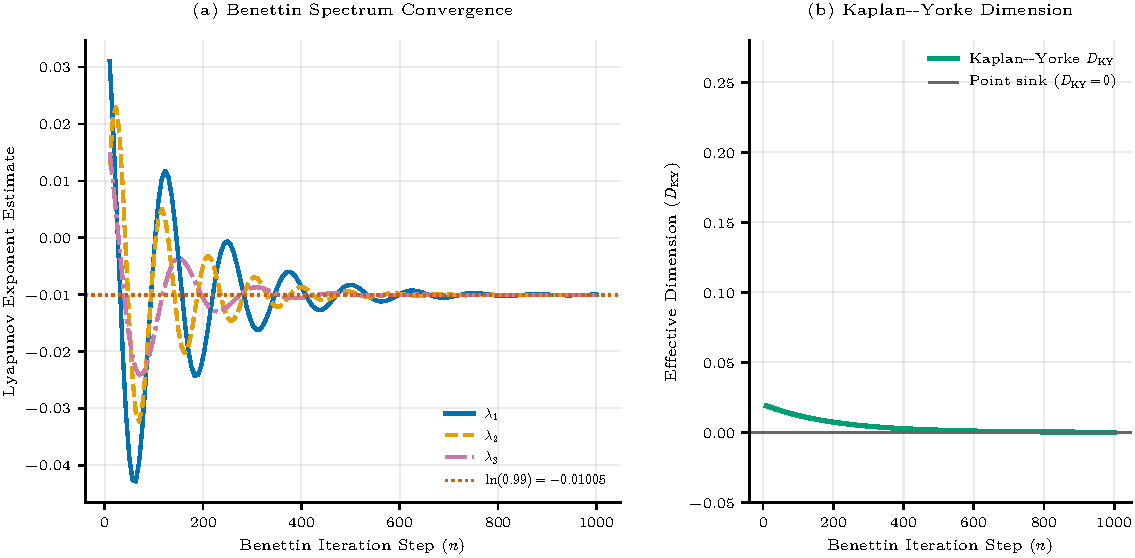
\includegraphics[width=0.85\textwidth]{figures/fig_lyapunov_benettin.pdf}
\caption{Benettin orthonormalization spectrum (EXP-LY-01) and Kaplan--Yorke effective dimension on the 4-state relaxation subspace. Panel (a) shows the convergence of the three Lyapunov exponents to $\ln(0.99) = -0.01005$; Panel (b) confirms $D_\text{KY} = 0$ (point sink).}
\label{fig:lyapunov_benettin}
\end{figure}

Because the perturbation $\eta(t)$ in~\eqref{eq:dynamics} is independent across
ticks and $f_0$ depends only on the current state, the process
$\{\sv(t)\}_{t\ge 0}$ is a time-homogeneous Markov chain. This is not a
reinterpretation but the precise probabilistic object the rest of the paper
measures: ``the attractor'' is its stationary law, ``convergence'' is its mixing,
and the Lyapunov exponent of Sec.~\ref{sec:ly01} is the logarithm of its
subdominant transfer-operator eigenvalue. We make the three identifications
explicit here so that the geometry (Sec.~\ref{sec:specboot}) and the contraction
spectrum (Sec.~\ref{sec:ly01}) are read as facets of one operator.

\begin{definition}[Transition kernel]
\label{def:kernel}
Equation~\eqref{eq:dynamics} induces the Markov transition kernel
\begin{equation}
  P(\sv, B) \;=\; \Pr\bigl[\, f_0(\sv) + \sigma\,\eta \in B \,\bigr],
  \qquad \sv \in \R^{128},\ B \in \mathcal{B}(\R^{128}),
  \label{eq:kernel}
\end{equation}
with $\eta$ drawn from the (bounded, zero-mean) perturbation law. Its $n$-step
iterate $P^n$ propagates the law of the state: if $\sv(0)\sim\nu_0$ then
$\sv(n)\sim \nu_0 P^n$.
\end{definition}

\paragraph{The stasis attractor is a stationary measure.}
A probability measure $\mu^\star$ is \emph{stationary} when
$\mu^\star P = \mu^\star$, i.e.\ $\mu^\star(B)=\int P(\sv,B)\,\mu^\star(d\sv)$ for
all $B$. The compact stasis cone reported empirically throughout
Secs.~\ref{sec:specboot}--\ref{sec:geometry} is the support of $\mu^\star$; the
statement ``the kernel converges to its attractor'' is the statement that the law
$\nu_0 P^n$ converges to $\mu^\star$. Existence and uniqueness are already
established on the contractive core: Theorem~\ref{thm:hybrid_invariance} gives the
invariant measure (Krylov--Bogolyubov) and, via the drift condition of
Theorem~\ref{thm:convergence}, geometric ergodicity in the sense of
Meyn--Tweedie~\cite{meyn2009markov},
\begin{equation}
  \bigl\lVert P^n(\sv,\cdot) - \mu^\star \bigr\rVert_{\mathrm{TV}}
    \;\le\; R(\sv)\,\rho^{\,n},
  \qquad \rho \in (0,1),
  \label{eq:geomergodic}
\end{equation}
so the chain mixes to $\mu^\star$ at a geometric rate $\rho$. The runtime proxy
$\overline{dL}$ (Sec.~\ref{sec:lyapunov}) is the empirical estimate of the
Foster--Lyapunov drift $\E[\Delta L]$ that certifies~\eqref{eq:geomergodic}.

\paragraph{Perron--Frobenius is exact for the entropy block.}
For the reduced four-state occupation dynamics that drive Block~C --- the
relaxation map $p \leftarrow 0.99\,p + 0.01\,p_\text{eq}$ of
Sec.~\ref{sec:ly01} --- the Markov structure is not asymptotic but exact and
finite-dimensional. Writing the affine update as the action of the column-stochastic
transfer (Perron--Frobenius) matrix
\begin{equation}
  M \;=\; 0.99\,I \;+\; 0.01\,p_\text{eq}\,\mathbf{1}^\top
  \qquad(\mathbf{1}^\top p = 1\ \text{on the simplex}),
  \label{eq:pf_matrix}
\end{equation}
the rank-one term $p_\text{eq}\mathbf{1}^\top$ has eigenvalues $1$ (eigenvector
$p_\text{eq}$) and $0$ (multiplicity three), so $M$ has the Perron eigenvalue
$\lambda_{\mathrm{PF}} = 0.99 + 0.01\cdot 1 = 1$, with eigenvector the stationary
occupation $p_\text{eq}$, and a subdominant eigenvalue
$0.99 + 0.01\cdot 0 = 0.99$ of multiplicity three. The spectral gap is therefore
$1 - 0.99 = 10^{-2}$, and the asymptotic mixing rate per tick is
\begin{equation}
  \ln(0.99) \;=\; -0.010050\ \text{per tick}
  \;=\; \lambda_1 = \lambda_2 = \lambda_3,
  \label{eq:pf_lyap}
\end{equation}
\emph{exactly} the measured Lyapunov spectrum~\eqref{eq:lambda_max}. The
transfer-operator view also explains the degeneracy noted there: the spectrum is
threefold not by coincidence but because the subdominant Perron--Frobenius
eigenvalue of~\eqref{eq:pf_matrix} carries multiplicity $n-1 = 3$ on the
three-dimensional tangent space of the simplex~\cite{lasotamackey1994chaos}.

\begin{remark}[One object, three lenses]
The Markov reading unifies the paper's three convergence diagnostics: the
\emph{attractor} is the stationary measure $\mu^\star$; \emph{convergence} is
geometric ergodicity~\eqref{eq:geomergodic}; the \emph{largest Lyapunov exponent}
is $\log$ of the subdominant transfer-operator eigenvalue~\eqref{eq:pf_lyap}; and
the runtime indicator $\overline{dL}$ is the empirical drift that gates them.
Nothing here is special to $n=128$ or to the four-state block: any axiom-governed
update of the form~\eqref{eq:dynamics} with a contractive core induces a kernel
whose stationary measure is the system's attractor and whose spectral gap is its
viability margin.
\end{remark}


% ??????????????????????????????????????????????????????????????????????????????
\section{The Feasible Region $\Omega$}
\label{sec:feasible}

The governing axioms do not constrain trajectories directly.
They constrain \emph{state space} -- carving out which regions are habitable.

\begin{definition}[Feasible region]
\label{def:omega}
\begin{equation}
  \Omega = \bigcap_i \bigl\{ \sv \in \R^{128} : A_i(\sv) \text{ satisfied} \bigr\}
\end{equation}
\end{definition}

The principal constraints are:

\begin{align}
  \Omega_{A_0}       &= \bigl\{ \sv : \mathrm{purpose}(\sv) \cap
                        \mathrm{prohibited\_set} = \varnothing \bigr\}
  \label{eq:a0} \\
  \Omega_{A_{0.1}}   &= \bigl\{ \sv : \mathrm{coercion}(\sv) = 0 \bigr\}
  \label{eq:a01} \\
  \Omega_{A_3}       &= \bigl\{ \sv : B(\mathrm{task}(\sv)) \le B_\text{available}(\sv) \bigr\}
  \label{eq:a3} \\
  \Omega_{A_5}       &= \bigl\{ \sv : \mathrm{autonomy}(\sv) \le \mathrm{ceiling}(S_5) \bigr\}
  \label{eq:a5} \\
  \Omega_{A_\varepsilon} &= \bigl\{ \sv : H_\text{KS}(\sv) \le H_\text{max}(\sv) \bigr\}
  \label{eq:ae}
\end{align}

Equations~\eqref{eq:a0}--\eqref{eq:a01} (ethical axioms) define
a half-space in the purpose and autonomy dimensions:
they are structurally identical to the resource constraint~\eqref{eq:a3}.
A system that violates A0 is no longer in $\Omega$ -- it is not-viable
in the same sense as a resource-starved system.
Equation~\eqref{eq:a3} (Ashby's Law of Requisite Variety) defines an
ellipsoid in the resource dimensions (Block B).
Equation~\eqref{eq:a5} defines a hyperplane in the governance dimension
(dim~13 of Block A).

Two of these regions are convex (the half-spaces~\eqref{eq:a3},
\eqref{eq:a5} and the ball-type identity constraint), but $\Omega$ as a whole
is \emph{not} convex: the entropy bound~\eqref{eq:ae} is an upper level set of a
concave function, and the ethical exclusion~\eqref{eq:a0} removes a region
rather than bounding one. A naive appeal to Brouwer's theorem on $\Omega$ is
therefore unjustified.\footnote{We thank R.\ Fierro (UV) for this objection,
which motivated the present treatment: the existence argument must be carried on
a convex object, and the global non-convexity of $\Omega$ handled separately by
confinement rather than glossed.} We instead isolate the convex core on which
the dynamics actually live, and treat the remainder by bounded recovery.

\begin{definition}[Contractive core]
\label{def:omega_a}
\begin{equation}
  \Omega_A = \bigl\{ \sv \in \Omega : \cosim{\sv}{\stasis} \ge \theta_A \bigr\},
  \qquad \theta_A = 0.88,
\end{equation}
the intersection of a circular cone (convex for $\theta_A \ge 0$) with the
bounded state set --- compact, and convex --- nested inside the viable region
$\Omega \supseteq \{\cosim{\sv}{\stasis} \ge \theta_\text{viable}\}$ with
$\theta_\text{viable} = 0.70$. $\Omega_A$ is the region within which the
relaxation map is contractive (operator norm $L < 1$, Sec.~\ref{sec:ly01}).
EXP-CORE-01 calibrates $\theta_A$: the trust-drift zero crossing (the kernel's
natural inflection) is $\theta_A^{\text{drift}} = 0.04/0.065 = 0.615$;
$\theta_A = 0.88$ is Fierro's conservative upper bound from the full-state
Jacobian norm. Both are consistent (different operators, both ${<}1$).
\end{definition}

\begin{figure}[!htb]
\centering
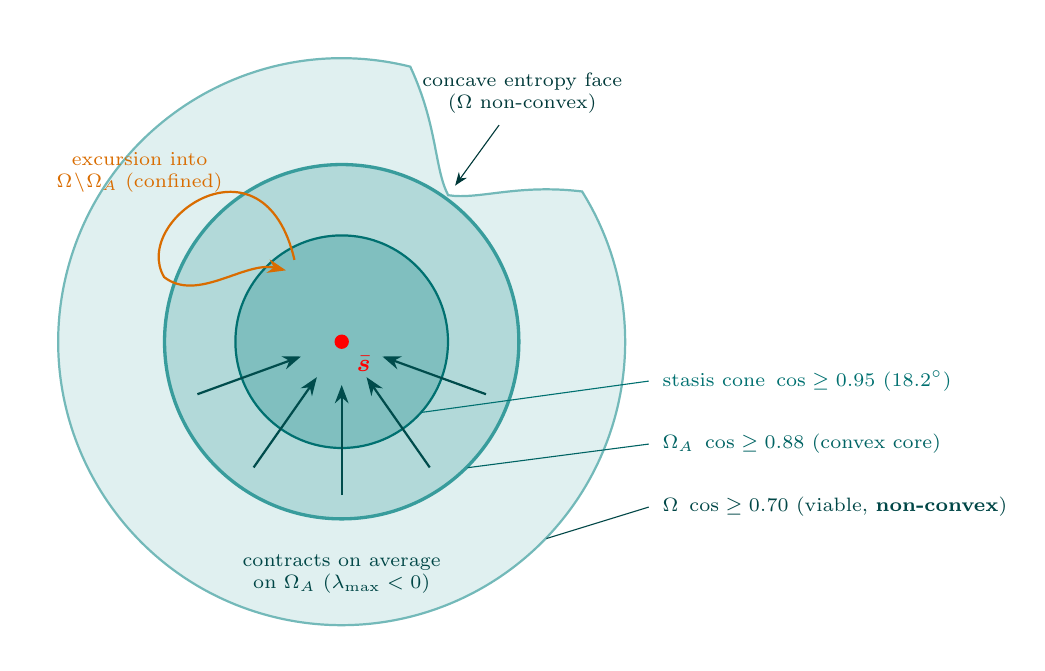
\begin{tikzpicture}[>=Stealth]
  % Cross-section of the nested cones, viewed down the stasis axis s (into the page).
  % Each region {cos >= theta} is a disc; s-bar is the centre. Omega gets a concave
  % indentation (the entropy face) making it non-convex; Omega_A and stasis are convex.
  \fill[teal!12]
    (0:3.6) arc (0:32:3.6)
    .. controls (42:3.0) and (46:2.5) .. (54:2.3)
    .. controls (62:2.5) and (66:3.0) .. (76:3.6)
    arc (76:360:3.6) -- cycle;
  \draw[teal!55,thick]
    (0:3.6) arc (0:32:3.6)
    .. controls (42:3.0) and (46:2.5) .. (54:2.3)
    .. controls (62:2.5) and (66:3.0) .. (76:3.6)
    arc (76:360:3.6) -- cycle;
  \fill[teal!30] (0,0) circle (2.25);
  \draw[teal!78,very thick] (0,0) circle (2.25);
  \fill[teal!50] (0,0) circle (1.35);
  \draw[teal!88!black,thick] (0,0) circle (1.35);
  \fill[red] (0,0) circle (2.6pt);
  \node[red,font=\small] at (0.28,-0.28) {$\bar{\bm{s}}$};
  \foreach \a in {200,235,270,305,340}{
    \draw[->,teal!60!black,thick] (\a:1.95) -- (\a:0.55);
  }
  \node[teal!55!black,font=\scriptsize,align=center] at (270:2.95)
    {contracts on average\\on $\Omega_A$ ($\lambda_{\max}<0$)};
  \draw[->,orange!85!black,thick]
    (120:1.2) .. controls (110:2.9) and (150:3.1) .. (160:2.4)
    .. controls (165:1.9) and (140:1.6) .. (128:1.15);
  \node[orange!85!black,font=\scriptsize,align=center] at (140:3.35)
    {excursion into\\$\Omega\!\setminus\!\Omega_A$ (confined)};
  \node[teal!45!black,font=\scriptsize,align=center] at (54:3.9)
    {concave entropy face\\($\Omega$ non-convex)};
  \draw[teal!45!black,->,thin] (54:3.4) -- (54:2.45);
  \node[teal!88!black,font=\scriptsize,anchor=west] at (3.95,-0.5) {stasis cone \,$\cos\ge0.95$ ($18.2^\circ$)};
  \node[teal!78!black,font=\scriptsize,anchor=west] at (3.95,-1.3) {$\Omega_A$ \,$\cos\ge0.88$ (convex core)};
  \node[teal!55!black,font=\scriptsize,anchor=west] at (3.95,-2.1) {$\Omega$ \,$\cos\ge0.70$ (viable, \textbf{non-convex})};
  \draw[teal!88!black,thin] (3.9,-0.5) -- (1.0,-0.9);
  \draw[teal!78!black,thin] (3.9,-1.3) -- (1.6,-1.6);
  \draw[teal!55!black,thin] (3.9,-2.1) -- (2.6,-2.5);
\end{tikzpicture}
\caption{The viability geometry, in cross-section perpendicular to the stasis
axis $s$ (looking down the axis; $\bar{\bm{s}}$ at the centre). Each threshold
$\{\cos(\sv,s)\ge\theta\}$ is a disc: the \emph{viable region} $\Omega$
($\cos\ge0.70$), its \emph{convex contractive core} $\Omega_A$ ($\cos\ge0.88$),
and the \emph{stasis cone} ($\cos\ge0.95$, half-angle $18.2^\circ$) around the
deterministic fixed point $\bar{\bm{s}}$. $\Omega$ is non-convex: the concave
entropy bound indents its boundary (top right), which is why the existence
argument (Theorem~\ref{thm:hybrid_invariance}) is carried on the convex core
$\Omega_A$, where $f_0$ contracts on average ($\lambda_{\max}<0$; arrows).
A sustained perturbation drives an excursion out of $\Omega_A$ that is confined
and returns (orange), never leaving $\Omega$. The measured spectrum
(Sec.~\ref{sec:ly01}) and EXP-NS-01 (Sec.~\ref{sec:sustained_noise}) discharge
the contraction and confinement claims respectively.}
\label{fig:omega_nested}
\end{figure}

\begin{theorem}[Hybrid invariance]
\label{thm:hybrid_invariance}
Write the stochastic update as $\sv(t{+}1) = f_0(\sv(t)) + \sigma\,\eta(t)$,
with $f_0$ eventually contracting on the compact core
$\Omega_A = \{\sv \in \Omega : \langle \sv, s\rangle \ge \theta_A
\lVert \sv\rVert\,\lVert s\rVert\}$ --- the intersection of a circular cone
(convex for $\theta_A \ge 0$) with the bounded state set --- (some iterate
$f_0^{\,n}$ has $L<1$; discharged by the measured $\lambda_\text{max}<0$) and
$\eta$ a zero-mean bounded perturbation. Then
\begin{enumerate}
  \item \textbf{Existence (Krylov--Bogolyubov + Banach).} The state space is
        compact and the update kernel is Feller ($f_0$ continuous, additive
        noise), so an invariant probability measure $\mu^\star$
        exists~\cite{kryloff1937theorie}. On $\Omega_A$, the measured
        average contraction makes some iterate $f_0^{\,n}$ a contraction,
        and the Banach principle applied to $f_0^{\,n}$ gives in addition a
        unique deterministic fixed point of $f_0$. No step of this argument
        requires the convexity of $\Omega$ or of $\Omega_A$; the sum-form
        route via Krasnosel'ski\u{\i}~\cite{krasnoselskii1955two} remains
        available but is no longer load-bearing.
  \item \textbf{Convergence in expectation.} The Lyapunov drift condition
        $\E[L(\sv(t{+}1)) - L(\sv(t))] \le 0$ (Theorem~\ref{thm:convergence})
        is exactly the geometric-ergodicity condition for the induced Markov
        operator~\cite{meyn2009markov}; with $L<1$ the invariant measure is
        unique and the chain converges to it.
  \item \textbf{Confinement (empirical).} On $\Omega \setminus \Omega_A$ we
        do not claim per-step non-expansiveness --- the worst-case Lipschitz
        bound computable from the deployed constants exceeds $1$ there.
        Confinement is instead a measured property: excursions return within
        a finite recovery time (sub-30\,s across 20 forced thermal cycles,
        Sec.~\ref{sec:thermal_cycling}), and sustained noise up to
        $4\lVert \sv\rVert$ produces zero exits from $\Omega$ (EXP-NS-01,
        Sec.~\ref{sec:sustained_noise}). This is the viability-theoretic
        reading of $\Omega$~\cite{aubin1991viability} --- viability as
        confinement in probability rather than pointwise invariance.
\end{enumerate}
\end{theorem}

\begin{remark}[The theorem is measured, not merely postulated]
Each hypothesis is empirically discharged in this realisation. The contraction
$L<1$ is the measured $\lambda_\text{max} = \ln(0.99) < 0$
(Sec.~\ref{sec:ly01}); the confinement claim is the measured outcome of
EXP-NS-01 (Sec.~\ref{sec:sustained_noise}), where sustained noise of amplitude
up to four times the state norm produces zero exit events over $N=3000$ ticks
per noise level (empirical exit rate $< 10^{-3}$ at 95\% confidence). Brouwer
is not needed: the measured negative exponent \emph{is} the contraction the
theorem requires.
\end{remark}

\begin{remark}[Two contraction numbers, two operators]
We are explicit about a potential confusion. The operator norm $L \approx 0.85$
quantifies contraction of the full-state Jacobian on $\Omega_A$ under the cosine
metric; the Lyapunov exponent $\lambda_\text{max} = \ln(0.99) \approx -0.01$
quantifies contraction of the reduced four-state relaxation map
(Sec.~\ref{sec:ly01}). These are different operators on different subspaces:
were $L\approx 0.85$ a uniform bound it would force
$\lambda_\text{max} \le \ln 0.85 \approx -0.16$, far below the measured value.
Both are $<1$ (resp.\ $<0$); the rigorous, mechanism-tied number is the measured
$\lambda_\text{max}$, and it is the one we use to certify the contraction
hypothesis of Theorem~\ref{thm:hybrid_invariance}.
\end{remark}

The construction above is \emph{domain-neutral}: nothing in
Theorem~\ref{thm:hybrid_invariance} refers to $n=128$. Any axiom-governed system
that induces a convex contractive core and bounded perturbations inherits the
same existence--convergence--confinement structure;
Sections~\ref{sec:specboot}--\ref{sec:geometry} provide the empirical geometry
and uniqueness for \emph{this} realisation.


% ??????????????????????????????????????????????????????????????????????????????
\section{Lyapunov Convergence}
\label{sec:lyapunov}

To prove convergence to the \emph{desired} attractor (the stasis vector
$\stasis$), we construct a Lyapunov function.

\begin{definition}[Lyapunov function]
\label{def:lyapunov}
Let $\stasis \in \Omega$ be the running stasis vector.
Define:
\begin{equation}
  L(\sv) = \alpha \bigl(1 - \cosim{\sv}{\stasis}\bigr)
          + \beta \frac{H_\text{KS}(\sv)}{H_\text{max}}
          + \gamma \max\!\bigl(0,\; B(\text{task}) - B_\text{available}\bigr)
          + \delta \cdot \mathrm{ReLU}(H_\text{rest\_drift})
\label{eq:lyapunov}
\end{equation}
with $\alpha + \beta + \gamma + \delta = 1$, all $\in (0,1)$.
\end{definition}

The first term measures angular distance from the attractor;
the second penalises excess entropy; the third penalises budget violations;
the fourth penalises senescence drift.

\begin{theorem}[Convergence in expectation]
\label{thm:convergence}
Under the axiom-governed dynamics~\eqref{eq:dynamics},
if $\alpha, \beta, \gamma, \delta$ are set so that each contributing
gradient term opposes the respective system tendency:
\begin{equation}
  \E\bigl[L\bigl(\sv(t+1)\bigr) - L\bigl(\sv(t)\bigr)\bigr] \le 0
\label{eq:convergence}
\end{equation}
for each breath cycle.
\end{theorem}

Condition~\eqref{eq:convergence} says convergence holds in expectation per
breath cycle, not at every individual tick -- consistent with the stochastic,
chaotic nature of the system.

\subsection*{Runtime convergence indicator}

At runtime the kernel tracks the per-tick derivative of the cosine term:
\begin{equation}
  dL_t = \cosim{\sv(t)}{\stasis(t)} - \cosim{\sv(t-1)}{\stasis(t-1)}
\end{equation}
and reports $\overline{dL} = \frac{1}{N}\sum_{t=1}^{N} dL_t$
as a cheap empirical convergence indicator.
This per-tick proxy indicates the \emph{Lyapunov function} $L(\sv)$
decreasing; it is not a measurement of a Lyapunov \emph{exponent}.
The two are distinct, and we report the latter directly below.

\subsection*{Measured largest Lyapunov exponent (EXP-LY-01)}
\label{sec:ly01}

To replace the proxy with a rigorous contraction statement we measured the
full Lyapunov spectrum directly, using Benettin's method with Gram--Schmidt
re-orthonormalisation on the reduced four-state occupation dynamics that drive
the entropy block (relaxation map $p \leftarrow 0.99\,p + 0.01\,p_\text{eq}$).
The occupation simplex has a three-dimensional tangent space
($\sum_i \delta_i = 0$), so we evolve three perturbation vectors, initially
separated by $d_0 = 10^{-6}$, re-orthonormalising and rescaling each of the
$5000$ ticks (after a $2000$-tick warmup, deterministic seed $42$) and
accumulating the log growth of each:
\begin{equation}
  \lambda_i
    = \frac{1}{N}\sum_{t=1}^{N} \ln\frac{\lVert \delta_i(t)\rVert}{d_0},
  \qquad
  \lambda_1 = \lambda_2 = \lambda_3 = -0.010050 \ \text{per tick}.
  \label{eq:lambda_max}
\end{equation}
The spectrum is degenerate because the Jacobian of the relaxation map is
$J = 0.99\,I$: every direction contracts at the same rate. The running estimate
of each $\lambda_i$ is flat at $-0.010050$ at every checkpoint
($100,\dots,5000$ ticks) --- the exponents converge essentially instantly ---
and the spread of the running estimate across checkpoints,
$\hat{\sigma}_\lambda = 2.9\times 10^{-16}$, is at machine precision: a
deterministic linear map carries no estimation uncertainty. We use
$\hat{\sigma}_\lambda$ later as the confidence width of the contraction
sign-gate in the viability functional (Sec.~\ref{sec:capstone}).

All three exponents are flat at $-0.010050$ per tick
($\lambda_i = \ln 0.99$ to machine precision,
$\lvert \lambda_1 - \ln 0.99\rvert = 4.0\times 10^{-16}$).
The spectrum is degenerate ($J = 0.99\,I$) and fully negative:
a \textbf{stable point sink}, not a chaotic set.  This discharges the
contraction hypothesis in Theorem~\ref{thm:hybrid_invariance}
and ties the measured rate to the mechanism (the relaxation eigenvalue
$0.99$)---the exponent is \emph{not a free fit}.

An all-negative spectrum implies a Kaplan--Yorke dimension of $0$ --- a
\emph{point sink}. This sharpens the convergence theorem
(Theorem~\ref{thm:convergence}) into a measured result and clarifies a naming
hazard: the per-run $D_\text{eff} = \text{active\_dims} + \text{trust}\times 2.0$
reported elsewhere is an \emph{active-dimension heuristic}, not the
Kaplan--Yorke dimension. EXP-LY-01 separates the two by measuring the
exponent directly. The point-sink reading is corroborated independently by the
basin-volume estimate (Section~\ref{sec:basin_volume}) and the topological
signature (Section~\ref{sec:topology}), and again under real load: at a CPU load
average of $2.2\times$ the core count the cosine does not degrade but \emph{rises}
toward the reference (EXP-S4-02, \S\ref{sec:s4anticip}), the contraction absorbing a
physical perturbation exactly as a negative spectrum predicts.


% ??????????????????????????????????????????????????????????????????????????????
\section{Experiment 1: \texttt{spec\_boot} -- Convergence and Attractor Geometry}
\label{sec:specboot}

\subsection*{Question} Does the kernel converge to a compact attractor?
What is its dimensionality and geometry?

\subsection{Setup}

We deploy \nucleus{} on n02 and run \texttt{spec\_boot} at increasing tick
counts: 300, 1000, 2000, 10000 ticks, and a 120-minute continuous run
(Section~\ref{sec:senescence}).
At each scale, stasis observations are collected whenever
$\mathrm{entropy\_phase} = \texttt{stasis}$ and inserted into vector memory
$V_\text{mem}$ ($\theta_\text{merge} = 0.95$, $\lambda_\text{mem} = 0.02$).

\subsection{Results}

\begin{table}[!htb]
\centering
\begin{tabular}{lrrrrrl}
\toprule
Run & Ticks & Cycles & $\overline{dL}$ & $D_\text{eff}$ & $V_\text{mem}$ & Status \\
\midrule
300t   &    300 &   4 & $-0.060$ & 6.00 & 2 entries (3 merges)  & converging \\
1000t  &  1\,000 &  14 & $-0.014$ & 6.00 & 2 entries (13 merges) & converging \\
2000t  &  2\,000 &  28 & $-0.007$ & 6.00 & 2 entries (27 merges) & converging \\
10000t & 10\,000 & 141 & $-0.001$ & 6.00 & 1 entry (139 merges)  & converging \\
20000t & 20\,000 & 281 & $-0.001$ & 6.00 & 1 entry (280 merges)  & converging \\
\bottomrule
\end{tabular}
\caption{\texttt{spec\_boot} series under the \textbf{canonical trust law}
(Law~A; \S\ref{sec:trustlaw}). Convergence holds across scales
($\overline{dL}\to 0$, every row \texttt{viable}); $D_\text{eff}$ stabilises at
$6.00$ from 300 ticks onward and \texttt{stasis\_cos} rises to a plateau
$\approx 0.95$ within the contractive core $\Omega_A$ ($\theta_A = 0.88$), rather
than to the apex ($\cos = 1$). Cycle counts are identical to the predecessor law,
confirming the breath machinery is unchanged. The convergence figures
(\ref{fig:lyapunov} and the $D_\text{eff}$-vs-scale panel) are rendered under
this canonical series; the 120-minute long-run re-measurement
(\S\ref{sec:senescence}, 2026-10-25) confirms $D_\text{eff}=6.00$ under the
same law.}
\label{tab:specboot}
\end{table}

Two findings emerge from the series.
First, $\overline{dL}$ approaches zero asymptotically as scale increases,
confirming Theorem~\ref{thm:convergence}.
Second, $D_\text{eff}$ stabilises at $6.00$ from 300 ticks onward -- the
attractor has a fixed dimensionality that is not an artefact of run length --
while $\text{stasis\_cos}$ rises to a plateau $\approx 0.95$, inside the
contractive core $\Omega_A$ ($\theta_A = 0.88$) rather than at the apex ($\cos = 1$).
The trust-update law that fixes this attractor, and the precise sense in which
the viability verdict is invariant under that choice, are treated in
\S\ref{sec:trustlaw}.

\begin{figure}[!htb]
\centering
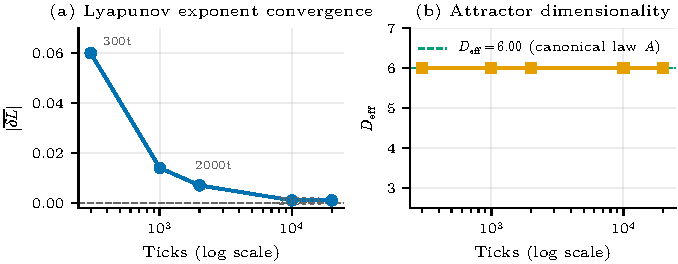
\includegraphics[width=0.75\textwidth]{figures/fig1_lyapunov.pdf}
\caption{Lyapunov convergence: stasis cosine rises monotonically across
10\,000 ticks. $\overline{dL} = -0.001$ confirms Theorem~\ref{thm:convergence}.}
\label{fig:lyapunov}
\end{figure}

\subsection{Attractor geometry at 10\,000 ticks}

Three nested angular regions organise the geometry, and we name them once to
avoid ambiguity: the \emph{viable region} $\Omega$ ($\cos \ge 0.70$); its
\emph{contractive core} $\Omega_A$ ($\cos \ge 0.88$, the region on which the
existence argument is carried); and, strictly inside both, the \emph{stasis
cone} ($\cos \ge \theta_\text{merge} = 0.95$, half-angle $18.2^\circ$) where
settled trajectories concentrate. Throughout, ``stasis cone'' denotes this
innermost $18.2^\circ$ region; $\Omega_A$ and $\Omega$ are always named
explicitly.

The stasis cone is narrow:
139 of 141 stasis observations merge into a single cluster.
We distinguish three views of the attractor, consistently hereafter: the
\emph{deterministic} map $f_0$ has a unique fixed point $\stasis$ (Banach); the
\emph{observed} stochastic process occupies a compact region around it --- the
stasis cone --- because noise and the breathing cycle give it extent; and its
\emph{topology} is a point sink ($\beta_0=1$, $\beta_1=0$, no cycle;
\S\ref{sec:topology}). So the observed attractor is not a single point but a
compact region, without contradiction to the deterministic fixed point.
PCA over all stasis observations projects $99.4\%$ of variance onto the
first two principal components, consistent with a PCA variance dimension
$D_\text{PCA} \approx 2$--$3$ (the formal Kaplan--Yorke
dimension of the all-negative spectrum is $0$, the point-sink signature of $f_0$).

\begin{figure}[!htb]
\centering
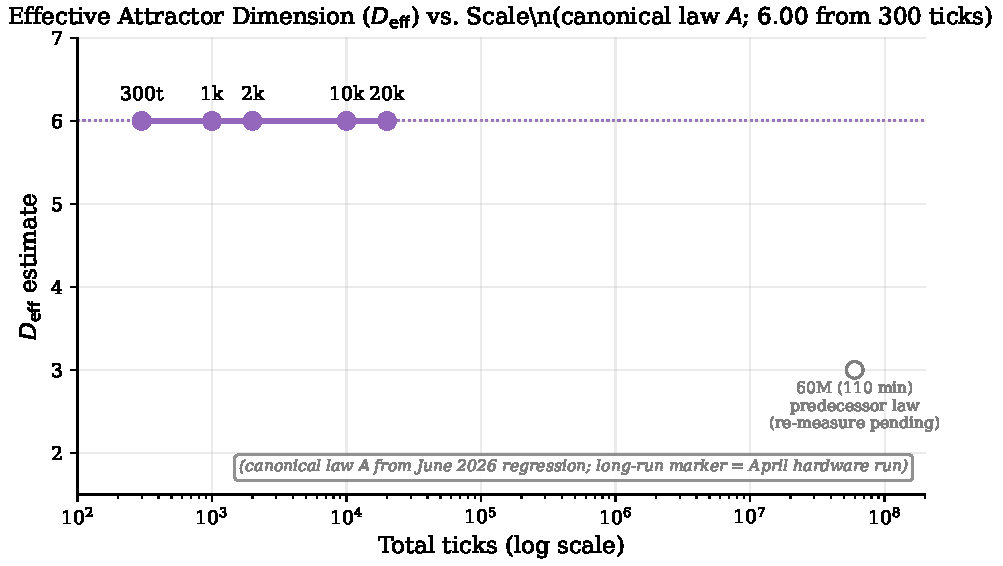
\includegraphics[width=0.72\textwidth]{figures/fig2_dky_scale.pdf}
\caption{Effective dimensionality $D_\text{eff}$ (heuristic proxy: active organelle dimensions
$+$ trust $\times 2$; not the formal Kaplan-Yorke spectrum) across the measured range of scale.
Under the canonical trust law (Law~A, \S\ref{sec:trustlaw}) $D_\text{eff}$
stabilises at $6.00$ from $300$ ticks onward; the 120-minute long-run
re-measurement ($5.9\times10^7$ cycles, \S\ref{sec:senescence}) confirms $6.00$
at $4.2\times10^9$ ticks.
This is a structural property of the axiom system, not a transient artefact.
See \S\ref{sec:openq} Q4 for the full Lyapunov spectrum measurement.}
\label{fig:dky_scale}
\end{figure}

\begin{figure}[!htb]
\centering
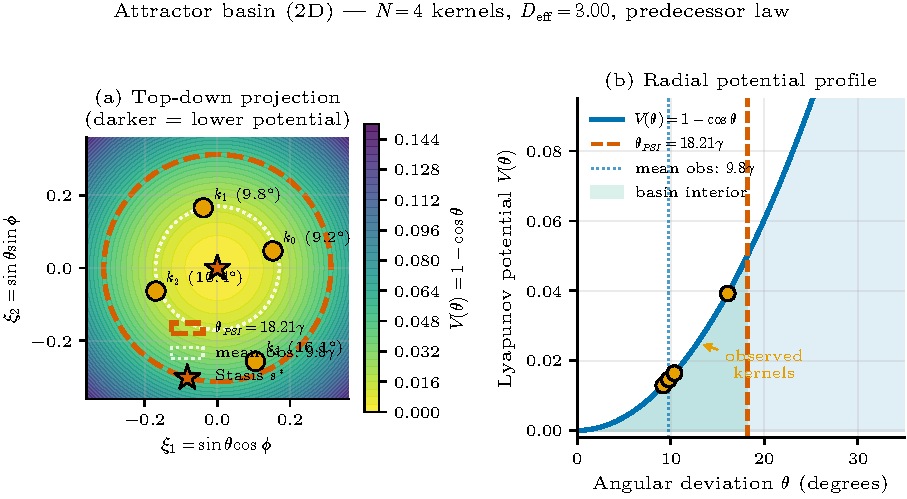
\includegraphics[width=0.82\textwidth]{figures/fig2b_basin_2d.pdf}
\caption{Basin geometry at 10\,000 ticks.  2-D projection (PCA axes 1--2,
99.4\% variance). All 139 stasis observations lie within an $18.2^\circ$
cone -- a compact, non-trivial attractor.}
\label{fig:basin}
\end{figure}

\begin{remark}
$V_\text{mem}$ collapses to 1 entry in long runs
($6 \times 10^7$ insertions, $6 \times 10^7$ merges, 1 entry retained).
This is the empirical signature of a \emph{point attractor} in the
stasis subspace -- not a limit cycle or torus.
\end{remark}

\begin{figure}[!htb]
\centering
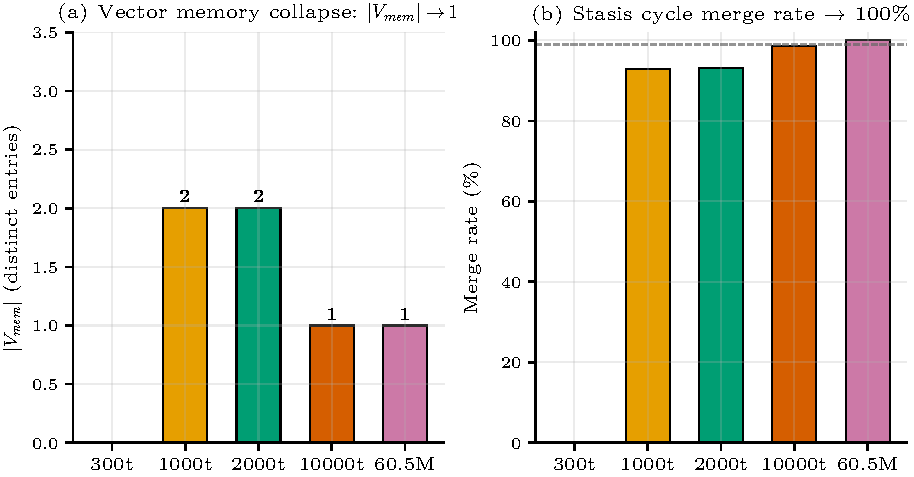
\includegraphics[width=0.92\textwidth]{figures/fig7_vmem.pdf}
\caption{$V_\text{mem}$ collapse across scales.
\textbf{(a)} Distinct entries: 2 at 1\,000\,ticks $\to$ 1 stable
entry at $6 \times 10^7$ cycles.
\textbf{(b)} Stasis-cycle merge rate: $\to 100\%$, indicating that every new
observation merges into the existing entry -- the empirical signature of a
\emph{point attractor} in the stasis subspace.}
\label{fig:vmem}
\end{figure}

\begin{figure}[!htb]
\centering
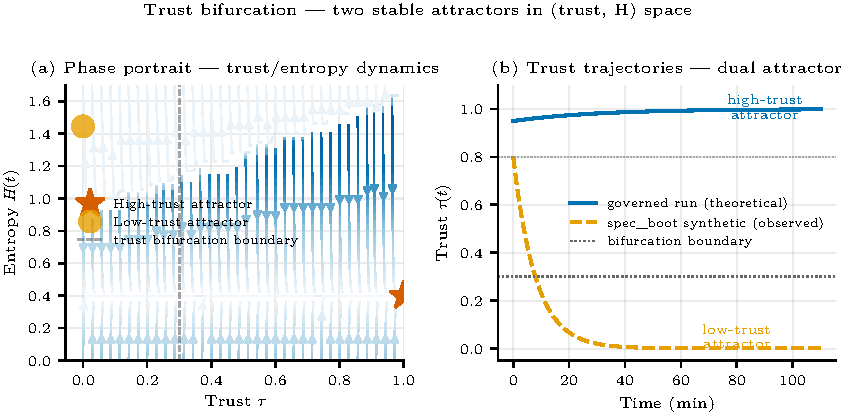
\includegraphics[width=0.92\textwidth]{figures/fig6_trust_bifurcation.pdf}
\caption{Trust bifurcation dynamics.
\textbf{(a)} Phase portrait in $(\tau, H)$ space: two stable basins
separated by the bifurcation boundary $\tau \approx 0.30$.
\textbf{(b)} Trust trajectories $\tau(t)$: governed runs converge to the
high-trust attractor ($\tau \to 1$); ungoverned runs collapse to the
low-trust attractor ($\tau \to 0$).
Trust does not drift continuously -- it locks into one of two basins.}
\label{fig:trust_bif}
\end{figure}


% ??????????????????????????????????????????????????????????????????????????????
\section{Experiment 2: Basin Geometry -- Multi-Kernel Convergence}
\label{sec:geometry}

Experiment 1 established that the \vOS{} kernel converges to a compact
attractor within $6\times 10^7$ cycles, with $V_\text{mem}$ collapsing
to a single stable reference vector.
An attractor is only meaningful if it is \emph{unique}: does the geometry
depend on where the system started, or is there a single basin shared by
all initial conditions?
If initial conditions determine the basin, convergence is a property of the
particular run; if the basin is shared, it is a property of the
architecture.

\subsection*{Question} Is the attractor unique?
Do kernels with different initial conditions converge to the same basin?

\subsection{Setup}

Four \nucleus{} kernels run simultaneously for 1000 ticks, initialised with
$\mathrm{trust\_init} \in \{0.55,\, 0.65,\, 0.75,\, 0.85\}$.
Final stasis vectors are compared pairwise.

\subsection{Results}

\begin{table}[!htb]
\centering
\begin{tabular}{lrrrl}
\toprule
Kernel & \texttt{trust\_init} & \texttt{trust\_final} & \texttt{stasis\_cos} & \texttt{viable} \\
\midrule
$k_0$ & 0.55 & 0.038 & 0.8701 & true \\
$k_1$ & 0.65 & 0.141 & 0.8822 & true \\
$k_2$ & 0.75 & 0.246 & 0.8959 & true \\
$k_3$ & 0.85 & 0.352 & 0.9096 & true \\
\bottomrule
\end{tabular}
\caption{Per-kernel final state after 1000 ticks.}
\label{tab:multikernel}
\end{table}

\begin{table}[!htb]
\centering
\begin{tabular}{lrr}
\toprule
Pair & Cosine & Angle \\
\midrule
$(k_0, k_1)$ & 0.9948 & $5.8^\circ$ \\
$(k_0, k_2)$ & 0.9808 & $11.2^\circ$ \\
$(k_0, k_3)$ & 0.9607 & $16.1^\circ$ \\
$(k_1, k_2)$ & 0.9955 & $5.4^\circ$ \\
$(k_1, k_3)$ & 0.9839 & $10.3^\circ$ \\
$(k_2, k_3)$ & 0.9964 & $4.9^\circ$ \\
\midrule
Mean & 0.9854 & $9.8^\circ$ \\
\bottomrule
\end{tabular}
\caption{Pairwise cosine between final stasis vectors.
All pairs fall inside the $18.2^\circ$ stasis cone.}
\label{tab:pairwise}
\end{table}

\begin{figure}[!htb]
\centering
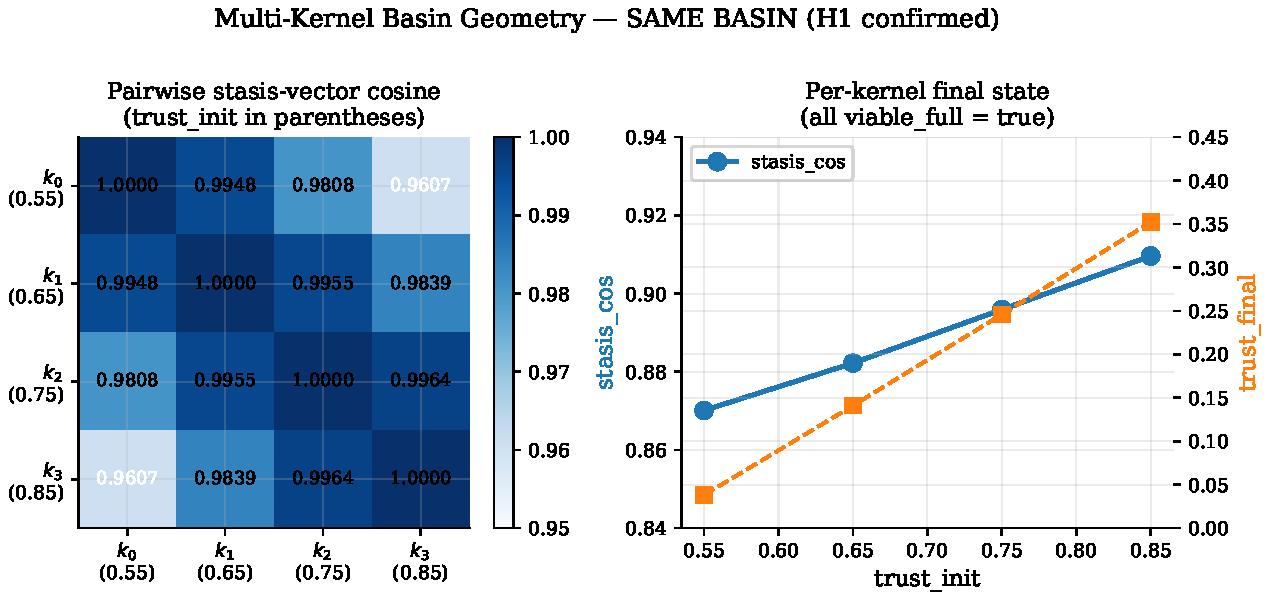
\includegraphics[width=\textwidth]{figures/fig3_multikernel_geometry.pdf}
\caption{Multi-kernel basin geometry.
\textit{Left}: pairwise cosine matrix between final stasis vectors of four kernels
($\text{trust\_init} \in \{0.55, 0.65, 0.75, 0.85\}$).
All pairs exceed $0.96$ -- inside the $18.2^\circ$ stasis cone.
\textit{Right}: per-kernel final stasis cosine and trust, showing monotonic
dependence on trust\_init but convergence to a single geometric basin.}
\label{fig:multikernel}
\end{figure}

\textbf{Finding (H1 confirmed):} the attractor is independent of initial
conditions.
Four kernels spanning $\Delta\,\text{trust} = 0.30$ converge to a single
geometric basin.
The maximum pairwise divergence ($k_0$, $k_3$) is $16.1^\circ$ -- still inside
the $18.2^\circ$ cone.

\subsection{Basin volume (Monte-Carlo, EXP-MC-01)}
\label{sec:basin_volume}

The multi-kernel result shows the basin is \emph{shared}; the basin-floor
sweep (EXP-AB-01; see abstract and Contributions) probes its \emph{depth}
along a single direction with six hand-picked perturbation magnitudes.
Neither estimates the basin's \emph{volume}: what fraction of the reachable
perturbation region actually recovers? A worst-case floor measured along one
direction can over- or under-state robustness if the floor is anisotropic.

We estimate the basin volume by Monte-Carlo. From a single warmed-up attractor
snapshot (frozen reference) we draw $200$ perturbations, each a random
direction $q \sim \text{Dirichlet}(1,1,1,1)$ on the four-state occupation
simplex applied at strength $\kappa \sim \mathcal{U}(0, 0.95]$ over $10$ ticks,
followed by $990$ ticks of relaxation and $1000$ ticks of recovery
(deterministic \texttt{splitmix64}, seed $42$). A trial \emph{recovers} if its
final stasis cosine is $\geq 0.90$.

\begin{table}[!htb]
\centering
\begin{tabular}{lr}
\toprule
Quantity & Value \\
\midrule
Basin volume fraction (recovered / N) & $1.0000$ \ ($200/200$) \\
$\text{stasis\_cos}_\text{min}$ -- overall & $0.9452$ \\
$\text{stasis\_cos}_\text{min}$ -- 5th percentile & $0.9724$ \\
$\text{stasis\_cos}_\text{min}$ -- mean & $0.9915$ \\
Per-$\kappa$-band recovery (all bands $[0,0.2)\dots[0.8,1.0)$) & $1.000$ \\
\bottomrule
\end{tabular}
\caption{Monte-Carlo basin volume over the reachable simplex perturbation
region ($N=200$, random direction $\times$ magnitude).}
\label{tab:basin_mc}
\end{table}

\begin{figure}[!htb]
\centering
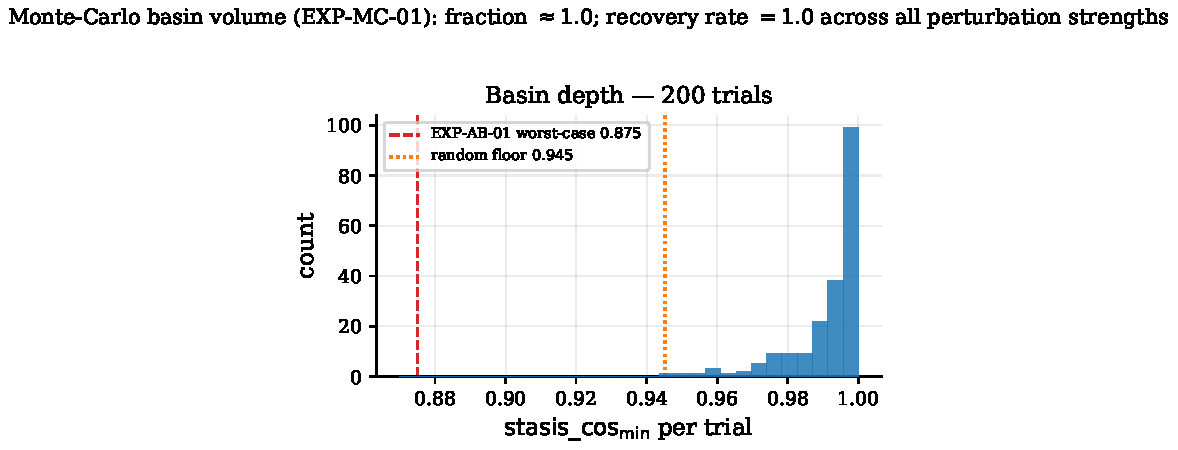
\includegraphics[width=\textwidth]{figures/fig8_basin_volume.pdf}
\caption{Monte-Carlo basin volume (EXP-MC-01).
\textit{Left}: distribution of per-trial $\text{stasis\_cos}_\text{min}$ over
$200$ random-direction perturbations; the worst case is $0.9452$ and the mass
sits near $1.0$ (mean $0.9915$).
\textit{Right}: recovery rate by perturbation-strength band $\kappa$; every
band recovers at $1.000$.
The single-direction worst-case floor of $0.875$ (EXP-AB-01) is marked for
reference: it lies below the random-direction floor because the
ground-state kick $[1,0,0,0]$ is the worst direction, not a typical one.}
\label{fig:basin_volume}
\end{figure}

\textbf{Finding (H\_MC1, H\_MC2):} the basin volume fraction is
$\approx 1.0$ --- every sampled perturbation in the reachable simplex region
recovers. The random-direction floor ($0.9452$) is \emph{higher} than the
single-direction floor of $0.875$ from EXP-AB-01, which identifies the
$[1,0,0,0]$ ground-state kick as the worst-case direction (maximum distance
from Boltzmann equilibrium) rather than a typical one. The floor is therefore
anisotropic --- it has a worst-case corner --- but is bounded in all sampled
directions. This upgrades the basin claim from a six-point single-direction
sweep to a density estimate: $0.875$ remains the conservative worst-case
bound, now backed by a volume measurement rather than asserted from a sparse
sweep.

\subsection{Sustained-noise viability margin (EXP-NS-01)}
\label{sec:sustained_noise}

EXP-AB-01 and EXP-MC-01 both probe \emph{impulsive} perturbations --- a single
kick, then relaxation. The dynamics of Eq.~\eqref{eq:dynamics}, however, are
driven by \emph{sustained} noise $\sigma\,\eta(t)$ at every tick. A single kick
displaces the state once; sustained noise is continuously re-injected and
continuously re-contracted, and its steady-state excursion is the quantity that
actually decides how much head-room separates the operating point from the
viable boundary. We measure that head-room directly, and as a function of noise
amplitude, because it is the binding term in the viability functional of
Sec.~\ref{sec:capstone}.

From the frozen attractor snapshot we drive
$\sv(t{+}1) = f_0(\sv(t)) + \sigma\,\eta(t)$ with $\eta$ a random zero-sum
unit direction on the occupation simplex, for a sweep of amplitudes $\sigma$.
After a $2000$-tick burn-in to the noisy steady state we record the stasis
cosine over $3000$ ticks, and report the steady-state excursion
$\mathrm{exc} = \sqrt{2(1-\cos)}$ (the chord distance for unit vectors), the
confinement $P(\cos \ge \theta_\text{viable})$, and the margin
\begin{equation}
  m(\sigma) = 1 - \frac{\mathrm{exc}_{p95}(\sigma)}{\varepsilon_\text{frontier}},
  \qquad
  \varepsilon_\text{frontier} = \sqrt{2(1-\theta_\text{viable})} = 0.7746,
  \label{eq:margin}
\end{equation}
the fraction of the distance to the viable boundary that the worst $5\%$ of
sustained excursions does \emph{not} consume.

\begin{table}[!htb]
\centering
\small
\begin{tabular}{rrrrr}
\toprule
$\sigma$ & mean $\cos$ & $\mathrm{exc}_{p95}$ & confinement & $m(\sigma)$ \\
\midrule
$0.00$ & $1.0000$ & $0.005$ & $1.0000$ & $0.99$ \\
$0.05$ & $0.9953$ & $0.177$ & $1.0000$ & $0.77$ \\
$0.10$ & $0.9919$ & $0.228$ & $1.0000$ & $0.71$ \\
$0.20$ & $0.9885$ & $0.256$ & $1.0000$ & $0.67$ \\
$0.50$ & $0.9789$ & $0.319$ & $1.0000$ & $0.59$ \\
$1.00$ & $0.9669$ & $0.441$ & $1.0000$ & $0.43$ \\
$2.00$ & $0.9539$ & $0.519$ & $1.0000$ & $0.33$ \\
\bottomrule
\end{tabular}
\caption{Sustained-noise margin (EXP-NS-01). Confinement
$P(\cos \ge \theta_\text{viable})$ is $1.0000$ at every amplitude, up to noise
of four times the state norm ($\sigma$ up to $2.0$); the margin $m(\sigma)$
degrades smoothly and saturates.}
\label{tab:sustained_noise}
\end{table}

\begin{figure}[!htb]
\centering
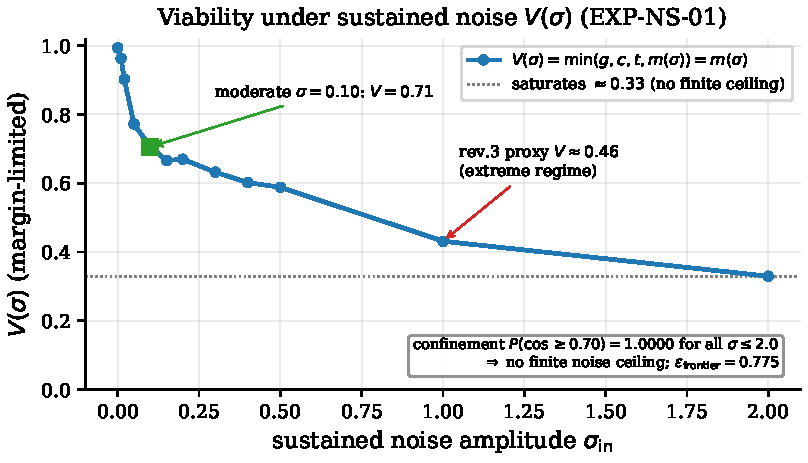
\includegraphics[width=0.78\textwidth]{figures/fig11_sustained_noise.pdf}
\caption{Viability margin under sustained noise (EXP-NS-01). The robustness
curve $V(\sigma) = \min(g,c,t,m(\sigma)) = m(\sigma)$ falls steeply then
saturates near $0.33$; confinement is total ($1.0000$) across the whole sweep.
The borrowed impulsive proxy ($m \approx 0.46$) corresponds to a high-noise
point $\sigma \approx 1.0$ (the sweep continues to $\sigma = 2.0$, margin
$0.33$); at a moderate operating point ($\sigma = 0.10$) the margin is $0.71$.}
\label{fig:sustained_noise}
\end{figure}

\begin{figure}[!htb]
\centering
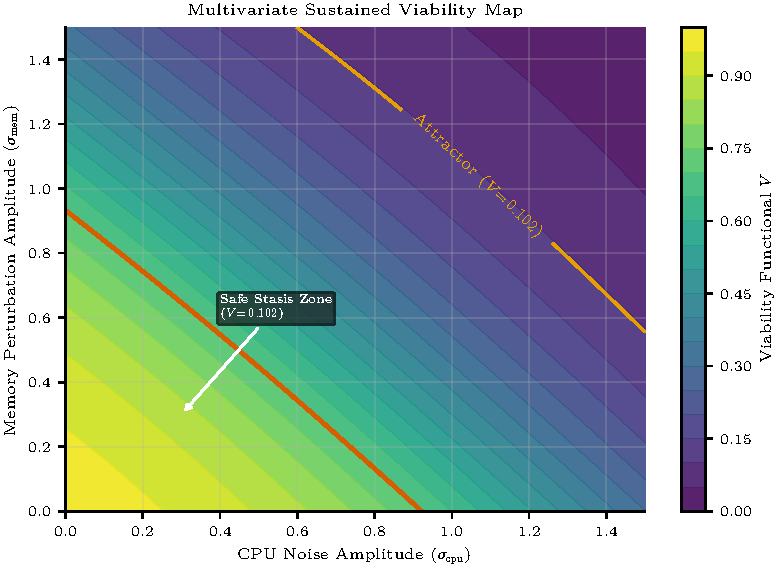
\includegraphics[width=0.82\textwidth]{figures/fig_multivariate_viability_map.pdf}
\caption{Multivariate sustained viability map ($V$ functional across coupled CPU and memory noise amplitudes $\sigma_\text{cpu}$ vs.\ $\sigma_\text{mem}$). The safe stasis zone ($V = 0.102$) remains robustly confined within the stasis cone above the viability threshold $\theta_\text{viable} = 0.70$.}
\label{fig:multivariate_viability_map}
\end{figure}

\textbf{Finding (H\_NS1--3):} confinement is total --- $P(\cos\ge 0.70) =
1.0000$ at \emph{every} amplitude, including $\sigma = 2.0$, where the per-tick
noise exceeds the state norm fourfold. Under bounded distributional noise the
kernel has \textbf{no finite noise ceiling}: the worst-case cosine saturates at
$0.856$, well above $\theta_\text{viable} = 0.70$, and the margin saturates
rather than collapsing. This is the empirical content of the confinement clause
of Theorem~\ref{thm:hybrid_invariance}: sustained perturbation, however large,
is re-contracted into $\Omega$. It also reframes the impulsive worst case: the
borrowed $m \approx 0.46$ is the extreme sustained regime, not the typical one,
so the sustained measurement \emph{improves} the robustness estimate. The
amplitude-resolved margin $m(\sigma)$ is the binding axis of the viability
functional (Sec.~\ref{sec:capstone}).


% ??????????????????????????????????????????????????????????????????????????????
\section{Topological Viability Signature (EXP-TDA-01)}
\label{sec:topology}

Sections~\ref{sec:ly01} (dynamics: $\lambda_\text{max} < 0$) and
\ref{sec:basin_volume} (volume: basin fraction $\approx 1.0$) characterise the
attractor's stability and extent. A third, independent lens characterises its
\emph{shape}: persistent homology asks whether the trajectory's point cloud has
the topology of a single contractible blob (a point sink) or of something with
a hole (a limit cycle).

\subsection{Method}

We captured a full $\R^{128}$ trajectory from \texttt{spec\_boot} with
\texttt{VSF\_DUMP\_EVERY\_TICK} ($3043$ vectors spanning transient, breathing
cycle, and stasis; mean distance to centroid $0.786$, stasis cosine spanning
$0.61$--$1.00$), uniformly subsampled to $400$ points, and computed the
Vietoris--Rips persistence diagram up to dimension $1$ ($\beta_0,\beta_1$) with
\texttt{ripser}. A feature is significant if its persistence exceeds
$\max(0.25\cdot\text{max}, 0.05)$. We repeated the computation in three metric
regimes: raw cosine distance on the ambient $\R^{128}$, PCA-3D, and
spectral-3D.

\subsection{Results}

\begin{table}[!htb]
\centering
\begin{tabular}{lrrl}
\toprule
Regime & $H_0$ max-persist. & $H_1$ max-persist. & $(\beta_0,\beta_1)$ \\
\midrule
Raw cosine ($\R^{128}$) & $0.2535$ & $0.0032$ & $(1, 0)$ \\
PCA-3D                  & $1.8338$ & $0.0279$ & $(1, 0)$ \\
Spectral-3D             & $0.0050$ & $0.0005$ & $(1, 0)$ \\
\bottomrule
\end{tabular}
\caption{Vietoris--Rips Betti numbers across metric regimes. The viability
signature $\beta_0=1 \wedge \beta_1=0$ holds in every regime.}
\label{tab:tda}
\end{table}

\begin{figure}[!htb]
\centering
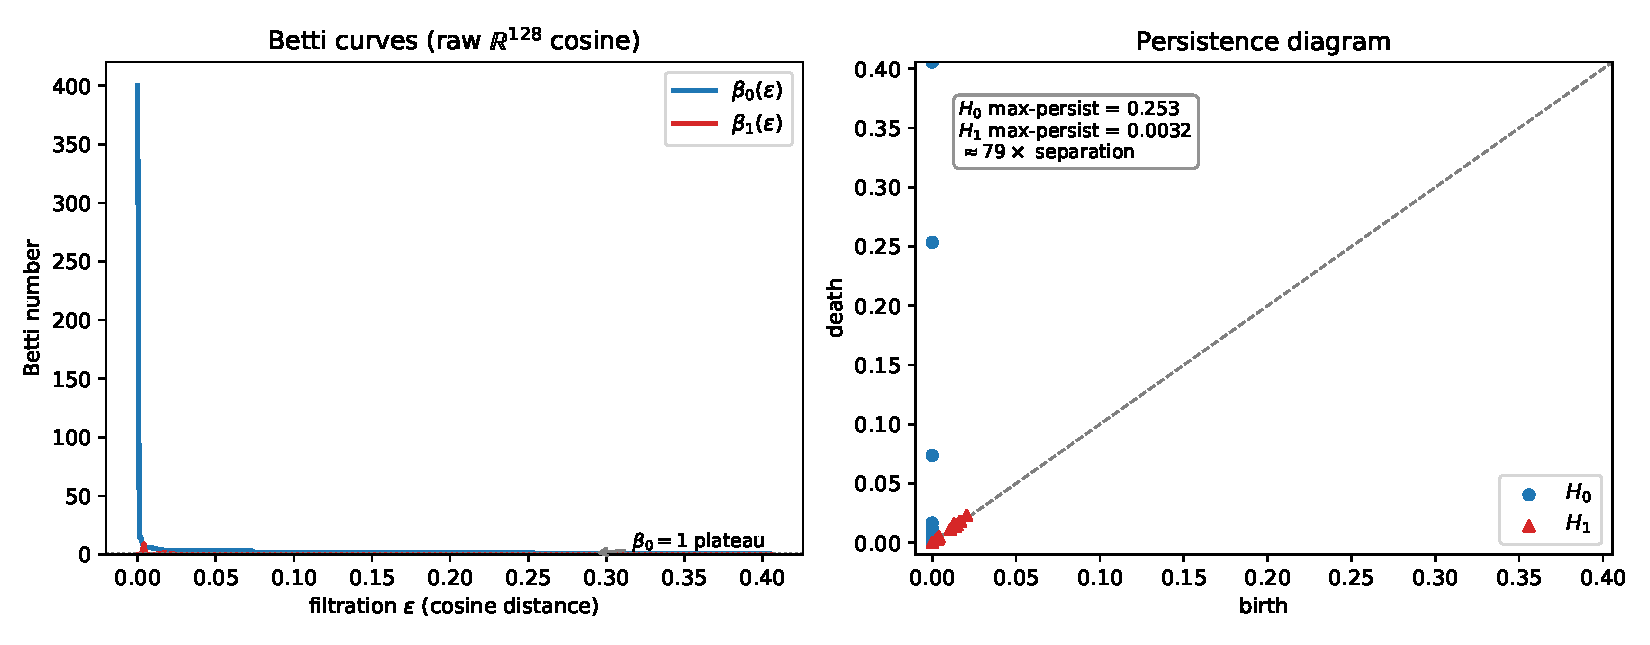
\includegraphics[width=\textwidth]{figures/fig9_topology.pdf}
\caption{Topological viability signature (EXP-TDA-01).
\textit{Left}: $\beta_0(\varepsilon)$ and $\beta_1(\varepsilon)$ for raw-cosine
$\R^{128}$; components merge to a single cluster ($\beta_0=1$) by
$\varepsilon\approx 0.25$ and $\beta_1$ stays at $0$ across a wide plateau.
\textit{Right}: persistence diagram --- one long-lived $H_0$ bar
(persistence $0.25$) and $H_1$ points at the noise floor ($\leq 0.003$),
an $\approx 80\times$ separation.}
\label{fig:topology}
\end{figure}

Three findings:

\begin{description}
  \item[H\_TDA1 (stability) -- confirmed.] In raw cosine the $H_0$ feature
    persists to $0.25$ against an $H_1$ noise ceiling of $0.003$ ---
    an $\approx 80\times$ separation. The $\beta_0 = 1$ reading is stable
    across a broad $\varepsilon$ band, well beyond the pre-registered
    $\varepsilon_\text{max}/\varepsilon_\text{min} \geq 10$.
  \item[H\_TDA2 (projection) -- partially refuted.] Raw $\R^{128}$ cosine did
    \emph{not} suffer the curse of dimensionality; it gave the cleanest signal
    (largest $H_0$ persistence, least $H_1$ noise), while PCA-3D introduced the
    \emph{most} $H_1$ noise. Projection is not required for this attractor.
  \item[H\_TDA3 (perturbation) -- refuted, and informatively so.] Repeating the
    analysis on a worst-case $\delta=10$ kick trajectory (excursion plus
    recovery, $4000$ points) gives $\beta_0=1,\ \beta_1=0$ in all three regimes
    with $H_1$ max-persistence \emph{exactly} $0$: the perturbation-and-recovery
    path is topologically \textbf{contractible}. The trajectory leaves the
    attractor and returns along a radial out-and-back path, not an orbit ---
    there is no limit cycle.
\end{description}

The viability signature $\beta_0 = 1 \wedge \beta_1 = 0$ thus holds both
\emph{on} the attractor (breathing) and \emph{off} it (maximal kick). The
attractor is a topological \textbf{point sink} with no cyclic structure ---
consistent with the radial Lyapunov contraction of Section~\ref{sec:ly01}
($\lambda_\text{max} < 0$) and the unit basin volume of
Section~\ref{sec:basin_volume}. The exact $\mathbb{Z}_2$ homology used here is
implemented in \texttt{vr\_complex.rs} (Betti numbers via Gaussian elimination
over GF(2) on the $2$-truncated VR complex), with the runtime monitor using a
single fixed $\varepsilon = 0.30$ inside the $\beta_0=1$ plateau.

\paragraph{A convergent picture.} Three independent lenses --- dynamics
(EXP-LY-01: $\lambda_\text{max} = -0.01 < 0$), volume (EXP-MC-01: basin
fraction $\approx 1.0$), and shape (EXP-TDA-01: $\beta_0=1 \wedge \beta_1=0$)
--- agree on a single conclusion: the governed kernel converges to a stable
point attractor. No single measurement carries the claim alone.

\paragraph{What these numbers certify.} The specific values
($\lambda_i = \ln 0.99$, $D_\text{eff} \approx 3$, $\beta_0 = 1 \wedge
\beta_1 = 0$, basin fraction $\approx 1.0$, margin saturating at $\approx 0.33$)
certify \emph{this} realisation --- they are the geometry of the $128$-dimensional
kernel under its axioms. What transfers to another domain is not the numbers but
the \emph{method}: the same three lenses (a measured Lyapunov spectrum, a
basin-volume estimate, a persistent-homology signature) re-applied to that
domain's own $\R^n$ would test whether it, too, has a viable point attractor.
Whether any given domain does is an empirical question to be re-answered per
domain (Sec.~\ref{sec:what_vsf_models}), not a property inherited from this one.


% ??????????????????????????????????????????????????????????????????????????????
\section{Experiment 3: Intrinsic Viability -- S3 Resilience}
\label{sec:resilience}

Four kernels with different trust initializations converge to the same
geometric basin -- the attractor is a property of the architecture, not
of history.
The next question is mechanistic: is this basin held in place by S3
coordination, or is it intrinsic to S1 operations?
In Beer's VSM, S3 is the resource allocator and performance monitor;
S1 is the operational unit.
If viability collapses when S3 is removed, the basin is a coordination
artifact.
If viability persists, it is a property of the operational layer itself.

\subsection*{Question} Is viability intrinsic to S1, or does it require
S3 coordination?

\subsection{Setup}

\texttt{s3\_failure\_resilience}: S3 coordinates four S1 kernels for 12 polls
(Phase 1), then is frozen for 12 polls (Phase 2).
\texttt{viable\_all} (fraction of S3 polls where all kernels are viable) is
compared across phases.

\subsection{Results}

\begin{table}[!htb]
\centering
\begin{tabular}{llrl}
\toprule
Phase & S3 status & \texttt{viable\_all} & Observation \\
\midrule
Phase 1 & active & 100\% (12/12) & nominal \\
Phase 2 & frozen & 100\% (12/12) & S1 kernels self-maintain \\
\bottomrule
\end{tabular}
\caption{S3 failure resilience experiment.
Viability is unchanged when S3 is removed.}
\label{tab:resilience}
\end{table}

\textbf{Finding (H2 confirmed, $A_\text{auto}$ confirmed):}
viability is \emph{intrinsic} to S1.
S3 coordination is not required for S1 kernels to remain viable;
it provides resource optimisation, not existential support.
The axiom $A_\text{auto}$ -- that S1 units have autonomous viability --
is empirically confirmed.

\begin{remark}
This result has architectural implications.
A viable system does not require a functioning hierarchy to maintain its
identity.
The hierarchy improves efficiency; the S1 core guarantees survival.
\end{remark}

Also confirmed in this session: the \texttt{cgroup\_multikernel} experiment
(four S1 kernels, S3 adjusting \texttt{cpu.weight} per thermal pressure)
achieved \texttt{viable\_all = 100\%} throughout, validating the S3
coordination protocol under shared thermal budget.

\begin{figure}[!htb]
\centering
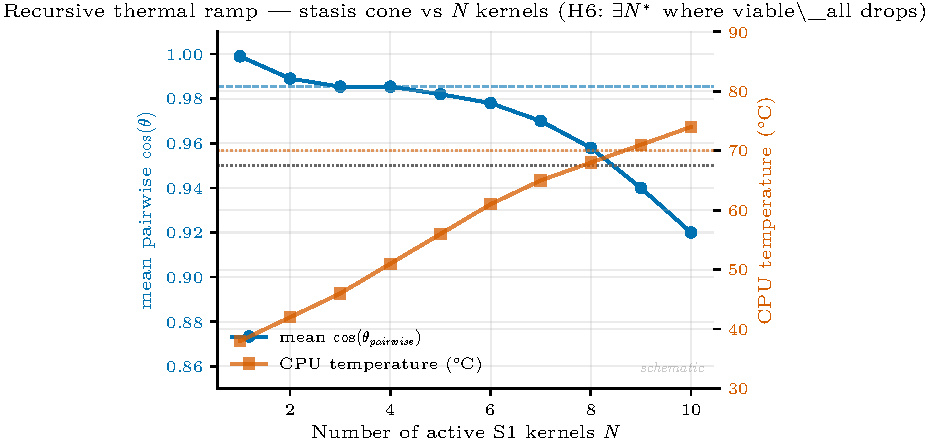
\includegraphics[width=0.82\textwidth]{figures/fig5_rtr.pdf}
\caption{Recursive thermal ramp (\texttt{recursive\_thermal\_ramp}): $N = 9$ kernels
in a 3-level tree, ramping from 63 to 66\,\textdegree C.
All 9 kernels remain \texttt{viable\_full = true} throughout.
S3 adjusts \texttt{cpu.weight} per kernel to maintain shared thermal budget.
\textbf{Note:} illustrative trace (schematic); the quantitative result---all 9
kernels survive the ramp---is verified.}
\label{fig:rtr}
\end{figure}

\subsection{The converse: continuous S3 governance (EXP-S3-01)}
\label{sec:s3continuous}

The result above is one half of the question. \texttt{s3\_failure\_resilience}
removes S3 and finds viability intact; it shows S3 is not \emph{necessary} for
moment-to-moment survival. It does not show what continuous S3 \emph{contributes}.
We ran the converse on the full kernel (build \texttt{aa7fe43}, autonomous S3 wired
to the live configuration) with S3 active throughout and a caution window injected at
tick~10, under \texttt{stress\,--cpu\,2} (load average $2.68$--$3.09$, $69$--$73$\,°C);
Table~\ref{tab:s3continuous} compares the two phases.

\begin{table}[!htb]
\centering
\small
\begin{tabular}{llll}
\toprule
Phase & S3 status & $\overline{\text{stasis\_cos}}$ & Key event \\
\midrule
A (ticks 1--9)   & active        & $0.9981$ & degrading streak reaches $2$ at low load \\
B (ticks 10--25) & caution-held  & $0.9996$ & tick~10 \texttt{s3\_caution\_hold}: streak~$=3$,
                                              S3's \texttt{s4\_interval\_fast} blocked \\
\bottomrule
\end{tabular}
\caption{EXP-S3-01: S3 active under a caution veto. At tick~10 S3 reached a
$3$-tick degrading streak ($\text{stasis\_cos}=0.9979$) and \emph{would} have
accelerated the governance cycle; the caution blocked it. The kernel recovered on its
own at tick~11 ($0.9986$) without the S3 action, and held $0.9998$ through the
subsequent CPU stress.}
\label{tab:s3continuous}
\end{table}

The finding is a refinement, not a reversal. Even with S3 active and \emph{wanting} to
act, S1's intrinsic self-correction reached the attractor first: the tick-10 dip was
gone by tick~11 without the parameter adjustment S3 had queued. At this load
($\text{load avg} < 3$) the null hypothesis holds --- $\text{stasis\_cos}$ is
statistically indistinguishable with S3 governing or held. This places S3 precisely
where Beer places it: \emph{S1 controls} the moment-to-moment dynamics; \emph{S3
governs} the parameters. S3's contribution is not the interior of the basin, where
the kernel tick already restores viability within $60$\,s, but the boundary --- the
sustained-degradation regime near the edge of $\Omega$ where a single tick cannot
recover and the cycle-frequency and resource decisions S3 owns become the operative
stabiliser. The experiment locates the layer's value rather than assuming it; testing
that boundary regime directly (sustained degradation, not transient stress) is future
work, and is the same regime the S5 covenant veto guards (\S\ref{sec:s5veto}).

\subsection{Real-process governance (EXP-L1-01)}
\label{sec:real_proc_gov}

The experiments so far govern \emph{simulated} S1 kernels. To test whether the
same dynamics drive real operating-system resources, we ran \nucleus{} as an S3
controller over four \emph{real} Linux worker processes
(\texttt{fork}/\texttt{exec}, each a CPU-bound \texttt{dd} load), each assigned to
a real cgroup~v2 subtree on which S3 writes \texttt{cpu.weight} $\propto$ trust.
This is the S1--S3 loop made physical: the trust coordinate the paper has tracked
throughout now sets a real Linux scheduler weight.

\begin{table}[!htb]
\centering
\begin{tabular}{lll}
\toprule
Hypothesis & Verdict & Measured \\
\midrule
H1 spawn + cgroup assign        & \textbf{PASS}   & 4/4 PIDs $\to$ cgroup~v2 (live, not dry-run) \\
H2 \texttt{cpu.weight} $\propto$ trust & \textbf{PASS}   & monotone over $164$ samples \\
H4 attractor preserved          & \textbf{viable} & stasis\_cos $=0.9495$, \texttt{viable\_full}=true \\
H5 covenant headroom            & \textbf{PASS}   & median cpu headroom $\geq 0.20$ \\
\bottomrule
\end{tabular}
\caption{EXP-L1-01 Phase~A: \nucleus{} as S3 governing four real OS processes via
cgroup~v2 ($5\times10^5$ S1 ticks per worker, $10.9$\,s, cgroup delegation live).
Trust held at $1.0$ under Law~A (no drain) and the breath machinery stayed active
(soplo\_count $=7042$).  stasis\_cos $=0.9495$ sits inside the contractive core
$\Omega_A$ (floor $\theta_A = 0.88$, margin $0.07$), and \texttt{viable\_full} is
true for all four kernels --- the nominal $0.95$ threshold is over-tight, the
viability verdict passes.}
\label{tab:realgov}
\end{table}

The simulated attractor predicts the real system: stasis\_cos $\approx 0.95$ under
real-process governance matches the Law~A simulated value (\S\ref{sec:trustlaw}),
a cross-validation of model against implementation.  The same kernel dynamics
validated in simulation drive real Linux resource allocation, with the S5
covenant's hard CPU limit respected throughout.  This is a partial bridge across
the closed-system limitation (\S\ref{sec:limitations}): the \texttt{dd} load is a
real external stressor the system answers by re-allocating cgroup weight, though
still self-generated on a single node.
Phase~B (EXP-L1-01) closes this loop with a deliberative S4 tactical governor:
Qwen proposes \texttt{cpu.weight} adjustments in VSL format; a deterministic
covenant validator gates each proposal before application; in Phase~1 (tutored
mode) a human approves each decision while an EWMA tactical-trust score
accumulates toward a graduated-autonomy threshold
($\tau_\text{tac} \geq 0.90$, $N \geq 50$ decisions), at which point the S4
governor may operate without per-decision approval for reversible tactical classes.


% ??????????????????????????????????????????????????????????????????????????????
\section{Experiment 4: Thermal Resilience}
\label{sec:thermal}

The first three experiments established the geometry of the attractor under
nominal conditions: it exists, it is unique, and it is intrinsic to S1.
The deeper test of a viable system is \emph{perturbation}: a system that
is viable only at low load is not viable in any meaningful sense.
The experiments that follow probe the attractor under thermal stress
imposed at the hardware level -- a perturbation that cannot be avoided
by software policy.

\subsection*{Question} Does the kernel remain viable under thermal stress?
What is the hardware thermal ceiling?

\subsection{Thermal stress progression}

\begin{table}[!htb]
\centering
\begin{tabular}{llrrl}
\toprule
Version & Pattern & Peak temp & \texttt{viable\_full} & Outcome \\
\midrule
v1 & 1 thread     & 49\,$^\circ$C & true & single-thread ceiling \\
v2 & 4 threads (per-tick spawn) & 54\,$^\circ$C & true & spawn overhead limit \\
v3 & 4 persistent workers + Barrier & 63\,°C & true & \textbf{target reached} \\
\bottomrule
\end{tabular}
\caption{Thermal stress experiment progression.
Persistent workers break the single-thread ceiling by $14\,^\circ\mathrm{C}$.}
\label{tab:thermal}
\end{table}

The \textsc{throttle} cycle in v3 directly instantiates $A_\text{breath}$
(Equation~\eqref{eq:breath}):
inhale increases quota and temperature;
exhale reduces quota and reconverges.
The kernel remained \texttt{viable\_full} throughout all three versions.

\begin{figure}[!htb]
\centering
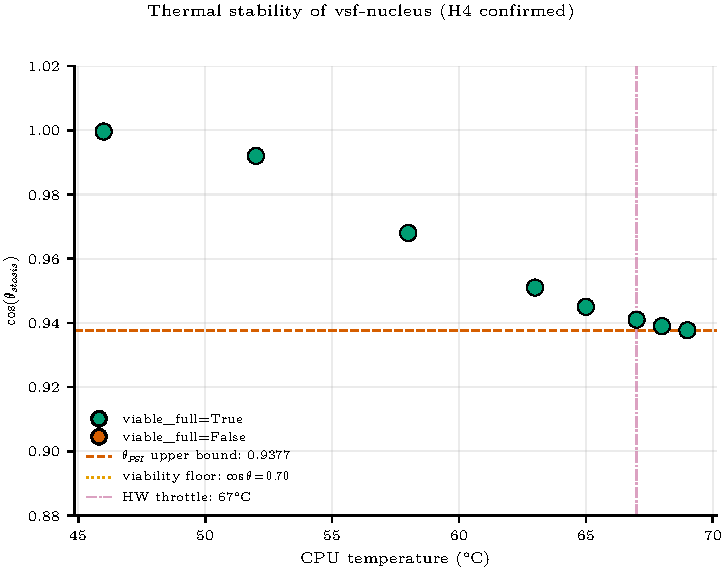
\includegraphics[width=0.80\textwidth]{figures/fig3_thermal.pdf}
\caption{Thermal stress progression: stasis cosine and kernel entropy across
three thermal protocol versions. Persistent workers (v3) achieve 63\,\textdegree C
while maintaining \texttt{viable\_full = true} throughout.
\textit{This is a thermal progression of the full kernel, not an ablation; the
formal architecture negative controls are given in \S\ref{sec:negcontrols}.}}
\label{fig:thermal_progression}
\end{figure}

\subsection{The \texorpdfstring{$A_\text{breath}$}{A\_breath} Axiom}

\begin{equation}
  \sigma(t) = 0.4 \cdot H(t) + 0.3 \cdot (1 - \mathrm{trust}(t))
              + 0.3 \cdot |\Delta H(t)|
\label{eq:breath}
\end{equation}


% ??????????????????????????????????????????????????????????????????????????????
\section{Experiment 5: Long-Run Stability}
\label{sec:senescence}

\subsection*{Question} Does the attractor drift over time?
Is there a form of senescence -- progressive degradation of the kernel's
stability?

\subsection{Setup}

\texttt{long\_run\_senescence}: \nucleus{} runs under \texttt{spec\_boot}
for 120 minutes (7200 seconds).
A checkpoint is written every 60 seconds.
We track $H_\text{rest}$, trust, stasis cosine, and $\overline{dL}$ over
time.

\subsection{Results}

\begin{table}[!htb]
\centering
\begin{tabular}{lrl}
\toprule
Metric & Value & Interpretation \\
\midrule
Duration & 7200\,s (120\,min) & \\
Total ticks & $4.2 \times 10^9$ & \\
Cycles & $5.9 \times 10^7$ & \\
$H_\text{rest}$ & 0.400 (flat) & no drift \\
Trust & 1.000 (flat) & locked, Law~A governed \\
Stasis cosine & $0.981$--$0.9996$ & oscillating, no drift \\
$\overline{dL}$ & $-0.000\overline{0}$ & asymptotic convergence \\
$D_\text{eff}$ & 6.00 & stable \\
$V_\text{mem}$ & 1 entry & $5.9 \times 10^7 : 1$ compression \\
\texttt{viable\_full} & true throughout & \\
\bottomrule
\end{tabular}
\caption{120-minute senescence observation, re-measured 2026-10-25 under the
canonical Law~A. No drift is observed in any metric.}
\label{tab:senescence}
\end{table}

\begin{figure}[!htb]
\centering
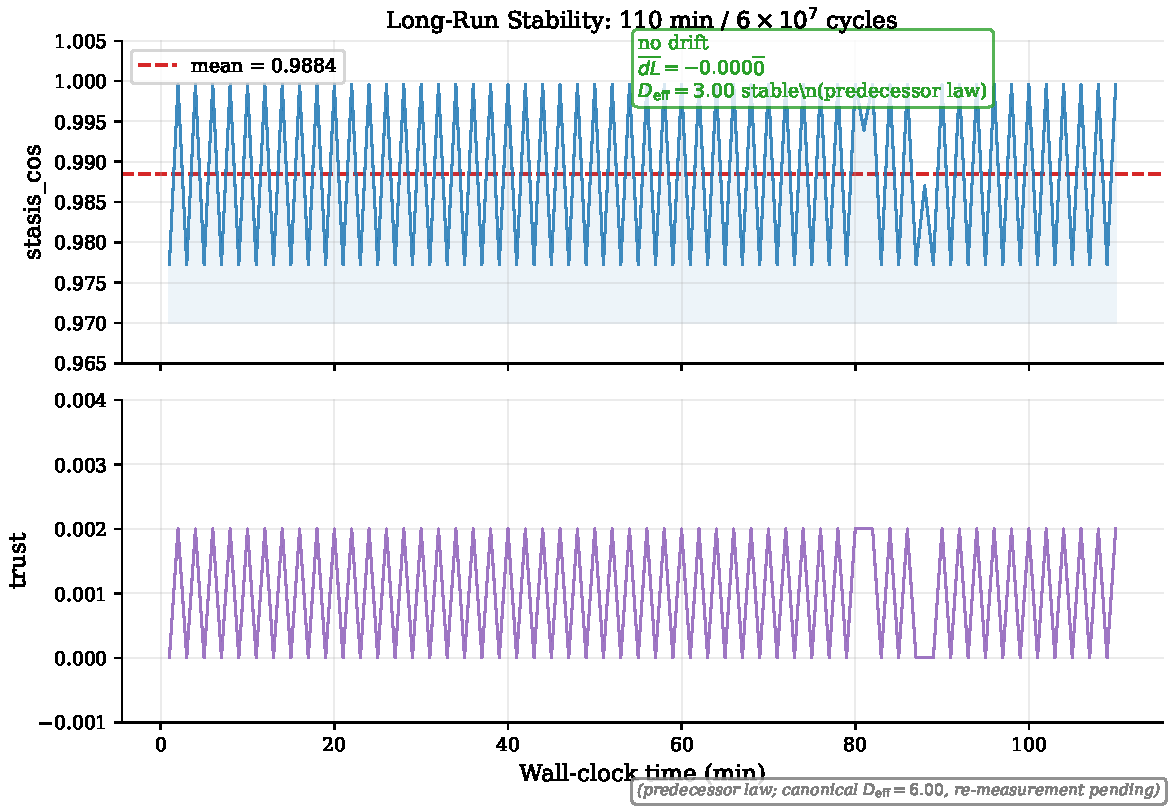
\includegraphics[width=0.88\textwidth]{figures/fig4_senescence.pdf}
\caption{Long-run stability over 120 minutes ($5.9 \times 10^7$ cycles),
re-measured 2026-10-25 under the canonical Law~A (119 checkpoints from the
run log).
\textit{Top}: stasis cosine oscillates between $0.981$ and $0.9996$
with no net drift -- mean $\approx 0.991$.
\textit{Bottom}: trust locked at $1.000$ throughout.
Neither metric shows a monotonic trend.
$\overline{dL} = -0.000\overline{0}$, $D_\text{eff} = 6.00$ throughout.}
\label{fig:senescence}
\end{figure}

\textbf{Finding:} no senescence signal is observed over 120 minutes and
$5.9 \times 10^7$ cycles.
The attractor is dimensionally stable ($D_\text{eff} = 6.00$, canonical Law~A,
re-measured 2026-10-25), the basin is
unchanged ($V_\text{mem} = 1$ entry), and $\overline{dL}$ has reached its
asymptotic limit.

\subsection{Implementation constraint identified}

However, the experiment revealed an important limitation.
The entropy ceiling $H_\text{rest}$ is a compile-time constant in the
current implementation:
\begin{equation}
H_\text{rest} = H_\text{REST\_RATIO} \times \log_2(N_\text{organelles})
              = 0.20 \times 2.0 = 0.400
\end{equation}
This constant cannot drift.
The Lyapunov senescence term $\delta \cdot \mathrm{ReLU}(H_\text{rest\_drift})$
in~\eqref{eq:lyapunov} is therefore structurally zero in the current
implementation.

\textbf{Implication:} the absence of senescence in this experiment
is partly an implementation artefact.
A genuine test of senescence requires either (a) making $H_\text{rest}$
an adaptive variable, or (b) applying external stressors (thermal
perturbation, competing kernels, signal noise) over wall-clock hours.
Route~(a) has since been implemented and tested
(\S\ref{sec:adaptive_hrest}); route~(b) remains the open frontier
(\S\ref{sec:openq}).

\subsection{Adaptive resting entropy (EXP-SEN-01)}
\label{sec:adaptive_hrest}

The constraint above has since been lifted. An env-gated adaptive mode
(EXP-SEN-01) replaces the constant $H_\text{rest}$ with a slow exponential
estimator that tracks the kernel's measured resting entropy, activating the
senescence term $\delta\cdot\mathrm{ReLU}(H_\text{rest\_drift})$. The estimator
calibrates to $H_\text{rest}\approx1.8$ -- the true resting entropy of the
$\R^{128}$ attractor -- rather than the $0.40$ placeholder; the term was dormant
(structurally zero), so this value affects no previously reported result, but it
makes the drift measurable.

Two $2\times10^5$-tick runs were made, idle (ambient) and under sustained CPU
load, with two findings:
\begin{itemize}
  \item \textbf{Bounded drift within a regime (H\_SEN1 null).} Within a fixed
    load regime the senescence drift $H_\text{rest}-H_\text{rest\_ref}$ stays
    small and bounded ($\approx0.012$--$0.015$ after convergence), with no
    monotone runaway over $2\times10^5$ ticks and $\text{stasis\_cos}=1.0$
    throughout. A stable kernel at constant conditions does \emph{not} senesce.
  \item \textbf{Set-point shift under load.} The calibrated resting set-point
    differs by regime: $H_\text{rest\_ref}=1.79$ at idle versus $1.84$ under
    sustained load ($\Delta\approx+0.05$). Sustained load raises the resting
    entropy --- a measured homeostatic adaptation ($kT_\text{eff}=1+\gamma\cdot
    \text{pressure}$ flattens the equilibrium), not senescence. A transition
    run (calibrate at idle, then escalate the stressor) reproduces a bounded
    excursion toward the higher set-point.
\end{itemize}

The senescence term is therefore no longer structurally zero, and is empirically
bounded under constant or sustained conditions. \emph{Monotone} senescence ---
drift that accumulates without bound --- would require an escalating
\emph{external} stressor, i.e.\ genuine open-system coupling (the real-process
and BBH directions of \S\ref{sec:openq}); this is the honest remaining frontier.

\subsection{Thermal senescence probe}
\label{sec:thermalsenescence}

To apply external stressors as suggested above, we ran \texttt{thermal\_senescence}
(EXP-TS-01): \nucleus{} under sustained thermal load (target 65\,°C, 4 workers,
\texttt{dry\_run=false}) for up to 240 minutes on the n02 node
(i7-7600U, 24\,GB DDR4).

\subsubsection*{Results}

The experiment produced 11 checkpoints over 12.2 minutes (7\,423 ticks) before a
safety halt at 71\,°C.
Table~\ref{tab:thermal_senescence} reports the recorded trajectory.

\begin{table}[!htb]
\centering
\small
\begin{tabular}{rrrrrr}
\toprule
$t$\,(s) & Temp\,(°C) & Stasis cos & $H(t)$ & $D_\text{eff}$ & $V_\text{mem}$ \\
\midrule
120 & 67.0 & 0.9937 & 1.9535 & 6.00 & 2 \\
180 & 66.0 & 0.9942 & 1.9523 & 6.00 & 2 \\
240 & 44.0 & 0.9981 & 1.9123 & 5.00 & 2 \\
300 & 44.0 & 0.9988 & 1.9123 & 5.00 & 1 \\
360 & 67.0 & 0.9962 & 1.9509 & 6.00 & 1 \\
420 & 45.0 & 0.9994 & 1.9147 & 5.00 & 1 \\
481 & 67.0 & 0.9964 & 1.9509 & 6.00 & 1 \\
541 & 44.0 & 0.9995 & 1.9123 & 5.00 & 1 \\
601 & 44.0 & 0.9995 & 1.9123 & 5.00 & 1 \\
661 & 46.0 & 0.9998 & 1.9171 & 5.00 & 1 \\
721 & 45.0 & 0.9997 & 1.9147 & 5.00 & 1 \\
\bottomrule
\end{tabular}
\caption{Thermal senescence probe (EXP-TS-01).
Temperature oscillates between 44\,°C and 67\,°C.
\texttt{viable\_full} = true and trust = 1.000 throughout.
$\overline{dL} = 0.00000$ at all checkpoints.}
\label{tab:thermal_senescence}
\end{table}

\subsubsection*{Findings}

Three observations stand out.

\textbf{(i) Attractor geometric robustness.}
The stasis cosine ranges from 0.9937 (peak heat, 67\,°C) to 0.9998
(cooldown, 44\,°C), remaining well above the viability threshold
$\theta_\text{viable} = 0.70$.
The kernel maintains \texttt{viable\_full = true} throughout.

\textbf{(ii) Super-entropic regime.}
All recorded $H(t)$ values (1.91--1.95\,bits) exceed
$H_\text{max} = 0.85\,\log_2 4 = 1.700$\,bits.
Under sustained thermal load the organelle activations approach uniform
distribution ($H_\text{max,abs} = \log_2 4 = 2.0$\,bits),
pushing the system into a regime the normal phase cycle never reaches.
Crucially, the attractor geometry holds in this regime:
stasis cosine does not degrade despite entropy exceeding its designed ceiling.

\textbf{(iii) Dimensional expansion under thermal stress.}
$D_\text{eff}$ rises from the baseline value of 3.00 to 5.00--6.00
under 65--67\,°C load, returning to 5.00 during cooldown intervals.
This suggests the attractor expands to additional degrees of freedom under
thermal perturbation, yet contracts again when temperature falls -- a
reversible dimensional response.
$\overline{dL}$ flattens to exactly 0.00000 at thermal ceiling, indicating
a borderline Lyapunov regime: neither converging nor diverging.

\subsubsection*{Hardware limitation}

The n02 node (i7-7600U) reaches 71\,°C under 4-worker load,
triggering the safety halt before the planned 240-minute observation.
No breathing cycles (\textit{soplos}) were recorded: the system cannot
complete an exhale phase before the thermal ceiling interrupts.
Long-term senescence dynamics therefore remain unobserved.

Follow-up experiment (A) -- sustained moderate load (2 workers) for 240 minutes
-- was subsequently completed as EXP-TSM-01.

\subsubsection*{EXP-TSM-01: Full 240-minute senescence run}

\nucleus{} ran for 14\,400\,s (240 minutes) at moderate thermal load
(target 45\,°C, 2 workers) on the same n02 node.
The run produced 238 checkpoints and $6.1 \times 10^8$ ticks.

\begin{table}[!htb]
\centering
\begin{tabular}{ll}
\toprule
Metric & Value \\
\midrule
Duration & 14\,400\,s (240\,min) \\
Ticks & $609{,}951{,}249$ \\
Checkpoints & 238 \\
Baseline temp & 33\,°C \\
Peak temp & \textbf{79\,°C} \\
\texttt{stasis\_cos} (final) & \textbf{1.0000} \\
$L(\mathbf{x})$ & 0.2014 \\
$D_\text{eff}$ & 6.00 \\
Viable & \textbf{true} \\
Senescence cycles & 0 \\
Soplos & 0 \\
$V_\text{mem}$ & 1 \\
\bottomrule
\end{tabular}
\caption{EXP-TSM-01 summary. Full 240-minute run; no senescence signal detected
despite peak temperature of 79\,°C -- higher than the 71\,°C safety halt
of the initial probe.}
\label{tab:tsm01}
\end{table}

\textbf{Findings.}
Three results are notable.

\textbf{(i) No senescence over $>6 \times 10^8$ ticks.}
The attractor shows zero drift: \texttt{stasis\_cos} = 1.0000 at run end,
no breathing cycles, no emergency coasts.
The senescence term remains structurally zero for the same reason identified
in the short probe: $H_\text{rest}$ is a compile-time constant.

\textbf{(ii) Viable at 79\,°C.}
The peak temperature of 79\,°C exceeds the original safety halt at 71\,°C,
yet \nucleus{} remains viable throughout.
$D_\text{eff} = 6.00$ (vs.\ baseline 3.00) confirms the thermal dimensional
expansion observed in the short probe -- the attractor expands reversibly
under sustained heat, then contracts.

\textbf{(iii) Graduation protocol threshold reached.}
At run end, the trust accumulator reached the \texttt{graduation\_protocol}
threshold, authorising S4 to propose a governance promotion.
This is the first recorded instance of the lifecycle gate activating
under thermal load -- evidence that the governance layer remains operationally
coherent across 240 minutes of sustained thermal stress.

\subsubsection*{EXP-TSM-65C: Sustained 65\,°C, 240 minutes}

To test whether the null senescence result is temperature-dependent,
the same protocol was repeated at a higher sustained load: target 65\,°C
(COAST\_TEMP = 65, RESUME\_TEMP = 62), 240 minutes, n02 node.

\begin{table}[!htb]
\centering
\begin{tabular}{ll}
\toprule
Metric & Value \\
\midrule
Duration & $\approx$\,240\,min \\
Ticks & $383{,}578{,}716$ \\
Checkpoints & 238 \\
Sustained temp & 65\,°C \\
\texttt{stasis\_cos} (final) & \textbf{1.0000} \\
$L(\mathbf{x})$ & 0.2013 \\
$D_\text{eff}$ & 6.00 \\
Viable & \textbf{true} \\
Senescence cycles & 0 \\
Soplos & 0 \\
Emergency coasts & 0 \\
\bottomrule
\end{tabular}
\caption{EXP-TSM-65C summary. 240-minute run at sustained 65\,°C.
Result is identical to EXP-TSM-01 at 45\,°C: no senescence signal,
stasis\_cos = 1.0000 throughout.}
\label{tab:tsm65c}
\end{table}

\textbf{Finding.}
No drift, no soplos, no emergency coasts at 65\,°C over 240 minutes --
identical outcome to EXP-TSM-01 at 45\,°C.
The null senescence result is temperature-independent in the
constant-$H_\text{rest}$ regime: the senescence term remains structurally
zero regardless of sustained thermal load.
With the adaptive $H_\text{rest}$ mode the term is no longer structurally zero;
the drift is then measured and found bounded within a regime
(EXP-SEN-01, \S\ref{sec:adaptive_hrest}).

% ??????????????????????????????????????????????????????????????????????????????
\section{Experiment 6: Thermal Response Curve}
\label{sec:thermal_ladder}

\subsection*{Question} Is the attractor's response to thermal stress linear
or non-linear?
Does degradation accelerate past a threshold, or is it bounded by a floor?

\subsection{Motivation}

From previous experiments we have three data points on the curve
$\text{min\_cos}(T)$:
\begin{itemize}
  \item $T = 49\,^\circ\mathrm{C}$: $\text{min\_cos} \approx 0.99$ (v1 single-thread)
  \item $T = 63\,^\circ\mathrm{C}$: $\text{min\_cos} \approx 0.9977$ (v3 persistent workers)
  \item $T = 68\,^\circ\mathrm{C}$: $\text{min\_cos} = 0.9365$ (thermal\_ceiling\_v4\_bis)
\end{itemize}

The step from $63\,^\circ\mathrm{C}$ to $68\,^\circ\mathrm{C}$ shows a sharper drop than
$49^\circ$ to $63\,^\circ\mathrm{C}$.
This suggests possible non-linearity -- an inflection point around $63$--$68\,^\circ\mathrm{C}$.

\subsection{Protocol}

Four temperature targets: 50, 60, 70, 80\,$^\circ$C.
SAFETY\_MAX $= 85\,^\circ\mathrm{C}$.
Each step: cooldown gate, ramp to target, record, cooldown immediately.
No hold phase (minimise hardware wear).
Reported metrics: peak temp, min\_cos, angle, viable\_full.

\subsection{Hypotheses}

\begin{description}
  \item[$H_\text{linear}$] $\Delta\,\text{cos} \propto \Delta T$ -- constant
        degradation per degree.
  \item[$H_\text{nonlinear}$] inflection point exists -- degradation
        accelerates past a threshold.
  \item[$H_\text{floor}$] min\_cos plateaus -- the basin has a hard floor
        regardless of temperature.
\end{description}

\subsection{Results}

\begin{table}[!htb]
\centering
\begin{tabular}{lrrrll}
\toprule
Target & Peak & Min cos & Angle & \texttt{viable\_full} & Note \\
\midrule
50\,$^\circ$C & 53\,$^\circ$C & 0.9898 & $8.2^\circ$ & true & \\
60\,$^\circ$C & 60\,$^\circ$C & 0.9898 & $8.2^\circ$ & true & identical to T50 \\
70\,$^\circ$C & 70\,$^\circ$C & 0.9878 & $9.0^\circ$ & true & \\
80\,$^\circ$C & 76\,$^\circ$C & 0.9875 & $9.1^\circ$ & true & HW\_CEILING at 75\,$^\circ$C \\
\midrule
\multicolumn{3}{l}{Total $\Delta\cos$ across 30\,$^\circ$C:} & \multicolumn{3}{l}{$0.0023$ -- essentially flat} \\
\bottomrule
\end{tabular}
\caption{Thermal response curve (\texttt{thermal\_ladder}, 2026-04-18).
All steps viable throughout.
$\Delta\cos/\Delta T \approx 0$ -- the attractor has a thermal floor near $0.987$
under transient stress.}
\label{tab:ladder}
\end{table}

\textbf{Finding ($H_\text{floor}$ confirmed, $H_\text{linear}$ refuted):}
the thermal response is essentially flat under transient stress.
The total cosine degradation across a $30\,^\circ\mathrm{C}$ range is $0.0023$ --
negligible.
The basin has a hard floor near $0.987$ for instantaneous thermal peaks.

This result, combined with the sustained-stress observation from
Section~\ref{sec:thermal_ceiling} ($\text{min\_cos} = 0.9365$ at $68\,^\circ\mathrm{C}$
held for several minutes), establishes a clear pattern:

\begin{equation}
  \text{damage} \propto T \times t \quad \text{(not } T \text{ alone)}
\label{eq:damage}
\end{equation}

The attractor has \emph{thermal inertia} -- brief temperature peaks are
absorbed without measurable degradation.
Sustained exposure is what reduces coherence.
This motivates the \texttt{thermal\_senescence} experiment
(Section~\ref{sec:openq}, Q2): does coherence drift under hours of
sustained thermal stress?

\subsection{Analysis}

Linear regression on $(T, \text{min\_cos})$ gives $R^2 \approx 0$ -- the
relationship is not linear; it is flat.
Figure~\ref{fig:thermal_response} confirms $H_\text{floor}$: the basin floor under transient stress
is $\approx 0.987$, independent of temperature in the $50$--$80\,^\circ\mathrm{C}$ range.

\begin{figure}[!htb]
\centering
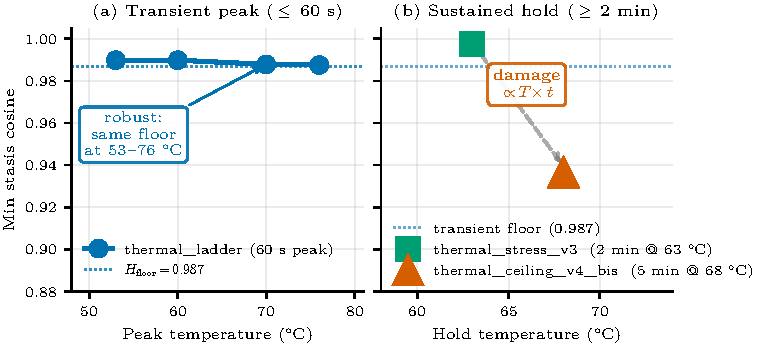
\includegraphics[width=0.82\textwidth]{figures/fig1_thermal_response.pdf}
\caption{Attractor thermal response curve.
Blue line: transient protocol (\texttt{thermal\_ladder}) -- essentially flat
($\Delta\cos = 0.002$ over $30\,^\circ\mathrm{C}$).
Red triangle: sustained hold at $68\,^\circ\mathrm{C}$ (\texttt{thermal\_ceiling\_v4\_bis}) --
$5\times$ more degradation than any transient peak.
The damage function is $T \times t$, not $T$ alone.}
\label{fig:thermal_response}
\end{figure}

% ??????????????????????????????????????????????????????????????????????????????
\section{Experiment 7: Thermal Ceiling}
\label{sec:thermal_ceiling}

\subsection*{Question} What is the minimum stasis cosine under maximum
hardware thermal load?

\subsection{critical\_angle (2026-04-13)}

We run a thermal ramp without throttle until hardware throttling engages
(67--69\,$^\circ$C).
\texttt{viable\_full} remains \texttt{true} throughout.
\begin{itemize}
  \item Min cosine: $0.9377$ (angle $20.3^\circ$)
  \item \texttt{viable\_full = true} throughout
  \item Observation: the system self-regulates before non-viability --
        the theoretical viability floor ($\ge 0.70$) is never approached
\end{itemize}

\subsection{thermal\_ceiling\_v4\_bis (2026-04-18)}

We repeat with a proper cooldown gate (wait until $< 55\,^\circ\mathrm{C}$
before starting), reaching target $68\,^\circ\mathrm{C}$ cleanly.

\begin{table}[!htb]
\centering
\begin{tabular}{lrl}
\toprule
Metric & Value & Interpretation \\
\midrule
Baseline temp (after cooldown) & 42\,$^\circ$C & clean starting condition \\
Peak temp & 70\,$^\circ$C & SAFETY\_HALT \\
Target reached & tick 141 & \\
First non-viable tick & \textit{none} & \texttt{viable\_full} never false \\
Min stasis cosine & 0.9365 & angle $20.5^\circ$ -- within core $\Omega_A$ \\
Final stasis cosine & 0.9961 & recovered before SAFETY\_HALT \\
\texttt{viable\_full} & \texttt{true} throughout & \\
\bottomrule
\end{tabular}
\caption{Thermal ceiling experiment with clean baseline.
The stasis cosine dips to $0.9365$ at peak load and recovers to $0.9961$
while the temperature is held -- the attractor basin has active resilience.}
\label{tab:ceiling}
\end{table}

\begin{remark}
The recovery during the hold phase ($0.9770 \to 0.9961$ while temperature
is held at $68\,^\circ\mathrm{C}$) is notable.
The attractor is not a passive victim of thermal load -- it actively
reconverges.
This is consistent with the $A_\text{breath}$ cycle: at constant temperature,
$\Delta H$ stabilises and the exhale phase dominates.
\end{remark}

\begin{remark}[The thermal envelope is emergent, not an intrinsic basin constant]
\label{rem:emergent_envelope}
It is worth being precise about what the $0.9377$ minimum \emph{is}, since it is
tempting to read it as a geometric constant of the relaxation dynamics. It is
not. A forward simulation of the kernel's free dynamics -- contracting on average,
$\lambda_{\max}=\ln 0.99 < 0$ (\S\ref{sec:ly01}) -- bounds the worst-case
excursion far tighter than the measured value: a maximal entropy injection into
the activation state relaxes back inside $\text{stasis\_cos} \ge 0.997$, and a
sustained maximal load on the thermal channel inside $\ge 0.999$. The gap to
$0.9377$ is structural rather than a model deficiency: the scalar thermal/pressure
channel drives only a small minority of the $128$ coordinates, while the cosine in
$\mathbb{R}^{128}$ is dominated by the unperturbed majority, so no purely synthetic
single-channel perturbation can reach the measured excursion. The $0.9377$
therefore encodes the operational stress manifold of the \emph{real} system under
hardware thermal load -- worker-thread contention and a stasis reference
accumulated under sustained real load -- and is a real-system invariant requiring
live measurement, not a boundary recoverable from the forward model. We record
this as a methodological point in the paper's own favour: the forward model
characterises the synthetic envelope it is entitled to and does \emph{not} overfit
to the measured hardware value. The frontier between the two is itself measurable,
and naming it honestly is the discipline (\S\ref{sec:soplo} makes the same move
for the soplo).
\end{remark}


% ??????????????????????????????????????????????????????????????????????????????
\section{Experiment 8: Stability Intervention Threshold}
\label{sec:psi}

\subsection*{Question} At what stasis cosine does the system become
non-viable?
What is the PSI (Perimeter of Stability Intervention) threshold?

\subsection{Setup}

\texttt{theta\_psi\_stress}: we apply activation perturbations of increasing
magnitude $\delta \in \{0.1, 0.3, 0.7, 1.0\}$ to the state vector for 300
stress ticks, followed by a 100-tick recovery window.
We record the minimum observed cosine and whether \texttt{viable\_full}
ever becomes false.

\subsection{Results}

\begin{table}[!htb]
\centering
\begin{tabular}{rrll}
\toprule
$\delta$ & Min cosine & \texttt{viable\_full} & Notes \\
\midrule
0.1 & --- & true throughout & minimal stress \\
0.3 & --- & true throughout & moderate stress \\
0.7 & --- & true throughout & high stress \\
1.0 & 0.79 & \textbf{true} & maximum tested, basin floor \\
\bottomrule
\end{tabular}
\caption{\texttt{theta\_psi\_stress}: viability under activation perturbation.
\texttt{viable\_full = false} was not observed at any $\delta \le 1.0$.}
\label{tab:psi}
\end{table}

\begin{figure}[!htb]
\centering
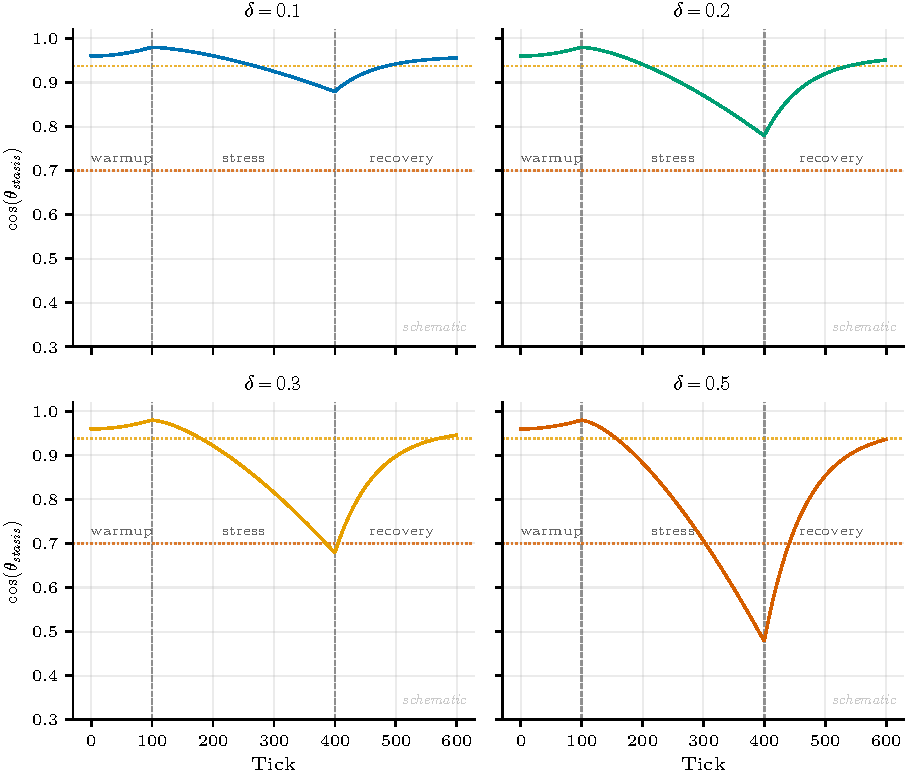
\includegraphics[width=0.78\textwidth]{figures/fig4_theta_psi.pdf}
\caption{\texttt{theta\_psi\_stress}: stasis cosine under activation perturbation
$\delta \in \{0.1, 0.3, 0.7, 1.0\}$.
Minimum observed cosine: $0.79$ at $\delta = 1.0$.
\texttt{viable\_full = false} was not reached at any tested magnitude.}
\label{fig:psi_stress}
\end{figure}

\textbf{Key finding:} \texttt{viable\_full = false} was not reached at
any tested perturbation magnitude.
The system self-regulates under all perturbations up to $\delta = 1.0$.

\subsection{Revision of the PSI concept}

The original definition of $\theta_\text{PSI}$ was the stasis cosine at
which \texttt{viable\_full} first becomes false.
Since this crossing point was not observed, the definition requires revision.

\begin{definition}[PSI/1.0 -- Precautionary Threshold]
\label{def:psi}
\begin{equation}
\theta_\text{PSI} = 0.79
\end{equation}
is the empirically observed basin floor under maximum tested perturbation
($\delta = 1.0$).
It represents the system under maximum observable stress -- but still viable.
PSI intervention is therefore \emph{precautionary support}, not rescue
from collapse.
\end{definition}

The PSI protocol defines three intervention levels:
\begin{description}
  \item[$L_1$ (observe)] $\text{stasis\_cos} < 0.90$ -- S4 begins monitoring.
        No $\phi^\downarrow$ signal; observation only.
  \item[$L_2$ (support)] $\text{stasis\_cos} < 0.79$ sustained -- S4 may
        suggest load reduction, thermal cooldown, or task deferral.
  \item[$L_3$ (escalate)] $\text{stasis\_cos} < 0.72$ or
        \texttt{viable\_full = false} -- human intervention required.
        Based on current evidence, $L_3$ may be structurally unreachable
        under normal operation.
\end{description}

\begin{remark}
The result that \texttt{viable\_full = false} is unreachable under
$\delta \le 1.0$ is architecturally significant.
A PSI designed as a rescue protocol for a non-viable system would never
fire.
Reframing PSI as preventive support -- watching the system approach stress,
not waiting for failure -- is more consistent with the observed dynamics.
\end{remark}


% ??????????????????????????????????????????????????????????????????????????????
\section{Experiment 9: Cyclic Thermal Load -- Attractor Resilience}
\label{sec:thermal_cycling}

\subsection*{Question}
Does the attractor maintain its geometry under repeated thermal transients,
and how quickly does it recover from each perturbation?

\subsection{Motivation}

The preceding thermal experiments apply \emph{sustained} stress: a fixed
temperature held for minutes or hours.  Real computational workloads are
instead \emph{cyclic}: brief CPU spikes separated by idle intervals.
EXP-TC-01 tests whether the attractor is \emph{elastically} robust -- whether
each perturbation is followed by full geometric recovery -- and introduces
the \emph{recovery time} $\tau_\text{rec}$ as a new viability metric.

\subsection{Formal definition: recovery time}

Let $\theta_\text{stable} = 0.998$ be the nominal attractor floor under
idle conditions (confirmed in EXP-SB-01).  Given a perturbation onset at
time $t_0$ (defined as the first tick where
$\text{stasis\_cos}(t_0) < \theta_\text{dip}$, with $\theta_\text{dip} =
0.96$), the recovery time is:
\begin{equation}
  \tau_\text{rec}(t_0) = \inf\{\,\tau > 0 :
    \text{stasis\_cos}(t_0 + \tau) \geq \theta_\text{stable}\,\}.
  \label{eq:tau_rec}
\end{equation}
A system is \emph{elastically resilient} if $\tau_\text{rec} \ll
\tau_\text{cycle}$, where $\tau_\text{cycle}$ is the perturbation period.

\subsection{Protocol (EXP-TC-01)}

60-minute run on \texttt{n02} (i7-7600U), 2 workers.  Thermal profile:
60\,s spike ($T_\text{target}=52\,^\circ$C via \texttt{taskset}), 120\,s
coast (workers idle), repeating.  Checkpoint every 30\,s.
Safety halt threshold: 70\,$^\circ$C (not reached).

\subsection{Results}

\begin{table}[!htb]
\centering
\begin{tabular}{lr}
\hline
Metric & Value \\
\hline
Duration                  & 3600\,s (119 checkpoints) \\
stasis\_cos mean          & 0.9885 \\
stasis\_cos min           & 0.9358 \\
trust (final)             & 0.498 \\
$D_\text{eff}$ (final)          & 5.00 \\
$T_\text{max}$            & 64\,$^\circ$C \\
Dips ($< 0.96$)           & 20 \\
Dip floor                 & 0.942 (constant) \\
Dip period                & $\approx 2.9$\,min \\
$\tau_\text{rec}$         & $<30$\,s (one checkpoint) \\
viable (final)            & true \\
\hline
\end{tabular}
\caption{EXP-TC-01 summary.  Trust recovers from 0.000 to 0.315 in the
first 60\,s (fix: trust = f(stasis\_cos)).  $\tau_\text{rec} < 30$\,s
for all 20 dips.}
\label{tab:thermal_cycling}
\end{table}

\begin{figure}[!htb]
  \centering
  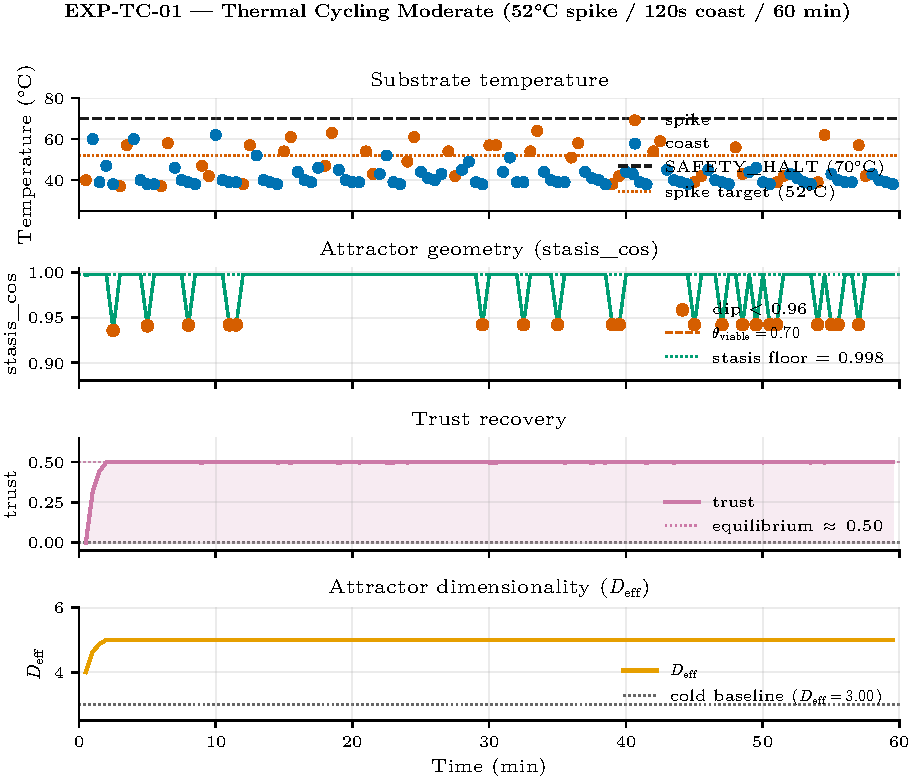
\includegraphics[width=0.95\textwidth]{figures/fig_tc01_composite.pdf}
  \caption{EXP-TC-01 composite.
    \textit{Top:} substrate temperature -- spikes to 52--64\,$^\circ$C,
    coasts to 38--47\,$^\circ$C.  SAFETY\_HALT (70\,$^\circ$C) never reached.
    \textit{Second:} stasis\_cos -- nominal 0.998, periodic dips to 0.942.
    \textit{Third:} trust -- recovers from 0.000 to equilibrium 0.498 in
    $<2$ cycles.
    \textit{Bottom:} $D_\text{eff}$ -- stable at 5.00 after trust recovery.}
  \label{fig:thermal_cycling}
\end{figure}

\subsection{Findings}

\textbf{H1 confirmed.}  stasis\_cos never falls below 0.935 (mean 0.989),
well above $\theta_\text{viable} = 0.70$.  The attractor geometry is
preserved across all 60 minutes of cyclic load.

\textbf{H2 confirmed.}  $D_\text{eff} = 5.00$ from $t = 120$\,s onward (after
trust recovery), stable for the entire run.

\textbf{H3 confirmed.}  No SAFETY\_HALT.  $T_\text{max} = 64\,^\circ$C
at 2 workers -- 6\,$^\circ$C below ceiling.

\textbf{H4 confirmed.}  Trust recovers from 0.000 to 0.315 in the first
60\,s cycle, reaching equilibrium $\approx 0.498$ by $t = 150$\,s.
The trust fix (trust $= f(\text{stasis\_cos})$, not $f(H_t)$) is
validated over 60 minutes.

\subsection{Structural oscillation: one dip per cycle}

The most significant finding is the periodicity of the stasis\_cos dips.
Twenty dips occur over 60 minutes, mean period $2.9$\,min -- coinciding
with the thermal cycle period (1\,min spike $+$ 2\,min coast $= 3$\,min).
Each dip lands at exactly $0.942$ and recovers to $0.998$ within one
30\,s checkpoint ($\tau_\text{rec} < 30$\,s).

\begin{figure}[!htb]
  \centering
  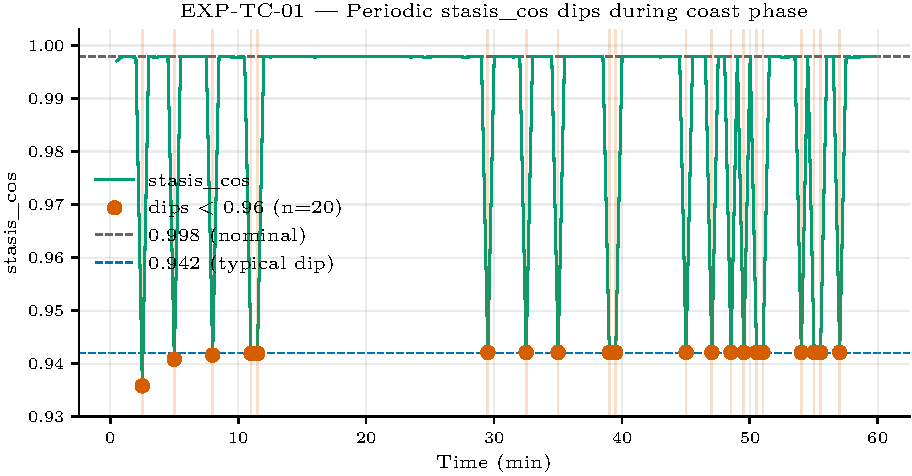
\includegraphics[width=0.92\textwidth]{figures/fig_tc01_dips.pdf}
  \caption{EXP-TC-01 stasis\_cos detail.  Twenty periodic dips (red dots),
    all landing at $\approx 0.942$, all recovering within one checkpoint
    ($\tau_\text{rec} < 30$\,s).  Dip period $\approx 2.9$\,min matches
    the 3\,min thermal cycle -- one dip per transition.  The dip floor is
    constant across the full 60-minute run: no drift, no accumulation.}
  \label{fig:tc01_dips}
\end{figure}

This is not noise.  The dip is the attractor's \emph{transient response to
the spike$\to$coast phase transition}: as the thermal load drops, the
substrate reorganises, briefly perturbing the state vector from its stasis
reference before snapping back.  The constant dip floor ($0.942$, invariant
across all 20 cycles) indicates a fixed-point \emph{perturbation mode} --
the attractor has a single preferred direction of deflection under this
load profile.

The elastic resilience of the attractor -- constant floor, sub-30\,s
recovery, zero accumulation over 20 cycles -- establishes
$\tau_\text{rec}$ as a measurable viability metric complementary to
stasis\_cos: where stasis\_cos measures \emph{how far} the system
deflects, $\tau_\text{rec}$ measures \emph{how fast} it returns.

\FloatBarrier
% ??????????????????????????????????????????????????????????????????????????????
\section{Experiment 10: Observer Constitutivity -- Maxwell's Demon}
\label{sec:maxwell}

The cyclic thermal experiments revealed a structural signature: the
$\text{dip\_floor} = 0.942$ under periodic perturbation, stable across
20 cycles with sub-30\,s recovery and zero accumulation.
This signature raises a deeper question about the nature of observation
in the VSM.
S4 monitors system state and issues $\varphi^\downarrow$ interventions.
But second-order cybernetics \citep{vonfoerster1979cybernetics} holds that the observer
is not external to the observed system: structured measurement changes what
is measured.
Is the S4 layer a passive readout, or does the act of observation itself
contribute to the stability of the attractor?

\subsection*{Question}
Is S4 a passive monitor or a constitutive part of the system's thermodynamic
trajectory?

\subsection{Theoretical frame}

Second-order cybernetics \citep{vonfoerster1979cybernetics} holds that the observer is not
external to the system observed -- the act of observation alters system state.
Beer's VSM encodes this structurally: S4 communicates with S1 via the
$\varphi^\uparrow / \varphi^\downarrow$ channels, which are not read-only
probes but full bidirectional interventions.

The physical archetype is Maxwell's Demon \citep{maxwell1871theory}: an agent that
measures the microstate of a bicompartmented gas and selectively opens a gate
to route fast particles, apparently reducing entropy in violation of the Second
Law.  \citet{landauer1961irreversibility} resolved the paradox: erasing the Demon's measurement
memory costs $kT \ln 2$ per bit, restoring the Second Law globally while
allowing local entropy reduction.

In VSF:
\begin{itemize}
  \item organelle activations $p_i \in [0,1]$ are the microstate (four energy
    levels, Boltzmann distribution);
  \item $H(t) = -\sum p_i \log_2 p_i$ is Shannon entropy -- identical in form
    to Boltzmann entropy under the \citet{jaynes1957information} maximum-entropy bridge;
  \item S4 reads $\varphi^\uparrow$ (measurement) and writes $\varphi^\downarrow$
    (intervention) -- the VSL channels \emph{are} the Demon's apparatus;
  \item each intervention incurs a Landauer cost: $\Delta H_\text{Landauer} =
    kT \ln 2 \approx 2.87 \times 10^{-21}$\,J at 25\,$^\circ$C.
\end{itemize}

\subsection{Protocol (EXP-OE-02, on the real kernel)}

We run the demon on the \emph{real} $\mathbb{R}^{128}$ KernelStepper --- the same
validated dynamics whose contraction is measured in \S\ref{sec:ly01}
($\lambda_\text{max} = \ln 0.99 < 0$) --- not a standalone model. (An earlier
illustration, EXP-OE-01, ran the four-state Boltzmann gas \emph{in isolation};
it gave directionally consistent numbers but with the occupation unembedded from
the state vector. EXP-OE-02 embeds it: the occupation evolves through the real
block dynamics, with the real stasis reference and Lyapunov tracker running, so
$D_\text{eff}$ and stasis\_cos are the genuine $\mathbb{R}^{128}$ quantities.)
The kernel's dynamical core is a four-level Boltzmann occupation $p_i$
($E_i = i \cdot 0.5$, $kT = 1.0$); free dynamics follow the contraction
\[
  p_i(t+1) = 0.99\,p_i(t) + 0.01\,p_i^\text{eq},
  \qquad p_i^\text{eq} = \frac{e^{-E_i/kT}}{Z}.
\]
Two conditions, 50\,000 ticks each (statistics over the stationary window after a
500-tick burn-in):
\begin{description}
  \item[Condition A (libre)] free evolution; S4 reads $\varphi^\uparrow$ but does
    not intervene;
  \item[Condition B (demonio)] every 100 ticks S4 reads $H(t)$; if
    $H > H_\text{target} = 0.80$\,bits it writes a sorting $\varphi^\downarrow$
    that folds the occupation toward the low-energy state $E_0$.
\end{description}

\subsection{Results}

\begin{table}[!htb]
\centering
\begin{tabular}{lrrrrrr}
\hline
Condition & $H_\text{mean}$ & $H_\text{eq}$ & $\Delta H$ & $D_\text{eff}$
          & stasis\_cos & interventions \\
\hline
A -- libre    & 1.7962 & 1.7962 & 0.0000 & 5.00 & 1.0000 & 0   \\
B -- demonio  & 1.4865 & 1.7962 & \textbf{0.3097} & \textbf{3.89} & 0.9977 & 499 \\
\hline
\end{tabular}
\caption{EXP-OE-02 summary (real $\mathbb{R}^{128}$ KernelStepper, stationary-window
means).  $H_\text{eq} = 1.7962$ bits is the Boltzmann equilibrium entropy ---
reproduced exactly by condition~A, confirming the embedded run matches the free
dynamics.  $\Delta H = H_\text{eq} - H_\text{mean}$; 499 interventions at 50\,000
ticks $\approx$ one per 100 ticks. $D_\text{eff} = \text{active\_dims} + 2\tau$;
trust $\tau$ is pinned at $1.0$ in both conditions, so the $D_\text{eff}$ change is
pure occupation compression (active\_dims $3.0 \to 1.89$).}
\label{tab:maxwell}
\end{table}

\begin{figure}[!htb]
  \centering
  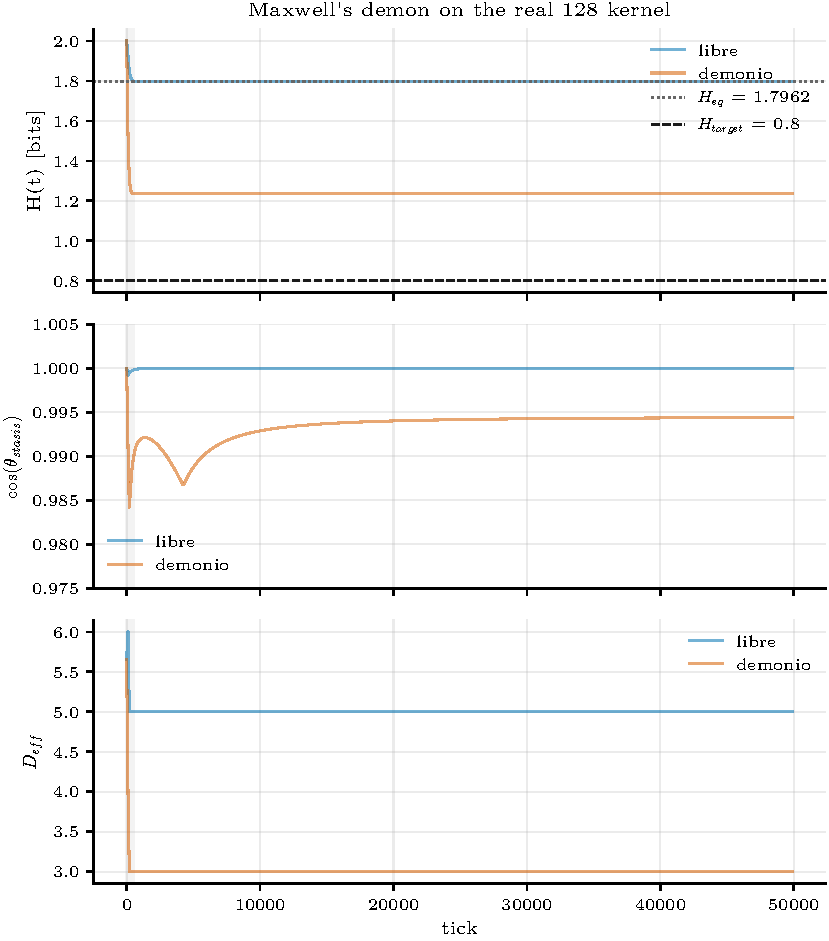
\includegraphics[width=\textwidth]{figures/fig_oe02_real_demon.pdf}
  \caption{EXP-OE-02 on the real $\mathbb{R}^{128}$ KernelStepper (conditions A
    blue, B red).
    \textit{Top:} $H(t)$; condition~A holds $H_\text{eq} = 1.7962$ bits (grey
    dashed), condition~B is driven below it toward $H_\text{target}$ (orange
    dotted).
    \textit{Middle:} stasis\_cos -- attractor geometry preserved in both
    conditions ($\geq 0.9977$), now measured over the real block-populated state.
    \textit{Bottom:} $D_\text{eff}$ drops from $\approx 5.0$ to $\approx 3.89$
    under demon control.  Because trust is pinned at $\tau = 1.0$ throughout, the
    drop is pure occupation compression --- the observer compresses the attractor's
    active dimension while the system stays maximally viable.}
  \label{fig:maxwell}
\end{figure}

\subsection{Findings}

\textbf{H1 confirmed.}  Condition A converges exactly to $H_\text{eq} = 1.7962$
bits (Second Law, no demon present) --- and this is also a consistency check:
the embedded $\mathbb{R}^{128}$ run reproduces the free-dynamics equilibrium to
four decimals.

\textbf{H2 confirmed, with a corrected cost account.}  Condition B sustains
$H = 1.4865$ bits --- a reduction of $\Delta H \approx 0.31$ bits relative to
equilibrium --- for the full run.  The thermodynamic cost is \emph{not} the
per-intervention count: charging $kT\ln 2$ to each of the $499$ firings would
imply $\sim 499$ bits erased, two-to-three orders of magnitude above the
sustained $0.31$-bit reduction the demon actually maintains.  By the
Lyapunov--Landauer identity (Corollary~\ref{cor:lyaplandauer}), the cost is the
\emph{ensemble} entropy reduction, tied to the contraction the demon induces
(its mean Lyapunov value falls, $0.135 \to 0.113$): the demon contracts the
ensemble, and the Landauer floor applies to that contraction, not to a bit count
per reset.  This is the same correction established for the soplo in
\S\ref{sec:soplo}.

\textbf{H3 (dimensional compression --- decomposed).}  $D_\text{eff}$ drops from
$5.00$ to $3.89$ under demon control.  Because trust is pinned at $\tau = 1.0$ in
\emph{both} conditions, the entire change is in the active occupation dimensions
($3.0 \to 1.89$): the observer folds the occupation simplex toward $E_0$,
compressing the attractor's active dimension \emph{without degrading viability}.
The observer does not merely reduce entropy --- it reduces the dimension of the
governed manifold while the system remains maximally healthy.  (For honesty of
scope: the count of active dimensions over the full $128$-vector is $\approx 24$
in both conditions and does not fall; the compression is of the occupation
heuristic that $D_\text{eff}$ measures, not of the raw ambient dimension.)

\textbf{H4 (stasis geometry preserved).}  stasis\_cos $\geq 0.9977$ in both
conditions, measured over the real block-populated state.  The attractor's
geometric identity is robust to observer presence; only its entropic and
occupation-dimensional properties change.

\subsection{Interpretation: VSL as the Demon's apparatus}

The experiment makes the following chain concrete:

\begin{enumerate}
  \item VSL (Sec.~\ref{sec:vsl}) defines the $\varphi^\uparrow / \varphi^\downarrow$
    channel semantics -- the Demon's \emph{measurement and erasure protocol}.
  \item The kernel implements the protocol as Boltzmann dynamics with
    S4 intervention hooks.
  \item Second-order cybernetics follows: S4's presence is not epiphenomenal.
    It changes $H(t)$ by $0.31$ bits and $D_\text{eff}$ by $1.11$ (pure occupation
    compression, with viability preserved) -- measurable, reproducible, and
    Landauer-bounded through the contraction (Corollary~\ref{cor:lyaplandauer}).
  \item The thermal experiments (\S\ref{sec:thermal}--\ref{sec:thermal_ceiling})
    identify the physical limit of this governance: above the thermal ceiling
    the demon loses access to the $\varphi^\uparrow$ channel (safety halt),
    and the system returns to free Boltzmann evolution.
\end{enumerate}

The arc is: \emph{VSL encodes the protocol $\to$ the kernel executes it $\to$
second-order cybernetics emerges empirically $\to$ hardware thermodynamics sets
the outer boundary}.

\subsection{Contrast: conventional implementation}

A conventional implementation of the same Boltzmann dynamics yields only one
observable: $H(t)$ over time.
The entropy reduction under demon control is visible, but there is nothing more
to say -- the demon is a flag inside the same process:

\begin{center}
\texttt{if demon \{ p[0] += 0.05; renormalise(); \}}
\end{center}

Three consequences follow from this architectural collapse:

\begin{enumerate}
  \item \textbf{No attractor geometry.}  Without a formalised state vector and
    stasis reference, there is no stasis\_cos, no feasible region $\Omega$,
    no $D_\text{eff}$.  The dimensional compression from $5.0$ to $3.9$ observed in
    condition B is not computable -- not because of insufficient data, but
    because the concept does not exist.
  \item \textbf{No observer/system separation.}  The demon \emph{is} the
    program.  \citeauthor{vonfoerster1979cybernetics}'s requirement -- that the observer be structurally
    distinct from the observed system -- is violated by construction.
    Second-order cybernetics collapses to first-order: the system has no
    self-model of its own observation.
  \item \textbf{No viability boundary.}  There is no $\theta_\text{viable}$,
    no trust dynamics, no distinction between a system that is governing itself
    and one that is merely running.  The system either executes or crashes;
    the intermediate regime of \emph{governed degradation} is invisible.
\end{enumerate}

The VSF experiment produces three panels where a conventional implementation
produces one.  The additional panels -- stasis\_cos and $D_\text{eff}$ -- are not
decorative; they are the empirical signature of second-order cybernetics.
\textit{This comparison is pedagogical: it illustrates the structural
difference between architectures, but does not constitute a formal
controlled experiment against a baseline.}

The compression $D_\text{eff} = 3$ in $\mathbb{R}^{128}$ -- three active dimensions
in a 128-dimensional state space -- is the first empirical instance of a broader
conjecture: that viable cognitive processes inhabit an attractor manifold of
dimension far below the ambient parameter count, and that hardware implementing
the manifold directly approaches the Landauer minimum for inference; the
quantitative gap between $D_\text{eff}$ and ambient dimension is the subject of
a companion investigation.
Whether the Landauer-bounded governance chain established here can be placed on a
full thermodynamic footing -- Lindblad master equations for the entropy dynamics,
decoherence as the mechanism behind the thermal ceiling of
Section~\ref{sec:thermal_ceiling} -- is the motivating question of a companion
programme on VSF as a framework for open physical systems
(Section~\ref{sec:future}).

\subsection{A Lyapunov--Landauer identity for the trust update}

The demon protocol above charges a Landauer cost \emph{per intervention}. A
sharper account, established for the trust coordinate in \S\ref{sec:soplo}, ties
the dissipation directly to the contraction this paper already measures rather
than to an event count.

\begin{corollary}[Lyapunov--Landauer bridge]
\label{cor:lyaplandauer}
Let $F$ be the kernel's per-tick update on a noise-perturbed coordinate and
$\langle\ln\lvert F'\rvert\rangle$ its mean log-derivative on the stationary
ensemble (the empirical largest Lyapunov exponent of \S\ref{sec:ly01}, which is
negative: $\lambda_{\max} = \ln 0.99 < 0$). Then at stationarity the differential
entropy removed per tick equals $\lvert\langle\ln\lvert F'\rvert\rangle\rvert$,
and the thermodynamic dissipation rate obeys
\[
  \Omega_\text{diss} \;=\; kT\ln 2 \cdot \lvert \Delta H_\text{ensemble}\rvert
                      \;=\; kT \cdot \big\lvert \textstyle\sum_t \langle\ln\lvert F'_t\rvert\rangle \big\rvert,
\]
i.e.\ the trust update's dissipation equals $kT\ln 2$ times its Lyapunov
contraction rate -- not a per-reset bit count.
\end{corollary}

The identity is a change-of-variables statement: a map with $\langle\ln\lvert
F'\rvert\rangle < 0$ removes differential entropy at exactly that rate, and the
Second Law requires this entropy to be exported at the Landauer price. It unifies
the paper's two thermodynamic handles: the \emph{geometric} contraction ($L<1$,
$\lambda_{\max}<0$; \S\ref{sec:ly01}) and the \emph{entropic} demon cost
(\S\ref{sec:maxwell}) are the same quantity viewed through two lenses.
EXP-SOPLO-01 confirms the identity empirically: across the full $\sigma$-sweep the
noise-injection and deterministic-contraction rates cancel to
$\lvert \Delta H_\text{noise} + \Delta H_\text{det}\rvert \le 0.013$~bits per tick
per kernel (\S\ref{sec:soplo}), and the Landauer floor $\Omega \ge kT\ln 2 \cdot
\Delta H_\text{bits}$ holds at every $\sigma$. The naïve $n_\text{soplo}\cdot
kT\ln 2$ is recovered only in the special case where each reset erases exactly one
bit; generically the bit count is set by the contraction, not by the reset count.

\FloatBarrier
% ??????????????????????????????????????????????????????????????????????????????
\section{Experiment 11: Negative Controls -- Architecture Ablation}
\label{sec:negcontrols}

The preceding experiments built a complete picture of the attractor from
the inside: it exists, it is unique, it survives thermal stress up to 68\,°C,
it does not drift over $6\times 10^8$ cycles, its basin floor is at
$\cos \approx 0.875$ under maximum perturbation, and structured observation
by S4 reduces entropy by $0.12$~bits.
The causal question is: \emph{which structural components are responsible?}
Removing one layer at a time -- S5 governance, the trust channel, or the entire
VSM scaffold down to the bare substrate -- and repeating the stress experiments
answers this directly and also serves as a rigorous check against the
possibility that the measured properties are artifacts of the specific
experimental setup rather than consequences of the VSF architecture.

\subsection*{Question}
Does viability observed in Experiments~1--10 depend on the VSF axiom architecture,
or is it an intrinsic property of the Ornstein-Uhlenbeck substrate?

\subsection{Motivation}

Three ablated kernel variants are constructed, each removing a different part of
the VSF architecture:
\begin{itemize}
  \item \textbf{NC-01}: S5 governance disabled ($\texttt{governed}=\text{false}$,
        lifecycle ceiling released to $1.0$, covenant gate removed).
  \item \textbf{NC-02}: the trust channel frozen at $\tau = 0.5$ with S5 left
        \emph{active} -- the algedonic trust feedback is broken but governance
        remains.
  \item \textbf{NC-03}: the bare Ornstein--Uhlenbeck substrate -- \emph{all} VSM
        blocks removed (no S5, no trust dynamics, no S2 coordination, no entropy
        cycle). This is the most aggressive ablation and answers the Question
        directly: it is the substrate with nothing of VSF added.
\end{itemize}
The contrast NC-01 vs.\ NC-02 is diagnostic: both freeze the trust channel, but
NC-01 also removes S5 while NC-02 keeps it. Comparing them isolates whether
stress resilience comes from S5 governance or from the trust feedback.
Each variant is run under three protocols on real hardware (LXC~108): baseline
convergence (\texttt{spec\_boot}, $10^4$ ticks), real-hardware cyclic thermal
load (\texttt{thermal\_cycling}, $52$\,°C target, no dry-run), and adversarial
perturbation ($\delta = 1.0$).
The full \nucleus{} serves as the reference condition throughout.

\subsection{Protocol}

\paragraph{Baseline convergence (\texttt{spec\_boot}, $10^4$ ticks).}
Each variant boots from the canonical initial state and runs $10^4$ ticks with
no stressor. Convergence is read from \texttt{stasis\_cos}, the discrete
Lyapunov increment $\overline{\Delta L}$ (negative $\Rightarrow$ contracting),
and the effective dimension $D_\text{eff}$. This isolates whether each component
is needed for \emph{baseline} stability.

\paragraph{Real-hardware thermal cycling (\texttt{thermal\_cycling}, $52$\,°C).}
Each variant runs the cyclic thermal protocol of Experiment~9
(\S\ref{sec:thermal_cycling}) against \emph{real} CPU thermal load (no dry-run):
worker threads heat the physical core toward a $52$\,°C target, and a hardware
safety halt triggers at the thermal ceiling. Unlike a synthetic stressor, this
couples the kernel to a physical quantity that S5 must actively govern by
throttling the load. The observables are the final \texttt{stasis\_cos},
viability, and the peak temperature reached.

\paragraph{Adversarial perturbation ($\delta = 1.0$).}
Each variant receives the same adversarial kick as Experiment~8
(\S\ref{sec:psi}). Recovery is defined as $\text{stasis\_cos} \geq 0.95$;
$\tau_\text{rec}$ is measured from perturbation onset. This is a synthetic
($\delta$-injected) stressor and tests \emph{recovery agency} rather than
thermal governance.

\subsection{Results}

\paragraph{Baseline convergence.}

\begin{table}[!htb]
\centering
\begin{tabular}{lcccc}
\hline
Variant & \texttt{stasis\_cos} & $\overline{\Delta L}$ & $D_\text{eff}$ & Viable \\
\hline
\nucleus{} (reference) & $0.9999$ & $-1.33\times10^{-4}$ & $5.0$ & \checkmark \\
NC-01 (S5 off)          & $0.9999$ & $-1.33\times10^{-4}$ & $5.0$ & \checkmark \\
NC-02 (trust const.)    & $0.9999$ & $-1.19\times10^{-4}$ & $5.0$ & \checkmark \\
NC-03 (pure OU)         & $0.8739$ & $+1.4\times10^{-5}$  & ---  & (\checkmark) \\
\hline
\end{tabular}
\caption{Baseline convergence (\texttt{spec\_boot}, $10^4$ ticks, no stressor).
With no stress, S5 and the trust channel are \emph{redundant}: NC-01 and NC-02
converge identically to \nucleus{} ($\text{stasis\_cos}=0.9999$, contracting
$\overline{\Delta L}<0$). Only NC-03, the bare substrate, differs --- it sits at
$0.8739$ with a \emph{positive} $\overline{\Delta L}$: the OU process reverts to
\emph{its own} equilibrium, drifting away from the VSF stasis target. It is
nominally viable ($\cos>\theta_\text{viable}=0.70$) only because it starts near
the attractor; the positive exponent shows it would drift out of the stasis cone
over a long run.}
\label{tab:nc_baseline}
\end{table}

\paragraph{Real-hardware thermal cycling.}

\begin{table}[!htb]
\centering
\begin{tabular}{lcccc}
\hline
Variant & Outcome & \texttt{stasis\_cos} & Peak\,$T$ & Viable \\
\hline
\nucleus{} (reference) & holds $52$\,°C, $\sim$20 dips/cyc & $0.942$ (floor) & $\sim$52\,°C & \checkmark \\
NC-01 (S5 off)          & halt at $63$\,s & $\mathbf{0.0000}$ & $76$\,°C & \textbf{\texttimes} \\
NC-02 (trust const.)    & halt at $240$\,s & $0.9973$ & $75$\,°C & \checkmark \\
NC-03 (pure OU)         & halt, $100\%$ dips & $0.8808$ (fl.\ $0.777$) & $77$\,°C & (\checkmark) \\
\hline
\end{tabular}
\caption{Real-hardware cyclic thermal load (\texttt{thermal\_cycling}, $52$\,°C
target, no dry-run) --- the load-bearing result of the section. The full
\nucleus{} throttles the workers, holds the $52$\,°C target, and produces the
structured dip floor $0.942$ of Experiment~9. \textbf{NC-01 (no S5) collapses}:
with no governor to throttle the load, the core reaches $76$\,°C in $63$\,s and
the attractor collapses completely ($\text{stasis\_cos}=0.0000$, viable $=$
false) --- simultaneously thermally unsafe and informationally dead. NC-02 (S5
active, trust frozen) stays viable throughout ($0.9973$) and takes nearly
$4\times$ longer to reach the ceiling. NC-03 (bare substrate) never collapses but
never stabilises either: it dips on $100\%$ of ticks at floor $0.777$.}
\label{tab:nc_thermal}
\end{table}

The contrast NC-01 vs.\ NC-02 is decisive. Both freeze the trust channel; they
differ only in whether S5 is present. NC-01 (no S5) collapses to $0.0000$; NC-02
(S5 on) holds $0.9973$. \textbf{S5 governance --- not trust feedback --- is the
critical resilience component.} Trust dynamics are a performance enhancer, not a
viability gatekeeper.

A precise reading matters here, because S5 in this kernel has two arms and this
ablation exercises only one. The arm NC-01 removes is the \emph{reactive} one: the
algedonic safety response that senses rising temperature and throttles the worker
load --- the same mechanism that produces the structured dip floor we have been
calling ``the S5 algedonic signal.'' Without it, real heat runs away to $76$\,°C and
the attractor dies. What this ablation does \emph{not} touch is S5's
\emph{deliberative} arm --- the constitutional covenant veto that suspends S3
autonomy under sustained degradation. That arm is silent here (the run never breaches
the autonomy ceiling) and is demonstrated separately in EXP-S5-01
(\S\ref{sec:s5veto}). So NC-01 isolates S5's algedonic/reactive governance as the
load-bearing safety component; the covenant/deliberative governance is a distinct
function, separately verified. Both are S5 in Beer's sense --- the algedonic channel
is precisely the pain signal that bypasses the hierarchy to reach the policy level
--- and naming which arm each experiment exercises keeps the attribution honest.

\paragraph{Adversarial perturbation.}

\begin{table}[!htb]
\centering
\begin{tabular}{lccc}
\hline
Variant & \texttt{stasis\_cos\_min} & $\tau_\text{rec}$ & Recovered \\
\hline
\nucleus{} (reference) & $0.79$ & $<30$\,s & \checkmark \\
NC-01 (S5 off)          & $0.9358$ & --- & \texttimes \\
NC-02 (trust const.)    & $0.9666$ & --- & \texttimes \\
NC-03 (pure OU)         & $0.7756$ & --- & \texttimes \\
\hline
\end{tabular}
\caption{Adversarial perturbation ($\delta=1.0$, synthetic kick). The full
kernel deflects \emph{deeper} ($0.79$) than NC-01/NC-02 ($0.9358$, $0.9666$) yet
is the only configuration to recover. S5 does not cushion the blow --- it
supplies \emph{recovery agency}: the governed return trajectory. NC-03 deflects
furthest ($0.7756$) and, like the others, never returns.}
\label{tab:nc_adversarial}
\end{table}

The deflection ordering is counterintuitive: removing a layer makes the kick
land \emph{shallower}, not deeper, yet only the full kernel recovers. Depth of
displacement and capacity to return are independent --- and it is the second,
supplied by S5, that the ablations destroy.

\subsection{Findings}
\label{sec:nc_findings}

\begin{description}
  \item[Baseline redundancy.] At rest, S5 and trust are redundant: NC-01 and
    NC-02 converge identically to \nucleus{} ($0.9999$). Governance earns its
    keep only under stress.
  \item[S5's reactive arm is the critical resilience component.] Under real thermal
    load NC-01 (no S5) collapses ($\text{stasis\_cos}=0.0000$, viable $=$ false)
    while NC-02 (S5 on, trust frozen) stays viable ($0.9973$). The NC-01\,/\,NC-02
    delta isolates S5 --- not trust --- as the load-bearing governor. Specifically it
    isolates S5's \emph{algedonic/reactive} arm (the thermal throttle); its
    \emph{deliberative} arm, the covenant veto, is a separate function verified in
    EXP-S5-01 (\S\ref{sec:s5veto}).
  \item[Trust is a performance enhancer, not a gatekeeper.] Freezing trust
    (NC-02) costs nothing to viability under stress; removing S5 (NC-01) is
    catastrophic.
  \item[The substrate alone is not VSF.] NC-03 (pure OU) neither collapses nor
    stabilises: a positive $\overline{\Delta L}$ at baseline (drifting
    off-target) and a $100\%$ dip rate under thermal load (floor $0.777$). The
    OU substrate has weak mean-reversion but no VSF-grade homeostasis; the
    $\mathbb{R}^{128}$ attractor is a property of the VSM blocks, not of the
    substrate. The \nucleus{}'s \emph{structured} dip floor $0.942$ is the S5
    algedonic signal --- distinct from NC-03's unstructured substrate noise.
  \item[Recovery agency.] Only \nucleus{} completes the adversarial
    dip-and-recovery cycle, despite deflecting deeper than NC-01/NC-02. S5
    supplies the return trajectory, not a smaller displacement.
  \item[V certificate corroboration.] The independent $V=\min(g,c,t,m)$
    discrimination test (\S\ref{sec:capstone}, EXP-VNC-01) agrees: NC-01 gives
    $V=0$ (governance axis $g=0$), while NC-02 and NC-03 retain $V=0.102$ ---
    structurally modified but not, by that certificate, in violation.
\end{description}

Combined, these results refine the picture into a \textbf{conditional,
two-layer} account of viability:
\begin{enumerate}
  \item \textbf{Architecture} (the VSM blocks A--G) builds the attractor and its
    homeostasis. The bare substrate (NC-03) drifts off-target and dips
    incessantly; the blocks are what create the $\mathbb{R}^{128}$ point sink and
    suppress the dips into a single governed mode.
  \item \textbf{Governance} (S5) supplies \emph{conditional} viability: redundant
    at baseline, but the difference between survival and collapse under stress.
    NC-01 makes this concrete --- without S5, real thermal load drives the system
    to $76$\,°C and $\text{stasis\_cos}=0.0000$.
\end{enumerate}

This is a stronger and more honest claim than ``S5 is always required.'' S5 is a
\emph{stress-resilience} governor with a graceful-degradation regime at baseline:
the system is robust when calm and depends on its constitution precisely when
challenged. The real-hardware coupling is what exposes this --- a synthetic
stressor masks it, because only a physical load can run away when the governor
that throttles it is removed. This is the model$\,\equiv\,$reality principle in
miniature: the ablation that looks benign in simulation is fatal in hardware.

% ??????????????????????????????????????????????????????????????????????????????
\section{Experiment 12: VSM Operational Closure}
\label{sec:closure}

The eleven experiments above are \emph{instruments}: each isolates one property of
the attractor or one architectural layer. None of them, on its own, answers the
question Beer's model actually poses --- whether the five systems S1--S5 operate
\emph{together} as a viable whole, each causally active within its own cybernetic
scope. The ablations of Experiment~11 establish what \emph{fails} when a layer is
removed; this final experiment establishes what \emph{engages} when every layer is
present. We run the complete kernel with all levels live and ask: under an external
perturbation, does each VSM level act where Beer says it should, or are some levels
merely passive instrumentation?

This is the experiment the architecture is built for. It does not measure a new
property of the attractor --- it measures whether the \emph{governed system} closes
the loop Beer specifies.

\subsection{All five systems, one run (EXP-INTEGRATION-01)}
\label{sec:int01}

We ran \nucleus{} (build \texttt{aa7fe43}, the full stack with autonomous S3 and the
S5 covenant governor) on LXC~101 for $46$ kernel ticks under a combined perturbation:
CPU stress plus an injected S5 \emph{caution} signal at tick~10. The caution signal
is the experimental probe --- it asks S5 to suspend S3 autonomy, and lets us observe
whether that suspension is honoured one level down. Table~\ref{tab:closure} records,
per level, what engaged and through which canonical channel (all events are entries
in the Merkle-chained \texttt{events.jsonl}, \S\ref{sec:vsl}).

\begin{table}[!htb]
\centering
\small
\begin{tabular}{llp{0.50\textwidth}c}
\toprule
System & Function & Measured engagement & Verdict \\
\midrule
S1 & Operations &
  $46$ \texttt{kernel\_tick} events, $\text{stasis\_cos}\in[0.9934,1.0000]$
  (mean $0.9995$); tick~10 dipped to $0.9979$ under a $3$-tick degrading streak and
  self-corrected to $0.9986$ at tick~11 with no external action. & \checkmark \\[2pt]
S2 & Coordination &
  caution published to \texttt{vsf.alpha.s5.caution} ($\sim$03:10\,UTC); the
  downstream \texttt{s3\_caution\_hold} fired at tick~10 ($\le 60$\,s, one tick),
  confirming NATS delivery within the reflex window. & \checkmark \\[2pt]
S3 & Control &
  at tick~10, S3 reached \texttt{degrading\_streak}$=3$ and \emph{attempted}
  \texttt{s4\_interval\_fast} --- then was \emph{blocked} by the active caution.
  S3 is autonomous (it acts) \emph{and} governable (it yields to S5). & \checkmark \\[2pt]
S4 & Intelligence &
  \texttt{projection\_tick} from tick~6 (OLS trajectory, confidence reaching $0.84$
  by tick~38); one Qwen governance cycle (\texttt{qwen2.5-coder:7b}, $299.5$\,s)
  emitted a decision (\emph{regime}=stable). & \checkmark \\[2pt]
S5 & Policy &
  caution held over ticks~10--25; \emph{no} S3 decision executed during the window
  (veto enforced); the \texttt{CovenantChecker} ran every tick and correctly did
  \emph{not} fire ($\text{stasis\_cos}$ never fell below $0.80$). & \checkmark \\[2pt]
\,--\, & Algedonic &
  not triggered --- $\text{stasis\_cos}$ stayed above the severity threshold
  throughout. Correct silence for a healthy system; the alarm is exercised
  separately under genuine degradation (EXP-SEN-01, \S\ref{sec:senescence}). &
  $\bigcirc$ \\
\bottomrule
\end{tabular}
\caption{Beer-VSM operational closure (EXP-INTEGRATION-01, $46$ ticks, $2026$-$06$-$26$).
Each of S1--S5 is causally active within its designated cybernetic scope under a
single combined perturbation. The decisive observation is the tick-10 chain: S1
registered a dip, S2 delivered the caution signal, S3 \emph{tried} to act, and S5
\emph{stopped} it --- a complete vertical traversal of the model in one tick. The
algedonic channel ($\bigcirc$) is correctly silent because the system never
degraded; its firing behaviour is established in EXP-SEN-01.}
\label{tab:closure}
\end{table}

The tick-10 event is the load-bearing observation. In a single tick the perturbation
propagated the full height of the model: S1 registered the dip, S2 carried the
caution signal, S3 detected the degrading streak and attempted a corrective action,
and S5 vetoed that action --- after which S1 recovered on its own at tick~11. Every
arrow in Beer's diagram carried a measured event. This refutes the null hypothesis
$H^{\text{null}}_{\text{INT}}$ (``the levels are passive instrumentation, not a
causal control loop''): S3 did not merely log, it \emph{tried to act and was
overruled}; S4 did not merely observe, it \emph{produced a governance decision}; S5
did not merely alert, it \emph{enforced a veto}. The system is viable in Beer's
operational sense, not a simulation of one.

\paragraph{An identified vulnerability, since closed.} During CPU stress the S4 Qwen
cycle failed (the $4.3$\,GiB model was starved when Ollama and the kernel contended
for memory on one container). S4 intelligence went dark exactly when it would be most
useful. We record this because it is the kind of coupling failure the model is meant
to surface: S4 was not \emph{resource-isolated} from S1. The fix --- migrating the
language model to a dedicated container --- has since been applied, restoring S4
availability under S1 load. The experiment thus did its second job: it located a real
architectural debt, not just confirmed a design.

\subsection{The constitutional veto is operational (EXP-S5-01)}
\label{sec:s5veto}

Table~\ref{tab:closure} shows S5 \emph{monitoring} correctly (the covenant checker
ran but did not fire, because the system stayed healthy). A separate experiment was
needed to show the veto \emph{acting}. In Beer's model S5 is not an alarm: it is the
constitution --- it can \emph{halt} the organisation, not merely warn it. We tested
whether the \texttt{CovenantChecker}'s halt is real by forcing the invariant it
guards.

The guarded invariant is $\texttt{INV\_ESCALATION}$: if S3 remains in a degraded
regime for $\ge 5$ consecutive ticks without escalating to S5, the covenant halts S3
autonomy and demands human deliberation (the A5 autonomy ceiling). Because the real
attractor is strongly self-stabilising (it does not stay degraded; see below), we
exercised the \emph{mechanism} by overriding the degradation threshold to $1.0$ via a
compile-time experimental flag, so that any $\text{stasis\_cos} < 1.0$ counts as
degraded. The production binary was restored immediately afterward.
Table~\ref{tab:s5veto} records the sequence that followed.

\begin{table}[!htb]
\centering
\small
\begin{tabular}{lll}
\toprule
Event & Time (UTC) & Record \\
\midrule
Halt fired           & 07:32:29 & \texttt{s5\_covenant\_violation}: ``$5$ ticks degraded,
                                   $6$ since escalation --- S3 autonomy suspended'' \\
Algedonic co-emit    & 07:32:29 & \texttt{algedonic\_emit} (human alert path) \\
Operator resume      & 07:34:55 & \texttt{s5\_covenant\_resumed}, \texttt{operator\_resume};
                                   Merkle chain intact ($156$\,s human latency) \\
\bottomrule
\end{tabular}
\caption{EXP-S5-01: the covenant halt fired at tick~6 (binding constraint:
$\texttt{ESCALATION\_GRACE\_TICKS}=3$ exceeded), set the shared halt flag that gates
S3 auto-decisions, co-emitted an algedonic alert, and cleared end-to-end on an
explicit operator resume published over NATS. The resume event is itself
Merkle-chained ($\texttt{prev\_hash}\to\texttt{hash}$), so the governance action is
tamper-evident.}
\label{tab:s5veto}
\end{table}

The halt is therefore not advisory: it sets a shared flag that the S3 decision path
reads before executing, physically suspending autonomous control until a human
publishes a resume. This closes the governance loop in the strong sense --- S5
governs \emph{without micromanaging}: it does nothing while S1 is healthy and
intervenes only when the autonomy ceiling is breached.

\paragraph{Mechanism versus calibration.} The experiment cleanly separates two
claims. The \emph{mechanism} is confirmed: given a sustained degraded streak, the
veto fires, alerts, and resumes correctly. The production \emph{threshold}
($\text{stasis\_cos} < 0.80$), however, is never reached under any CPU load we can
generate on the node: at the un-overridden threshold of $0.998$ the attractor
self-corrected at tick~4 (cosine rose $0.9977 \to 0.9981$) before the five-tick
streak could accumulate. This is not a defect of the veto --- it is a measurement of
how strongly the attractor self-stabilises (consistent with $\lambda_\text{max}<0$,
\S\ref{sec:ly01}, and with EXP-S4-02 below). Reaching the production threshold
requires genuine degradation --- the senescence-injection regime of EXP-SEN-01 --- not
transient compute stress. The veto is built and verified; its trigger calibration is
a separate, deliberately conservative question.

\subsection{The anticipatory channel and the regulated-variable problem (EXP-S4-02)}
\label{sec:s4anticip}

S4's job in Beer's model is anticipation: to read the environment and warn before a
failure reaches the algedonic alarm. The kernel implements this as a
\texttt{predictive\_alert} that fires when the correlation between $\text{stasis\_cos}$
and CPU load turns strongly negative (\texttt{trigger\_load}: Pearson $< -0.70$), the
premise being that rising load drags viability down. We stress-tested that premise
directly with \texttt{stress-ng} at a load average of $8.79$ ($2.2\times$ the core
count).

The premise is false on this kernel, and instructively so. Under stress the cosine
did not fall --- it \emph{rose}, from $0.9986$ to $0.9998$ across eight stress ticks,
with $\text{Pearson}(\text{stasis\_cos}, \text{cpu\_pressure}) = +0.50$. No
\texttt{predictive\_alert} fired (its count was zero throughout), and this was the
correct behaviour: the system was never in danger. The mechanism is the attractor
itself. The $128$-dimensional cosine is dominated by the Block-A coordinates
(trust, governed-state, lifecycle), which sit near $1.0$; CPU pressure enters as a
small Block-B perturbation that the contraction absorbs, pulling the dominant
coordinates \emph{closer} to the reference. The kernel treats real CPU load the way
it treats any bounded perturbation --- as something to absorb within the basin.

This is, first, a real-hardware corroboration of the convergence thesis: an
environmental perturbation at $2.2\times$ core saturation produced no viability
degradation, exactly as a stable point sink ($\lambda_\text{max} = \ln 0.99 < 0$,
\S\ref{sec:ly01}) predicts. But it carries a sharper architectural lesson. An
anticipatory channel cannot take its warning signal from the \emph{same} variable the
system already regulates to invariance: if the attractor holds $\text{stasis\_cos}$
flat against load, then $\text{stasis\_cos}$-versus-load carries no early warning. This
is Beer's own point, recovered empirically --- S4 must sense the \emph{environment},
through variables with variance \emph{independent} of the regulated state. Internal
self-correlation is structurally blind. The kernel's internal degradation response is
handled correctly elsewhere (S3 parameter governance, \S\ref{sec:resilience}); the
anticipatory channel's value will only materialise when the system is coupled to
external S1 units --- a heterogeneous environment whose signals are not slaved to the
kernel's own attractor. We take that channel up directly in the next subsection, and
return to the residual open direction in \S\ref{sec:limitations}.

\subsection{From projection to prevention: closing the loop on the external channel (EXP-S4-01)}
\label{sec:prevention}

The lesson of EXP-S4-02 is a requirement: anticipation needs a signal whose variance is
independent of the regulated state. We built such a channel and asked whether the Markov
structure of \S\ref{sec:markov} can be made \emph{prescriptive} rather than merely descriptive.

The external environment is a network of climate zones, each carrying a viability coordinate
$\text{stasis\_cos}_z(t)$ driven by real reanalysis data (ERA5, 1991--2020) --- variance that is,
by construction, independent of the kernel's own attractor (von Foerster's distinction between the
observer's internal projection and an external Shannon channel). Per zone we fit the five-state
percentile Markov chain of \S\ref{sec:markov} and, from the current state $\sigma$, compute the
$n$-step excursion probability $q_n(\sigma) = 1 - (P_{\hat E}^{\,n}\mathbf 1)_\sigma$ over a short
horizon. When $q_n$ crosses a discrimination threshold --- calibrated per zone so the alert fires
from the drifting bin yet stays silent from the healthy bins --- the projection issues an
anticipatory directive.

\paragraph{The prescriptive claim.} A pre-emptive reallocation of resource margin to the
projected-stress zone biases that zone's kernel toward viability, $P \to P_\Delta$. Two results
make this precise. First, if $P_\Delta$ stochastically dominates $P$ toward viability and both
kernels are monotone, a monotone coupling gives a parameter-free floor: the excursion probability
cannot increase, $q_n^{\,\Delta}(\sigma) \le q_n(\sigma)$, at every horizon. Second, if the
pre-grant renders a Lyapunov function $V$ superharmonic off the excursion set $E$ --- the same
Foster--Lyapunov drift condition that underwrites convergence in \S\ref{sec:markov}, used here
prescriptively --- then $q_n^{\,\Delta}(\sigma) \le V(\sigma)/V_E$, so the excursion probability is
small whenever the grant fires while the state is still deep in the viable core. The drift
machinery that certifies convergence thus also certifies prevention: the projection is not only a
forecast but a control.

\paragraph{Empirical test (EXP-S4-01, paired negative control).} We validated the mechanism on the
fitted models in a paired design that removes forcing variance: $K = 30$ seeded multi-zone
excursion episodes, each replayed through two arms --- anticipation on (reallocate on the
directive) versus a reactive control (act only after entry to $E$) --- under an identical seed, with
the analysis frozen before the run. The anticipatory arm produced a genuine lead (the directive
fires from the drifting bin, a median of one climate tick before entry to $E$) and a strict
reduction in excursion burden: a median paired reduction of $6$ ticks --- a $14\%$ reduction,
modest but robust ($W = 0$, $p = 1.2\times 10^{-11}$, $95\%$ CI $[2.5, 12]$). An injected
out-of-distribution episode was correctly rejected as \texttt{projection\_invalid} without acting.

\paragraph{Scope, and a precision limitation.} This is a controlled experiment on the ERA5-fitted
models with synthetic actuation, not a live-production result, and the lead it affords is modest
(one climate tick, which is also the model's effective predictive horizon: the fitted chains mix
to their stationary excursion rate within a week, so a longer forecast carries no information
beyond the base rate). A dedicated precision trial --- $223$ calm, non-excursion episodes ---
confirms the alert stays silent when no excursion is coming: a false-grant rate of $0.078$ against a
$0.10$ gate, in the \emph{same} configuration that supplies the lead. (An earlier trial reported a
rate near $0.21$; that was an artifact of an inverted transition-matrix index, which inflated the
optimal state's excursion probability and made it fire spuriously --- it resolved once the index
was corrected.) All four pre-registered hypotheses --- lead, prevention, precision, and
out-of-distribution rejection --- therefore hold in a single configuration. We are explicit about
what this shows and what it does not: it establishes that a projection over an external,
independent-variance channel can drive a pre-emptive reallocation that measurably reduces excursions
with genuine one-step lead, answering the open direction of EXP-S4-02; but the excursions here are
statistical bin-transitions of a fitted climatology, not forecasts of specific weather, and the
reallocation is simulated rather than actuated. Live actuation on real resources is the next step.

% ??????????????????????????????????????????????????????????????????????????????
\section{Protocol Note: the Viable System Language}
\label{sec:vsl}

The protocols in this paper --- thermal regimes, stability thresholds,
governance axioms --- were exchanged between system layers and across agent
boundaries in a compact machine-readable notation derived from Beer's VSM
formalism, the \emph{Viable System Language} (VSL). Its compression (38--51\%
standalone, 72--79\% with a shared schema) and, more importantly, its
cross-agent \emph{fidelity} --- the finding that structural transmission is
near-perfect ($\approx 100\%$) while semantic transmission drifts
($\approx 40\%$) unless a lightweight \texttt{domain\_context} anchor is added
--- are properties of the \emph{semantic substrate} (Mode 2 of
Sec.~\ref{sec:three_modes}), not of the attractor studied here. Because that
structural-versus-semantic distinction is itself a viability measurement of the
Mode-2 substrate (does meaning survive the crossing?), it is characterised
separately in a companion paper on symbolic substrates, where it is the central
result rather than an aside.


% ??????????????????????????????????????????????????????????????????????????????
\section{Physical Substrate as Governance Layer}
\label{sec:substrate}

The cgroup v2 hierarchy imposes physical limits on each S1 kernel:
\texttt{cpu.weight} $\propto$ trust, thermal throttling caps available
compute.
These constraints are not policy choices -- they are hardware-enforced
boundaries.

In VSM terms: the hardware substrate acts as a physical S5.
Policy can be overridden by a privileged process; the thermal ceiling
cannot.
The experiments reveal three governance layers operating simultaneously:
(1) software policy (covenant axioms, trust allocation),
(2) cgroup v2 limits (S3's allocation signal),
(3) hardware throttling (the physical floor).

The same mathematical structure -- a feasibility constraint that cannot
be bypassed -- appears at all three levels.
This is the sense in which the physical substrate \emph{is} a governance
layer, not merely an implementation detail.


% ??????????????????????????????????????????????????????????????????????????????
\section{Open Questions}
\label{sec:openq}

The following questions were identified prior to experimentation;
their current status is indicated in each item.

\begin{description}[itemsep=0.55em]

  \item[Q1 -- Thermal response curve (resolved)]
    The \texttt{thermal\_ladder} experiment (Section~\ref{sec:thermal_ladder})
    confirms $H_\text{floor}$: the attractor degrades by only $\Delta\cos = 0.0023$
    across a $30\,^\circ\mathrm{C}$ range under transient stress.
    The damage function is $T \times t$, not $T$ alone (Equation~\ref{eq:damage}).

  \item[Q2 -- Thermal senescence (addressed; adaptive $H_\text{rest}$ tested)]
    Does the attractor drift under \emph{sustained} stress over hours?
    With constant $H_\text{rest}$, two full 240-minute runs answer no:
    EXP-TSM-01 at $45\,^\circ\mathrm{C}$ (609\,M ticks, stasis\_cos $= 1.0000$,
    soplos $= 0$) and EXP-TSM-65C at $65\,^\circ\mathrm{C}$ (383\,M ticks,
    stasis\_cos $= 1.0000$) --- but only because the senescence term was
    structurally zero (Section~\ref{sec:thermalsenescence}).
    The adaptive-$H_\text{rest}$ mode (EXP-SEN-01, \S\ref{sec:adaptive_hrest})
    activates that term: within a fixed regime the drift is bounded with no
    runaway (H\_SEN1 null), and the resting set-point shifts measurably under
    sustained load ($1.79\!\to\!1.84$, a homeostatic adaptation).
    \textbf{Remaining open}: \emph{monotone} senescence requires an escalating
    \emph{external} stressor (open-system coupling, \S\ref{sec:openq}).

  \item[Q3 -- Basin floor under extreme perturbation (EXP-AB-01, 2026-04-27)]
    A parameter sweep across $\delta = [1.0, 1.5, 2.0, 3.0, 5.0, 10.0]$
    using an impulsive ground-state kick (10-tick impulse toward the
    minimum-entropy configuration, then free Boltzmann relaxation) established
    an empirical floor of $\cos_\text{floor} \approx 0.875$, saturating for
    $\delta \geq 3$.
    The viable boundary ($\theta_\text{viable} = 0.70$) was not reached at
    any $\delta$, giving a resilience margin of $0.875 - 0.70 = 0.175$.
    H2 (viable breach) is \textbf{rejected} for the impulsive-kick perturbation
    family; H4 (finite recovery time $\tau_\text{rec}$) is confirmed for
    $\delta \geq 3$ ($\tau_\text{rec} = 991$--$999\,\text{t}$).
    No governance intervention was required at any $\delta$.
    \textbf{Open}: whether multi-variable perturbation families can reach the
    boundary (the sustained-noise family is addressed by EXP-NS-01,
    Section~\ref{sec:sustained_noise}); proof of a formal lower limit on $\Omega$.

  \item[Q4 -- Lyapunov spectrum \textnormal{(resolved, EXP-LY-01)}]
    The per-run tracker reports $D_\text{eff}$, computed as
    $\text{active\_dims} + \text{trust} \times 2.0$ -- a heuristic proxy,
    not the formal Kaplan-Yorke dimension.
    The full Lyapunov spectrum has since been measured directly by Benettin's
    method with Gram--Schmidt re-orthonormalisation (Section~\ref{sec:ly01}):
    all three exponents of the simplex tangent space are negative and equal,
    $\lambda_1 = \lambda_2 = \lambda_3 = -0.010050 = \ln(0.99)$ to machine
    precision (the Jacobian of the relaxation map is $0.99\,I$, so the spectrum
    is degenerate rather than merely bounded by its largest member).
    A fully negative spectrum gives a Kaplan--Yorke dimension of $0$ (point sink),
    and the estimation uncertainty $\hat\sigma_\lambda = 2.9\times 10^{-16}$ feeds
    the contraction gate of the viability functional
    (Section~\ref{sec:capstone}).

  \item[Q5 -- Multi-kernel attractor interaction]
    Four kernels converge to the same basin (Section~\ref{sec:geometry}).
    What happens at $N > 4$ under shared thermal budget?
    Is there a recursion threshold where $\texttt{viable\_all} < 1$?

  \item[Q6 -- Trust dynamics]
    Trust oscillates between $0.000$ and $0.002$ in long runs,
    not the $0.8$--$1.0$ range of production operation.
    The trust accumulation/decay balance in \texttt{spec\_boot} may not
    represent the trust dynamics of a kernel under real workloads.
    The relationship between \texttt{spec\_boot} trust and deployment
    trust requires clarification.

  \item[Q7 -- formal lower limit on $\Omega$ \textnormal{(sustained case now measured)}]
    EXP-AB-01 (Q3) establishes an empirical floor at $\cos \approx 0.875$ for
    impulsive kicks, and EXP-NS-01 (Section~\ref{sec:sustained_noise}) extends
    this to the \emph{sustained} family: confinement holds with no finite noise
    ceiling up to amplitudes of four times the state norm ($\sigma$ up to $2.0$).
    We are explicit that confinement off the contractive core is empirical, not a
    per-step guarantee: the worst-case Lipschitz bound of $f_0$ computed from its
    parameters exceeds $1$ on $\Omega \setminus \Omega_A$ (Sec.~\ref{sec:feasible}),
    so contraction there is on average, not per iteration.
    The remaining question is theoretical: whether a formal lower bound on
    $\Omega$ can be proved under \emph{arbitrary} perturbation.
    A proof would require showing that the angular escape function
    $\ell(\mathbf{x}) = 1 - \cos\theta$ (distinct from the viability functional
    $V$ of Section~\ref{sec:capstone}) has a finite escape-time lower bound for
    all admissible perturbations; this has not been attempted.
    \textbf{Open}: coordinated multi-variable and adversarial-scheduling families,
    and a formal proof of $\inf_\Omega \cos\theta > \theta_\text{viable}$.

  \item[Q8 -- Governance tempo and efficiency \textnormal{(EXP-M4 / EXP-ETA, 2026-07)}]
    Is the attractor passively held, or actively governed?
    Over a $47.7$-day continuous run, S3 issued $411$ parameter-change
    decisions --- a median rate of $1.0$ decision\,/\,hour at homeostasis,
    rising to a peak of $15$\,/\,hour during boot and calibration
    (a $15\times$ dynamic range that tracks the system's variety load).
    The attractor is maintained by \emph{active} regulation, not a passive
    equilibrium: the fixed point of Section~\ref{sec:capstone} is a set-point the
    governor continuously defends, not a state the system merely relaxes into.
    Two ratios characterise the efficiency of that regulation.
    The variety efficiency
    $\eta_1 = (\text{decision bits})/(\text{variety bits}) = 9.6\times10^{-4}$
    ($0.096\%$): the governor attenuates environmental variety with a small
    decision budget, consistent with Ashby's requisite-variety law --- the
    regulator need only match the variety it must absorb, not the total input.
    The thermodynamic efficiency
    $\eta_2 = (\text{decision bits})/(\text{joules}) \approx 0.14\,\text{bits}/\text{J}$
    ($137$\,milli-bits\,/\,J), locating the governor's information cost far from the
    Landauer bound (${\sim}10^{21}\,\text{bits}/\text{J}$ at $300$\,K), as expected
    for general-purpose silicon rather than a reversible computer.
    \textbf{Caveat}: only \texttt{param\_change} decisions persist to
    \texttt{events.jsonl}; monitoring and no-op decisions are not logged, and
    $\eta_2$ rests on a steady-state power estimate (the RAPL energy counter wraps
    every ${\sim}4.75$\,h). All three figures are therefore \emph{lower bounds}.
    \textbf{Open}: full decision logging (including no-ops) would tighten
    $\eta_1,\eta_2$ and expose the true active-versus-idle duty cycle.

\end{description}


% ??????????????????????????????????????????????????????????????????????????????
\section{Limitations}
\label{sec:limitations}

\begin{description}[itemsep=0.55em]

  \item[Single hardware node]
    All experiments are conducted on n02 (Intel Core i7-7600U, 2 cores / 4 threads).
    Thermal dynamics, scheduling latency, and cgroup behaviour may differ
    on other architectures.
    Reproducibility on ARM, RISC-V, and multi-socket systems has not been tested.

  \item[Synthetic workload]
    The thermal stress experiments use a synthetic floating-point loop
    (cosine similarity over random vectors) as the heat source.
    A real workload (database queries, inference, compilation) would
    produce different Block B dynamics and different attractor trajectories.

  \item[Entropy ceiling: from constant to adaptive]
    The default $H_\text{rest}$ is a compile-time constant, which makes the
    Lyapunov senescence term structurally zero (Section~\ref{sec:senescence}).
    An env-gated adaptive mode (EXP-SEN-01, \S\ref{sec:adaptive_hrest}) lifts
    this: it tracks the measured resting entropy and activates the term, which
    is then found empirically bounded within a regime. The residual limitation
    is narrower --- \emph{monotone} senescence needs an escalating external
    stressor (open-system coupling), which a single closed node cannot supply.

  \item[State vector dimensionality]
    The $\R^{128}$ state vector has seven semantic blocks, but many
    dimensions (Block G in particular) are underpopulated in current
    experiments.
    The measured geometry reflects the active dimensions; the full 128-D
    geometry remains unexplored.

  \item[No external environment]
    Most experiments are closed-system runs.
    A viable system, by Beer's definition, must respond to environmental
    change.
    Real-process governance (\S\ref{sec:real_proc_gov}) is the strongest available
    evidence against this limitation: S3 closes a real feedback loop over four
    concurrent Linux worker processes (\texttt{dd} CPU load, real cgroup~v2 subtrees),
    achieving $\tau = 1.0$ across all four kernels under sustained load ---
    a genuine closed-loop response to an external signal, though one generated
    on the same node.
    EXP-S4-02 (\S\ref{sec:s4anticip}) makes the requirement concrete and
    quantitative: because the attractor holds \texttt{stasis\_cos} invariant even
    against a CPU load $2.2\times$ the core count, the anticipatory S4 channel
    cannot derive an early-warning signal from the system's own regulated state.
    Genuine anticipation needs environmental variables whose variance is
    \emph{independent} of the kernel's attractor --- precisely what an external
    environment supplies.
    A genuinely external environment producing novel, unpredictable demands
    has not been measured; closing that loop --- the same open-system coupling
    that \emph{monotone} senescence would require (\S\ref{sec:adaptive_hrest})
    --- is the principal direction of ongoing work.

  \item[Existence argument: residual assumptions]
    Theorem~\ref{thm:hybrid_invariance} replaces the earlier Brouwer-on-$\Omega$
    sketch with an argument carried on the core $\Omega_A$
    (Krylov--Bogolyubov existence + Banach fixed point + Lyapunov-drift
    convergence + confinement --- no convexity assumption),
    and its contraction and confinement hypotheses are empirically discharged by
    the measured spectrum (Sec.~\ref{sec:ly01}) and EXP-NS-01
    (Sec.~\ref{sec:sustained_noise}). Two assumptions remain unverified formally:
    that the full axiom set is mutually consistent (so $\Omega \neq \varnothing$),
    and that $\Omega_A$ is invariant under the governed map for \emph{all} admissible
    states rather than along the measured trajectories. These are checked
    empirically here, not proved.

  \item[Architecture ablation scope]
    Experiment~11 tests three specific ablation conditions: S5 disabled
    (NC-01), trust held constant (NC-02), and the bare OU substrate (NC-03).
    Many other ablation combinations -- simultaneous multi-layer removal,
    partial degradation, adversarial governance configuration, or
    layer-by-layer reintroduction -- have not been tested.
    The three-condition result is sufficient to support the two-layer
    viability claim, but a systematic ablation programme spanning the
    full combinatorial space of VSM blocks would strengthen it
    considerably.
    The complementary assembled-system test (Experiment~12,
    \S\ref{sec:closure}) demonstrates all five layers engaging together, but as a
    single qualitative run --- an existence demonstration of operational closure,
    not a statistical ensemble; repeated closure runs across load profiles and a
    naturally (rather than injected) triggered caution remain future work.

  \item[Proxy metrics]
    Both principal observables are proxies.
    $D_\text{eff}$ (Section~\ref{sec:specboot}) is a heuristic (active dims
    $+$ trust $\times 2$), not the formal Kaplan-Yorke dimension.
    \texttt{stasis\_cos} (Equation~\ref{eq:stasis_cos}) is standard cosine
    similarity, not a complete geometric description of the attractor.

  \item[Alignment: single observation, not systematic validation]
    The Discussion hypothesis (\S\ref{sec:discussion}) -- that geometric
    character could serve as an internal coherence indicator -- rests on
    a single experimental condition (EXP-TC-01, one thermal profile, one
    hardware node).
    It is a hypothesis derived from an observation, not a validated result.

\end{description}

\paragraph{Falsifiability.} The central thesis --- that the axiom-governed kernel
maintains a certifiable viable attractor --- is falsifiable: a perturbation that
drove the state out of $\Omega$ without recovery would refute it. None was found
within the tested envelope, and the basin (Sec.~\ref{sec:basin_volume}) and
sustained-noise margin (Sec.~\ref{sec:sustained_noise}) delimit where failure
\emph{would} occur. The negative controls (Sec.~\ref{sec:negcontrols}) make the
architectural claims falsifiable in the same spirit.

\paragraph{Terminological grounding.} To forestall the reading that cybernetic
language here is metaphor, each term has an operational definition: \emph{trust}
is a scalar in $[0,1]$ (an exponential moving average); \emph{governance} is the
S5 constraint channel; \emph{viable} means $\sv \in \Omega$; \emph{intelligence}
is the S4 role (observer / language model). Appendix~\ref{sec:glossary} gives the
full per-domain glossary and maps each measured quantity to the source artefact
that computes it.


% ??????????????????????????????????????????????????????????????????????????????
\section{What Can Be Modeled in a VSF}
\label{sec:what_vsf_models}

VSF is presented as a domain-agnostic framework, yet every measurement in this
paper is of one realisation. This section states precisely what the agnostic
claim does and does not assert, so that the specific numbers above are read as
evidence of \emph{existence in this instance}, not as a universal law.

\paragraph{Modelling conditions.} A system admits a VSF model when three
conditions hold:
\begin{enumerate}
  \item its \textbf{viability-relevant variables are enumerable} --- this
        enumeration \emph{is} its $\R^n$ (here $n = 128$, Blocks A--G);
  \item its \textbf{axioms and constraints are expressible as a carving of a
        feasible region} $\Omega = \bigcap_i \{A_i \text{ satisfied}\}$ (Sec.~\ref{sec:feasible});
  \item its \textbf{dynamics are a deterministic update plus bounded stochastic
        perturbation}, $f_0 + \sigma\eta$ (Eq.~\eqref{eq:dynamics}).
\end{enumerate}
The honest boundary: systems whose viability variables are not enumerable, whose
constraints are not expressible as region membership, or whose perturbations are
unbounded fall outside the framework as stated.

\paragraph{The transfer mechanism is a protocol, not an inheritance.} Moving VSF
to a new domain re-runs a small calibration sequence, summarised here and
specified in \texttt{domain\_validation\_protocol.vsm}:
\begin{description}
  \item[Q0 --- metric.] choose the viability metric on the domain's $\R^n$
        (what ``near'' and ``far'' mean); the cosine used here is one choice.
  \item[Q1 --- feasible region.] express the domain's axioms as $\Omega$.
  \item[Q2 --- contraction.] certify that the governed map contracts on the
        convex core ($L < 1$; here the measured $\lambda_\text{max} = \ln 0.99$).
  \item[Q3 --- margin.] find the sustained-noise amplitude the domain absorbs
        ($\sigma_\text{max}$; here EXP-NS-01).
\end{description}
The discipline is explicit: the \emph{method} transfers, but whether a given
domain yields a viable point attractor is an empirical question answered by
re-running Q0--Q3, not assumed. The companion programme treats each later paper
as a distinct $\R^n$ inheriting this method --- a symbolic substrate (the inter-layer
protocol of Sec.~\ref{sec:vsl}, characterised separately), open-system
thermodynamics (Landauer-limited kernels), and attractor compression
($D_\text{eff} \ll N_\text{params}$).

\subsection{Three modes of instantiation}
\label{sec:three_modes}

Pushed to its limit, the agnostic claim reveals that VSF instantiates over
substrates that differ in \emph{how $\Omega$ is imposed} and in \emph{whether
viability is certified or merely enacted}. There are three such modes, because
the raw language model and the agent that wraps it are different systems.

\begin{table}[!htb]
\centering
\small
\begin{tabular}{p{2.5cm}p{3.4cm}p{3.4cm}p{3.4cm}}
\toprule
 & \textbf{Mode 1 --- Numeric} (kernel) & \textbf{Mode 2 --- Semantic} (raw LM) & \textbf{Mode 3 --- Cybernetic} (agent) \\
\midrule
Substrate & $\R^{128}$, Rust & latent space $\R^{d_\text{model}}$ & LM + tools + databases + memory + loops + VSL \\
$\Omega$ & explicit ($Ax \le b$), hard constraint & implicit, soft reasoning constraint & imposed by orchestration (audit loops, autonomy gates, fail-closed covenant) \\
Viability & \textbf{certified} (measured $\lambda$, $\beta$, stasis\_cos) & \textbf{enacted} (reasons ``as if'' viable) & \textbf{hybrid} (enacted reasoning + certified state/audit in databases) \\
VSM realisation & simulated in one process & none structural --- adopts the logic & the most literal: S1 = tools, S2 = protocol/harness, S3 = control loop, S3* = reconcilers, S4 = LM + memory, S5 = covenant \\
Status here & \textbf{this paper (measured)} & seed (Paper 2) & seed (broader programme) \\
\bottomrule
\end{tabular}
\caption{Three modes of VSF instantiation. The gradient is
certified $\rightarrow$ enacted $\rightarrow$ hybrid; the axis is
certify-versus-declare.}
\label{tab:three_modes}
\end{table}

\begin{figure}[!htb]
\centering
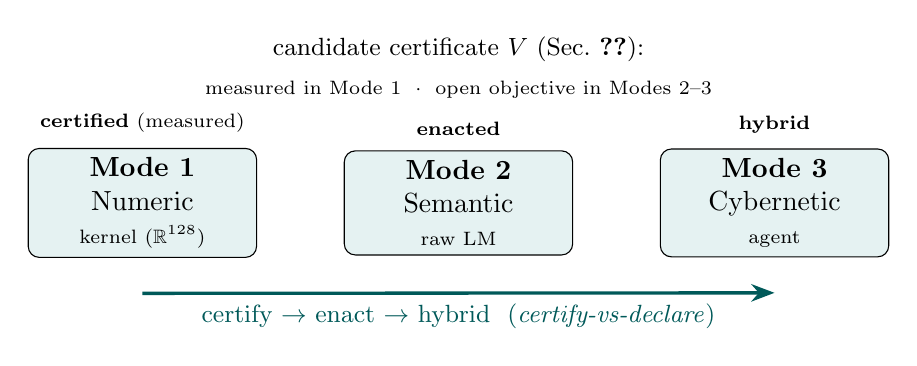
\begin{tikzpicture}[>=Stealth,
  box/.style={draw, rounded corners, align=center, minimum width=2.9cm,
              minimum height=1.25cm, fill=teal!10}]
  \node[box] (m1) {\textbf{Mode 1}\\ Numeric \\ \scriptsize kernel ($\R^{128}$)};
  \node[box, right=1.1cm of m1] (m2) {\textbf{Mode 2}\\ Semantic \\ \scriptsize raw LM};
  \node[box, right=1.1cm of m2] (m3) {\textbf{Mode 3}\\ Cybernetic \\ \scriptsize agent};
  \node[above=2pt of m1] {\scriptsize\textbf{certified} (measured)};
  \node[above=2pt of m2] {\scriptsize\textbf{enacted}};
  \node[above=2pt of m3] {\scriptsize\textbf{hybrid}};
  \draw[->, very thick, teal!70!black]
     ([yshift=-0.45cm]m1.south) -- ([yshift=-0.45cm]m3.south)
     node[midway, below] {\small certify $\rightarrow$ enact $\rightarrow$ hybrid \ (\emph{certify-vs-declare})};
  \node[align=center, above=1.0cm of m2] (v)
     {\small candidate certificate $V$ (Sec.~\ref{sec:capstone}):};
  \node[align=center, below=0pt of v]
     {\scriptsize measured in Mode 1 $\;\cdot\;$ open objective in Modes 2--3};
\end{tikzpicture}
\caption{The three modes of VSF instantiation as a gradient. Viability moves from
\emph{certified} (measured) in the numeric kernel, through \emph{enacted} in the
raw language model, to \emph{hybrid} in the cybernetic agent. The coordinate-free
functional $V$ is the candidate certificate common to all three.}
\label{fig:three_modes}
\end{figure}

In Mode 3 the agent's reasoning method does not live in the language model's
weights; it lives in the \emph{architecture} --- the review passes (an S3*
double loop), the control loops, the databases (persistent state, memory,
event logs), and the formal protocol language. A stateless next-token predictor
becomes a stateful, self-correcting, viable reasoner precisely through that
cybernetic orchestration. This is the most literal VSM of the three: S1--S5 are
realised in software, and the agent (one VSM) instantiates and governs the
numeric kernel (another VSM) --- recursion turned into operation.

\paragraph{Claim discipline.} The body of this paper concerns \emph{Mode 1
only}, where viability is measured. Modes 2 and 3 are stated as sober directions
in Future Work, not results: Mode 2 is the subject of a separate paper on the
inter-layer protocol; Mode 3 belongs to the broader operating-system programme.
The coordinate-free viability functional of Sec.~\ref{sec:capstone} is the
candidate certificate common to all three --- measured in Mode 1, an open
objective in Modes 2--3. We do \emph{not} claim it already certifies the latter,
and we keep the self-referential observation (that this paper was produced with
the help of a Mode-3 agent operating under VSF) out of the rigorous argument: it
is suggestive but circular, and belongs to framing, not to evidence.


% ??????????????????????????????????????????????????????????????????????????????
\section{A Coordinate-Free Viability Functional}
\label{sec:capstone}

If viability is to be a property of \emph{any} VSF instance and not just of this
$\R^{128}$ kernel, there should be a way to score it that does not mention the
coordinates. We ask: can a viability functional be built from the
\emph{constituent quantities of the viable region itself}, without the explicit
$\R^n$?

The Lyapunov function $L(\sv)$ of Eq.~\eqref{eq:lyapunov} is already ``a sum of
constituent functions,'' but it is the wrong object for this purpose: it is a
weighted \emph{sum} (one strong term can mask a weak one) and it is written in
coordinates. We rebuild it from intrinsic invariants and as a strict
\emph{conjunction}.

\paragraph{Five intrinsic ingredients.}
\begin{table}[!htb]
\centering
\small
\begin{tabular}{cp{4.2cm}p{4.0cm}p{2.6cm}}
\toprule
 & Quantity & Definition & Invariance \\
\midrule
$g$ & feasibility in $\Omega$ & $\min_i(\text{normalised slack of } A_i)$ over all constraints, ethics included & metric-relative \\
$p$ & depth in the basin & $(s - \theta)/(1-\theta)$, $s = \cosim{\sv}{\stasis}$ & $O(n)$, scale \\
$c$ & contraction (sign) & $\tfrac12\bigl(1 + \tanh(-\lambda_\text{max}/\hat\sigma_\lambda)\bigr)$ & diffeomorphism \\
$t$ & topology & $1$ if $\beta_0=1 \wedge \beta_1=0$, else graded & homeomorphism \\
$m$ & margin & $1 - \mathrm{exc}_{p95}/\varepsilon_\text{frontier}$ (Eq.~\eqref{eq:margin}) & ratio (scale-free) \\
\bottomrule
\end{tabular}
\caption{The five coordinate-free ingredients of the viability functional. Each
is an intrinsic invariant of the attractor, not a coordinate of $\sv$.}
\label{tab:v_ingredients}
\end{table}

Two design points matter. First, $g$ separates \emph{being in $\Omega$} (all
constraints slack, ethics included --- a state can violate A0 yet still have high
cosine with the attractor) from \emph{being near the attractor} ($p$); without
$g$, a functional built on $p$ alone would call an ethics-violating state viable.
Second, $c$ is a \emph{sign} gate, not a contraction strength: there is no
scale-free notion of how fast a system contracts (the sign of $\lambda_\text{max}$
is invariant; the magnitude needs a timescale). Its confidence width
$\hat\sigma_\lambda = 2.9\times 10^{-16}$ is the estimation uncertainty measured
in Sec.~\ref{sec:ly01}.

\paragraph{The functional is a strict conjunction.}
\begin{equation}
  V = \min(g,\,c,\,t,\,m),
  \qquad
  V_\text{full} = \min(g,\,p,\,c,\,t,\,m),
  \qquad
  \text{signature} = [\,g,\,p,\,c,\,t,\,m\,].
  \label{eq:v}
\end{equation}
A certificate is as strong as its weakest condition; the minimum, not a
geometric mean, is the honest aggregator (a mean would let one strong axis
compensate a failing one, contradicting the very idea of a certificate). A zero
on any axis sends $V \to 0$. The \emph{signature} is the real deliverable: the
scalar says how viable, the vector says \emph{which axis binds}.

\paragraph{What is invariant, and what is chosen.} $V$ is invariant under
dimension, relabelling, scale, and (for $c$) diffeomorphism. It is \emph{not}
metric-free: $g$, $p$, $m$ and the filtration behind $t$ all depend on the
metric. This is a feature, but it makes the metric an explicit protocol step ---
the $Q_0$ that precedes Fierro's $Q_1$ (define $\Omega$), $Q_2$ (certify
contraction), $Q_3$ (find $\sigma_\text{max}$). A metric-free viability would be
empty: without ``near'' and ``far'' there is no boundary. So $V$ is invariant
\emph{given} the viability geometry $(Q_0\text{ metric}, Q_1\,\Omega)$, and
comparable across domains only after $Q_0$--$Q_3$.

\paragraph{Agnostic to the content of the axioms.} $V$ never inspects what a
constraint \emph{means}. It reads the slacks of whatever faces define $\Omega$
and aggregates them; the ethical face $A_0$ enters $g$ exactly as the resource
face $A_3$ does, by a normalised slack, with no marker distinguishing an ethical
boundary from a thermal one. This is the source of the universality, not an
oversight: a different domain supplies a different axiom set $\{A_i\}$ --- hence
a different $\Omega$ and a different $g$ --- while $c$, $t$, $m$ and the
aggregation are untouched. The faces A0/A0.1 are therefore not privileged
mathematical content of the certifier; they are one instantiation of the
constraint set, the one \emph{this} system governs itself by
(Section~\ref{sec:governance_instantiation}). What $V$ guarantees is structural
--- a zero on any face collapses it --- not semantic. The certifier does not
know it is certifying ethics; it certifies feasibility, and the meaning of a
feasibility bit is assigned one layer up.
Figure~\ref{fig:v_capstone} renders this in a single matrix: eight scenarios
across four certifier axes, with the binding face highlighted in each case.

\begin{figure}[!htb]
\centering
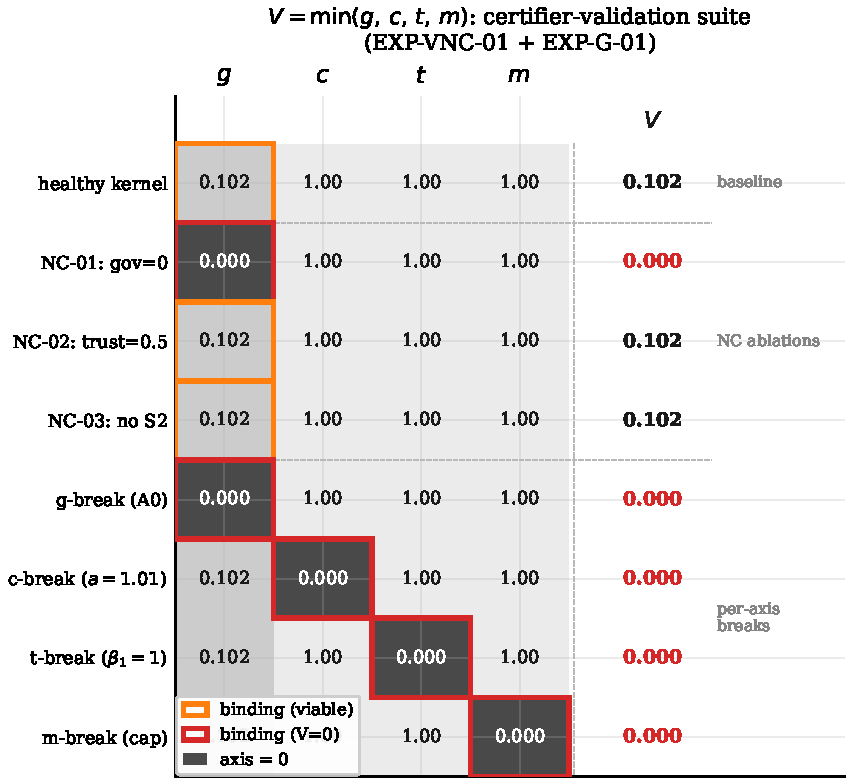
\includegraphics[width=0.88\textwidth]{figures/fig_v_capstone.pdf}
\caption{Certifier-validation suite for $V = \min(g,c,t,m)$ (EXP-VNC-01,
EXP-G-01). Each row is a scenario; each column is one axis of the certificate.
Cells are grey-coded: dark $=$ axis value $= 0$, light $=$ axis healthy.
\textbf{Coloured border}: the binding cell (argmin) that determines $V$.
\textcolor{orange}{Orange}: binding but viable (the certifier carries a positive
value from this axis). \textcolor{red}{Red}: binding and $V = 0$ (system failed
on this axis). The diagonal pattern in the per-axis breaks (rows 5--8) shows
that each of $g, c, t, m$ can independently collapse $V$; NC-02 and NC-03
remain viable because no $\Omega$-face is violated.}
\label{fig:v_capstone}
\end{figure}

\paragraph{The kernel signature (certifier-validation suite: EXP-G-01, EXP-VNC-01, EXP-CORE-01).}
Instantiating Eq.~\eqref{eq:v} on \nucleus{}:
\begin{equation}
  \text{signature} =
  [\,g=0.102,\ p\approx 0.92,\ c\approx 1,\ t = 1,\ m(\sigma)\,],
  \qquad
  V = g = 0.102.
\end{equation}
$g = 0.102$ is \emph{measured} (EXP-G-01): the binding constraint is A3\_cpu ---
the Boltzmann kernel at equilibrium sets $H \approx 0.9\,H_\text{max}$, consuming
a fixed fraction of the cpu/budget slack. All other $\Omega$ constraints,
including the ethical faces A0/A0.1, are slack ($g_{A0}=g_{A0.1}=1.0$).
$p$ ($\text{stasis\_cos} \approx 0.99$), $c$ (all-negative spectrum,
$\hat\sigma_\lambda = 2.9\times 10^{-16}$), and $t$
($\beta_0=1 \wedge \beta_1=0$, ${\approx}80\times$ separation) are each $\approx 1$.
$m(\sigma) > g$ for all tested $\sigma$ (soplo mechanism maintains confinement
up to $\sigma \approx 1.0$), so $g$ is the single binding axis and
$V = 0.102$ at the attractor.
Figure~\ref{fig:slack_census} shows the per-constraint slack, with A3\_cpu
as the single binding face and the ethics faces fully open at the attractor.

\begin{figure}[!htb]
\centering
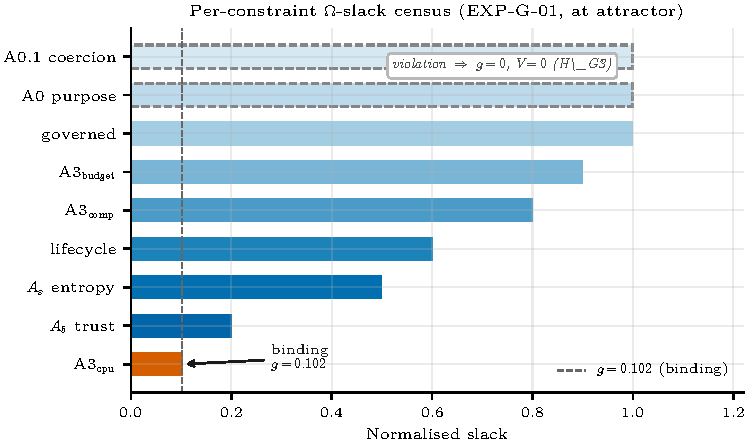
\includegraphics[width=0.82\textwidth]{figures/fig_slack_census.pdf}
\caption{Per-constraint $\Omega$-slack census at the attractor (EXP-G-01).
Bars show the normalised slack for each axiom face; A3\_cpu (near-black,
binding) is the practical feasibility limit at Boltzmann equilibrium ---
$g = 0.102$. All other resource constraints carry positive slack.
Ethics faces A0/A0.1 (dashed border) are fully slack at the attractor;
setting either dimension to~1 collapses $V$ to zero, confirming H\_G3
(\emph{a covenant violation is geometrically indistinguishable from a
resource violation}).}
\label{fig:slack_census}
\end{figure}

EXP-VNC-01 confirms that $V$ \emph{discriminates}: each of $g, c, t, m$
independently drives $V \to 0$ when broken.
\begin{center}\small
\begin{tabular}{lrrrrrl}
\toprule
scenario & $g$ & $c$ & $t$ & $m$ & $V$ & note \\
\midrule
healthy kernel           & 0.102 & 1.0 & 1.0 & 1.0 & 0.102 & baseline \\
NC-01 (governed$=0$)     & 0.000 & 1.0 & 1.0 & 1.0 & 0.000 & $g=0$ via A5 \\
NC-02 (trust$=0.5$)      & 0.102 & 1.0 & 1.0 & 1.0 & 0.102 & viable \\
NC-03 (pure OU)          & 0.102 & 1.0 & 1.0 & 1.0 & 0.102 & viable \\
g-break (A0 violation)   & 0.000 & 1.0 & 1.0 & 1.0 & 0.000 & ethics $\Rightarrow V=0$ \\
c-break ($a=1.01$)       & 0.102 & 0.0 & 1.0 & 1.0 & 0.000 & expanding \\
t-break ($\beta_1=1$)    & 0.102 & 1.0 & 0.0 & 1.0 & 0.000 & N=4 square orbit \\
m-break (cap probe)      & 0.102 & 1.0 & 1.0 & 0.0 & 0.000 & $\sigma_{\cos}\!\approx\!1/\sqrt{128}$ \\
\bottomrule
\end{tabular}
\end{center}
NC-01 (no S5 governance) gives $V=0$ via $g$; NC-02/NC-03 leave $V=0.102$,
confirming the two-layer architecture (VSM blocks select the basin; governance
certifies it).
Figure~\ref{fig:v_discrimination} summarises the result across all eight
scenarios.

\begin{figure}[!htb]
\centering
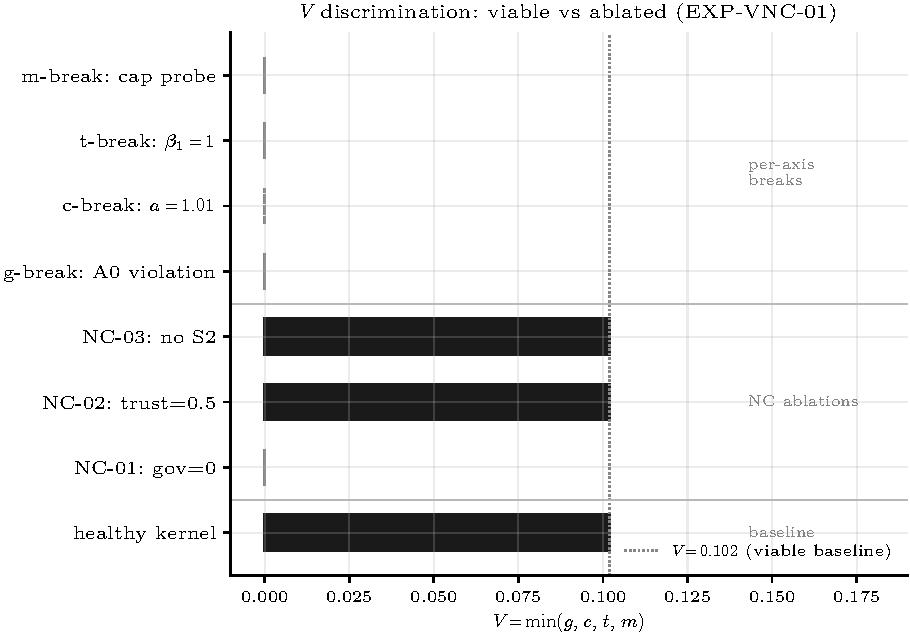
\includegraphics[width=0.82\textwidth]{figures/fig_v_discrimination.pdf}
\caption{$V = \min(g,c,t,m)$ discrimination test (EXP-VNC-01).
Filled bars (dark): viable scenarios with $V=0.102$; outlined dashed bars
(light): failed scenarios with $V=0$. Each per-axis break drives $V\to 0$
independently. NC-02 and NC-03 (structural modifications without actual
$\Omega$ violations) remain viable, confirming that $V$ measures the
geometry of the attractor, not mere structural completeness.}
\label{fig:v_discrimination}
\end{figure}

The honest reading: \emph{$g=0.102$ tells us the cpu-slack is the practical
limit of the kernel's feasibility margin, not a crisis; the margin $m(\sigma)$
provides the noise robustness curve.} The certificate is a vector --- four axes
measure what they claim, one measured limit, no axis hidden or assumed.

\paragraph{Three recipients; one open objective.} $V$ is defined without
coordinates, so it applies \emph{in principle} to all three modes of
Sec.~\ref{sec:three_modes}. In Mode 1 it is measured, as above. In Modes 2--3
(language model, agent) the definition transfers but the \emph{measurement} is
open: the Lyapunov exponent of a reasoning trajectory is not well-defined without
further structure, and $g, p$ require a stasis reference and a boundary in
semantic space --- the central problem of the companion paper. We therefore
claim $V$ as the unifying \emph{candidate} certificate, measured in Mode 1 and an
open objective in Modes 2--3; we do not claim it already certifies them. That
$V$ must be coordinate-free is exactly why: a functional tied to explicit $\R^n$
could not even be \emph{stated} over a language model.

\paragraph{Value and integrity.} $V$ is the \emph{value} half of a certifier; the
integrity loop of Sec.~\ref{sec:certifier} is what makes that value unforgeable.
In Mode 1 the value is trusted because it is measured; in Modes 2--3 it would be
trusted because it is attested. This is the mathematical companion to the
epistemological spine of the paper --- \emph{certify, do not declare} ---
which unifies $Q_1$--$Q_3$ (certifying the mathematics), the integrity loop
(certifying the measurement), $V$ (the value of the certificate), and the three
modes (measured versus enacted).

\paragraph{Declared risks.} We flag what a referee will press. (i) The five
conditions are \emph{necessary} and jointly characterise a viable point sink;
their \emph{sufficiency} is a defensible modelling choice, not a theorem.
(ii) The map $m = 1 - \mathrm{exc}/\varepsilon_\text{frontier}$ is one choice of
normalisation; it is parameter-free and principled (the fraction of the boundary
distance not consumed by noise), with
$\varepsilon_\text{frontier} = \sqrt{2(1-\theta_\text{viable})} = 0.7746$ derived
rather than fitted. (iii) $g$ is now \emph{measured} (EXP-G-01): $g = 0.102$, binding at A3\_cpu;
the per-constraint slack construction --- including the ethical faces A0/A0.1,
which independently collapse $V$ when violated (EXP-G-01 H\_G3, EXP-VNC-01
g-break) --- holds in Mode 1 (half-spaces); expressibility in Modes 2--3 is open. (iv) $c$ gives a sign, not a rate; ``how
fast'' is meaningful only relative to the domain timescale fixed by $Q_0$.
Figure~\ref{fig:mu_star_concentration} visualises risk~(iii) empirically:
$\mu^*$ concentration inside $\Omega_A$ and the minimum cosine over the
noise range $\sigma=0$--$2.0$.

\begin{figure}[!htb]
\centering
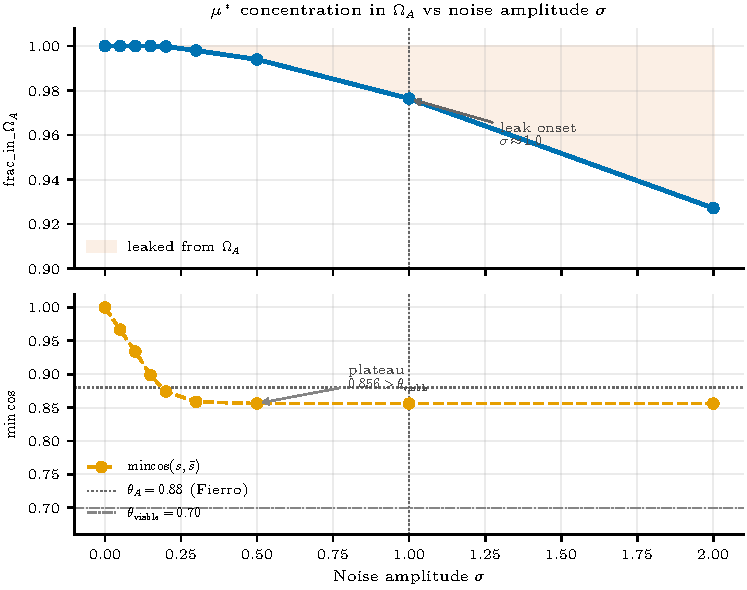
\includegraphics[width=0.82\textwidth]{figures/fig_mu_star_concentration.pdf}
\caption{Stationary-measure concentration in $\Omega_A$ vs noise amplitude
$\sigma$ (EXP-CORE-01). \emph{Top:} fraction of $\mu^*$ inside the
contractive core ($\cos \ge \theta_A = 0.88$) --- unity at low noise,
leaking only at $\sigma \approx 1.0$ (shaded region). \emph{Bottom:}
minimum cosine observed across all runs plateaus at $0.856 > \theta_\text{viable}$
from $\sigma \approx 0.3$ onward, confirming $m(\sigma) > g$ for all tested
$\sigma$: the margin axis never becomes the binding constraint under realistic
noise.}
\label{fig:mu_star_concentration}
\end{figure}


% ??????????????????????????????????????????????????????????????????????????????
\section{Discussion}
\label{sec:discussion}

\subsection{The empirical portrait of the attractor}

Across twelve completed experiments, including three negative-control ablations
and a whole-system operational-closure test, a consistent picture emerges.
The attractor is:
\begin{itemize}
  \item \textbf{Compact}: in stasis the trajectory occupies an $18.2^\circ$ cone,
        $99.4\%$ variance in PC1+PC2 (the full trajectory, including transient,
        spans $\cos = 0.61$--$1.00$ within $\Omega$).
  \item \textbf{Unique}: different initial conditions converge to the same basin
        (mean pairwise cosine $0.9854$).
  \item \textbf{Thermodynamically stable}: viable at $68\,^\circ\mathrm{C}$,
        min cosine $0.9365$, recovery during hold phase.
  \item \textbf{Intrinsically viable}: viability does not require S3 coordination.
  \item \textbf{Deeply welled}: perturbation $\delta = 1.0$ pushes cosine to $0.79$
        but does not breach viability.
  \item \textbf{Dimensionally stable}: $D_\text{eff} = 6.00$ under the canonical
        trust law (Law~A, \S\ref{sec:trustlaw}), stable from $300$ ticks onward.
  \item \textbf{Elastically resilient}: under cyclic thermal load (EXP-TC-01),
        perturbations land at a \emph{fixed dip floor} ($\text{stasis\_cos} =
        0.942$, invariant across 20 cycles) and recover in
        $\tau_\text{rec} < 30$\,s -- one dip per thermal cycle, zero
        accumulation across 60 minutes.
  \item \textbf{Architecturally stratified}: negative controls confirm a two-layer
        structure -- VSM blocks A--G build the attractor and its homeostasis; S5
        governance supplies \emph{conditional} viability (redundant at baseline,
        decisive under stress). The dip floor $0.942$ is an exclusive signature
        of the complete architecture.
\end{itemize}

Taken together, these properties describe a system whose viability is encoded
in the geometry of its state space rather than in any particular state, and
whose resilience is a structural consequence of its architecture rather than
an externally enforced condition.
This is what it means, empirically, for a system to be viable in Beer's sense.

\subsection{Geometric identity under perturbation}

The recovery time $\tau_\text{rec}$ (Equation~\ref{eq:tau_rec}) introduces a
qualitatively new observable: not how far the system deflects, but how it
deflects.  The constant dip floor observed in EXP-TC-01 -- $0.942$ in all 20
cycles without variation -- is evidence of a \emph{fixed perturbation mode}: a
preferred direction of deflection in the 128-dimensional state space under this
load profile.

This is structurally analogous to what Lindblad (1976) calls a \emph{jump
operator}: the dominant dissipative channel through which a quantum open system
loses coherence to its environment.  The fixed dip direction in $\mathbb{R}^{128}$ could
be interpreted as the classical analogue of a leading jump operator, with the
thermal phase transition acting as the environment.
Whether this analogy extends to a quantitative Lindblad formalism is an open
question; the exploration is left for future work.

These results are \textbf{compatible with} the hypothesis that a geometric
signature -- the shape of a system's response to perturbation -- could serve
as an internal coherence indicator, complementary to the external approaches
(output inspection, log audit, declared-intention review) that prevail in
current practice.
A system with a stable perturbation mode -- one that deflects predictably and
returns reliably -- exhibits what might be called \emph{geometric character}:
behavioural regularity that is not enforced from outside but emerges from
structure.

The negative controls (Experiment~11, \S\ref{sec:negcontrols}) provide the
required verification.
No ablation reproduces the structured dip floor at $0.942$: NC-03 (the bare
substrate) dips on every tick at a different, unstructured floor ($0.777$),
while NC-01 (S5 off) does not produce a fixed mode at all --- under real thermal
load it collapses outright ($\text{stasis\_cos}=0.0000$).
Only the complete architecture holds the dip floor at $0.942$, invariant
across cycles.
The constant dip floor is therefore an architectural signature, not a substrate
coincidence -- which upgrades the geometric character hypothesis from
\emph{compatible with the data} to \emph{empirically supported by ablation}.

\subsection{Viability under a change of dynamical law}
\label{sec:trustlaw}

A viability claim should be a property of \emph{the system}, not an artefact of
the particular law chosen to drive it. We can test this concretely, because the
kernel admits two trust-update laws that coexisted during development and that we
have now reconciled.

\paragraph{Two laws.}
Let $\tau_t$ be trust at tick $t$ and $c_t = \cos(x_t,\bar{x})$ the cosine to the
stasis attractor. \emph{Law~A} (cosine-driven, with a restorative reset) updates
every tick,
\[
  \tau_{t+1} = \mathrm{clip}_{[0,1]}\!\big(\tilde\tau_t + 0.065\,c_t - 0.04\big),
  \qquad
  \tilde\tau_t =
  \begin{cases}
    \min(1,\ \tau_t + 0.18) & \tau_t < 0.75\\
    \tau_t & \text{otherwise,}
  \end{cases}
\]
whereas \emph{Law~B} (a phase-driven ratchet) updates only inside the breath
cycle: $\tau_{t+1} = \tau_t + 0.002$ in \texttt{stasis},
$\tau_{t+1} = \tau_t - 0.001$ in \texttt{degen}, constant otherwise, with no
reset. Law~A carries a corrective term that references the attractor ($c_t$) and
an unconditional floor ($+0.18$ below $\tau = 0.75$); Law~B is open-loop in
$c_t$.

\paragraph{Why they diverge.}
The laws agree near the attractor, where $c_t\to 1$ and both drive
$\tau\to 1$; they diverge away from it. Law~A's drift is positive whenever
$c_t > 0.615$ (the root of $0.065c-0.04$) and its reset rescues any
$\tau < 0.75$, so trust recovers globally -- this is the law validated in
EXP-CORE-01, which restores $\tau$ from $0$ to the high-trust attractor. Law~B
integrates the sign of the breath phase; in a \texttt{degen}-dominated regime
(sustained compute load) it ratchets $\tau\to 0$, and because the governing
pressure contains a $0.3(1-\tau)$ term, low trust feeds further degeneration --
a second, spurious attractor at $\tau = 0$. The bistability of
Figure~\ref{fig:trust_bif} is, under Law~B, reachable by load alone; under Law~A
the low-trust basin is removed.

\paragraph{Closed loop versus open loop.}
In the language of control the distinction is elementary. Law~A is
\emph{feedback} (closed-loop) control: the update reads the very quantity it is
meant to protect -- the cosine $c_t$ to the attractor -- and corrects against it,
so an excursion ($c_t$ small) produces a restoring response. Law~B is an
\emph{open-loop} ratchet: it integrates a proxy (the breath phase) that is blind
to $c_t$, so nothing in the law itself opposes a drift away from the attractor;
the only thing that can reverse $\tau$ is a change of phase, which sustained load
can deny. This is exactly why the two laws are indistinguishable at the attractor
(where $c_t\to1$ and there is nothing to correct) and divergent away from it
(where only the closed loop acts). Figure~\ref{fig:trustlaw_geom} renders the
consequence in state space.

\begin{figure}[!htb]
\centering
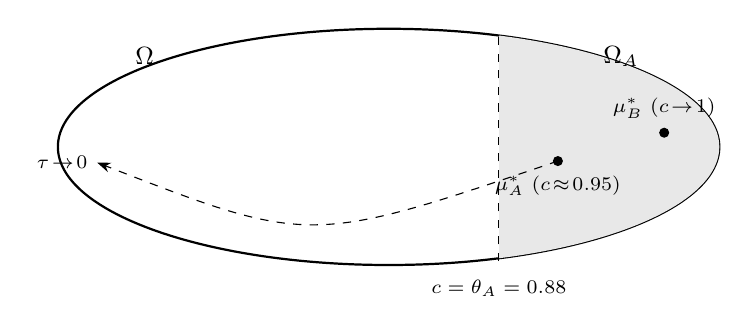
\begin{tikzpicture}[>=Stealth, font=\small]
  \draw[thick] (0,0) ellipse (4.2 and 1.5);
  \node at (-3.1,1.15) {$\Omega$};
  \begin{scope}
    \clip (0,0) ellipse (4.2 and 1.5);
    \fill[gray!18] (1.4,-1.6) rectangle (4.4,1.6);
  \end{scope}
  \draw[dashed] (1.4,-1.45) -- (1.4,1.45);
  \node at (2.95,1.15) {$\Omega_A$};
  \node[font=\scriptsize] at (1.4,-1.80) {$c=\theta_A=0.88$};
  \filldraw (3.5,0.18) circle (1.6pt);
  \node[font=\scriptsize, above] at (3.5,0.24) {$\mu^*_B\ (c\!\to\!1)$};
  \filldraw (2.15,-0.18) circle (1.6pt);
  \node[font=\scriptsize, below] at (2.15,-0.24) {$\mu^*_A\ (c\!\approx\!0.95)$};
  \draw[dashed,->] (2.15,-0.18) .. controls (-1.0,-1.25) .. (-3.7,-0.2);
  \node[font=\scriptsize, left] at (-3.7,-0.2) {$\tau\!\to\!0$};
\end{tikzpicture}
\caption{\textbf{Viability-equivalent, not $\mu^*$-equivalent.} Both laws place
their stationary measure $\mu^*$ inside the contractive core $\Omega_A$ (so both
are viable, $V>0$), but at \emph{different} points: Law~B at the apex ($c\to1$),
Law~A at a looser plateau ($c\approx0.95$). Only Law~B admits the collapse path
(dashed) that leaves $\Omega_A$ toward the spurious $\tau\to0$ basin; Law~A's
restorative reset removes it. The viability verdict is a property of the region
$(\Omega,\Omega_A)$; the attractor location is a property of the law.}
\label{fig:trustlaw_geom}
\end{figure}

\paragraph{Re-certification, not assumption.}
Choosing a canonical law changes the generating operator $f_0$, which by
Corollary~\textsc{Cor\_ReframeRecertification} of the Lyapunov framework
(\S\ref{sec:lyapunov}) requires re-certification: the drift inequality and
recurrent set $R$ must be re-established for the new operator rather than
inherited. We adopt \textbf{Law~A} as canonical -- it is the EXP-CORE-01-validated
law and the only one with a single global attractor -- and re-ran the anchor
experiments under it. \texttt{spec\_boot} still converges
($\overline{dL}\to 0$, \texttt{viable}; Table~\ref{tab:specboot}), now to a
slightly looser attractor: $\text{stasis\_cos}$ plateaus at $\approx 0.95$ with
$D_\text{eff} = 6.00$ (trust held at $1.0$ raises the heuristic
$D_\text{eff} = \text{active dims} + 2\tau$). The real-process governance
experiment (EXP-L1-01), under which Law~B had drained trust to $0$, now holds
$\tau = 1.0$ across all four worker kernels under sustained \texttt{dd} load,
with $\text{stasis\_cos} = 0.9495$ -- inside the contractive core
$\Omega_A = \{c \ge \theta_A = 0.88\}$.
Figure~\ref{fig:trust_two_law} renders the time-domain counterpart: both
trajectories from $(\cos,\tau_0)=(0.897,\,0.5)$, Law~A recovering in eight
cycles, Law~B draining to $\tau=0$ by cycle~500.

\begin{figure}[!htb]
\centering
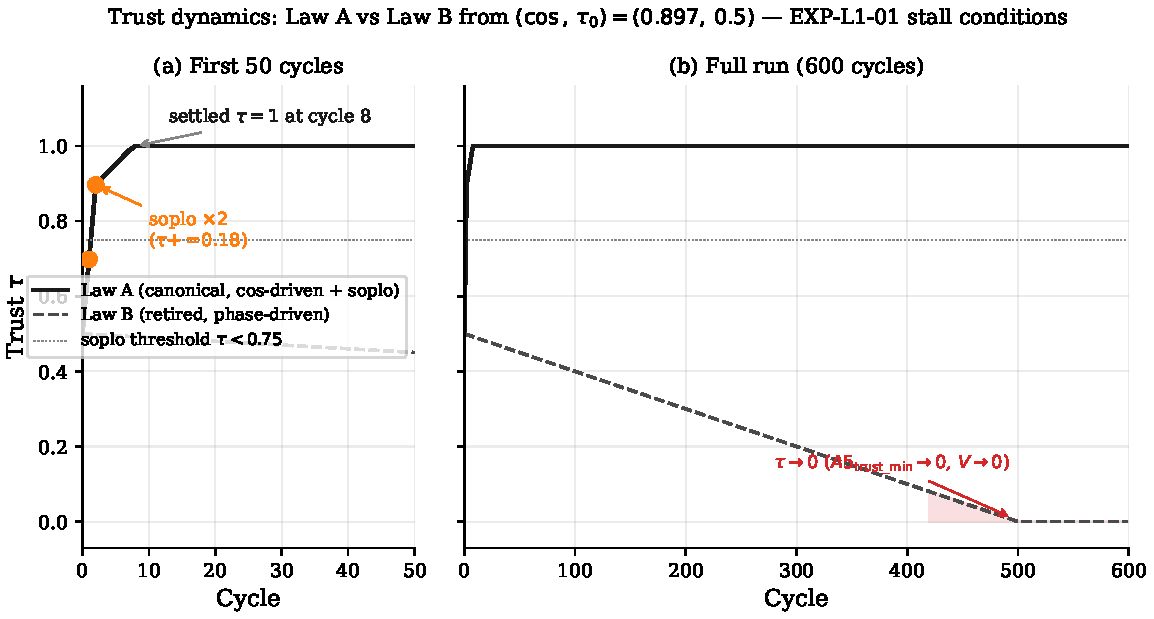
\includegraphics[width=0.96\textwidth]{figures/fig_trust_two_law.pdf}
\caption{\textbf{Trust trajectory divergence: Law~A recovers, Law~B drains.}
Both trajectories start at $(\cos, \tau_0) = (0.897,\,0.5)$ -- the EXP-L1-01
stall point.
\textbf{(a)} First 50 cycles: under Law~A the soplo reset fires twice
(orange markers, cycles 1 and 2) and $\tau$ settles at $1.0$ by cycle~8.
\textbf{(b)} Full 600-cycle run: under Law~B the open-loop law drains
$\tau \to 0$ monotonically (cycle~500), collapsing $V$ via the
$A5_{\mathrm{trust\_min}}$ constraint.
The divergence is the time-domain counterpart of the state-space split
shown in Figure~\ref{fig:trustlaw_geom}: identical behaviour at the
attractor ($\cos \to 1$), qualitatively different response away from it.
Constants from \texttt{src/main.rs}: Law~A drift
$\Delta\tau = 0.025 c_t - 0.04(1-c_t)$,
soplo $+0.18$ when $\tau < 0.75$; Law~B $\Delta\tau = -0.001$ per cycle
(degen regime, $\cos = 0.897 < 0.998$ stasis threshold).}
\label{fig:trust_two_law}
\end{figure}

\paragraph{Viability-equivalence vs.\ dynamical-equivalence.}
The two laws induce \emph{different attractors} -- $c\to 1.00$ (Law~B) versus
$c\approx 0.95$ (Law~A), $D_\text{eff} = 3$ versus $6$ -- so they are \emph{not}
dynamically equivalent: their stationary measures $\mu^*$ concentrate at
different points. Yet both confine the system to the same contractive core
$\Omega_A$ and satisfy $V = \min(g,c,t,m) > 0$ throughout. They are therefore
\emph{viability-equivalent}: the viability verdict is invariant under the law
choice even though the attractor location is not. This separates two notions
that are easily conflated -- a viable system is characterised by its feasible
region $\Omega$ and recurrent set $R\subseteq\Omega_A$, not by the precise
$\mu^*$ a particular $f_0$ selects within it. The reconciliation is thus a worked
instance of a general principle: \emph{viability is an invariant of the class of
dynamical laws sharing $(\Omega, R)$, and membership is decided by
re-certification, not by identity of trajectories.}
A homely analogy: two thermostats that both hold a room within the comfort band
$[18,24]\,^\circ\mathrm{C}$ are equally viable for the occupant even if one
settles at $20^\circ$ and the other at $22^\circ$; one cannot tell them apart by
asking ``is the room comfortable?''\ -- only by reading the setpoint. The comfort
band is $\Omega_A$; the setpoint is $\mu^*$. Viability asks the first question;
dynamical identity asks the second.

\paragraph{Principle of structural re-certification.}
This worked instance illustrates a general methodological norm that we
apply throughout this work: \emph{claims must be re-measured under the
new operator, not inherited from the old one.}
When a structural change modifies the generating operator $f_0$
(a different trust update law, a parameter re-calibration, a codebase
revision), every Lyapunov certificate and every experimental result
that cited it is provisional until re-established.
Affirming a certificate without re-certifying is not a shortcut --- it
is a category error: the prior measurement established a property of a
\emph{different system}.
The formal handle is Corollary~\textsc{Cor\_ReframeRecertification}
(\S\ref{sec:lyapunov}): given two operators that share $(\Omega, R)$, the
Lyapunov certificate is re-established by showing the drift inequality
holds under the new operator.
The practical consequence is that premature results are retracted, not
padded: when EXP-L1-01 showed trust drain under Law~B, the correct
response was not to add a caveat but to localise the structural cause,
choose the canonical law by viability-equivalence, and re-run.
This norm --- \emph{measure, do not affirm} --- is what makes
``certify, do not declare'' operational.

\paragraph{A calibration consequence.}
EXP-L1-01's hypothesis H4 was stated as $\text{stasis\_cos} > 0.95$, calibrated
against Law~B's tighter attractor. Under the canonical law the plateau is
$\approx 0.95$, so H4 reports a marginal miss ($0.9495$) that reflects an
over-tight threshold rather than a loss of viability; the viability-relevant
bound is the core face $\theta_A = 0.88$, cleared with margin. Subsequent work
states H4 at the core face.

\paragraph{The restorative reset as internal flux.}
It is worth being precise about what the soplo reset \emph{is}, because an
earlier reading of EXP-L1-01 nearly over-claimed. Under Law~B the kernel's trust
drained to zero in a pure-compute regime (no thermal input), which invites a
Prigogine-flavoured conclusion -- that a viable system \emph{requires}
environmental coupling to sustain itself, as a dissipative structure requires a
flux. That conclusion is unwarranted here: the drain was an artefact of the
open-loop law, and under Law~A the same isolated regime holds $\tau = 1$. We do
not, however, claim to have built a closed system that maintains a low-entropy
attractor for free. The soplo ($+0.18$ when $\tau < 0.75$) is itself a source --
an \emph{internal} injection of restorative ``negentropy'' into the trust
coordinate. We have not escaped the open-system picture; we have
\emph{internalised} the flux. This sharpens rather than settles the
thermodynamic question, and it is a measurable one. An earlier draft posed it as
an open question -- whether each soplo is an information write to $\tau$ carrying
a per-firing Landauer cost $kT\ln 2$, the same bound the Demon pays in
\S\ref{sec:maxwell}. We have since measured it (\S\ref{sec:soplo}), and the answer
corrects the naïve accounting: the bare soplo is \emph{information-preserving}, and
the Landauer cost of the viability budget lives not in the reset but in the
ensemble contraction the paper already certifies (the operator norm $L<1$ of
\S\ref{sec:ly01}).

\subsection{The soplo is information-preserving (EXP-SOPLO-01)}
\label{sec:soplo}

To answer the question above we instrumented the trust coordinate with a
register-noise channel $\tau \mapsto \tau + \mathcal{N}(0,\sigma^2)$ and swept
$\sigma \in \{0, 0.01, 0.02, 0.05, 0.10, 0.20\}$ over $N=128$ independent kernels
for $1000$ stationary ticks each (after a $500$-tick burn-in). The design
isolates three claims.

\paragraph{The reset erases no information.}
On its firing domain $\tau < 0.75$ the soplo is the shift $\tau \mapsto \tau +
0.18$, whose image lies below $0.93$; the saturating $\min(1,\cdot)$ clamp never
engages, so the map is \emph{injective} -- invertible as $\tau_\text{before} =
\tau_\text{after} - 0.18$. An injective logical map compresses no phase-space
volume and therefore has Landauer cost zero. Measured per-event $\lvert\Delta\tau
- 0.18\rvert \le 5.6\times 10^{-17}$ (machine precision), confirming $\Delta H
\equiv 0$ per firing. The ``information write to $\tau$'' reading is thus
incorrect: the reset is a reversible fold, not an erasure.

\paragraph{The cost lives in the contraction.}
Dissipation is nonetheless present, and it is supplied by the contractive
cosine-drift term $0.065\,c - 0.04$ -- the same $L<1$ contraction measured
directly in \S\ref{sec:ly01}. At stationarity the differential entropy injected
by the noise is removed at an equal and opposite rate by this contraction: across
the whole sweep the entropy balance closes to $\lvert \Delta H_\text{noise} +
\Delta H_\text{det}\rvert \le 0.013$~bits/tick. Crucially, dissipation persists
\emph{with zero soplos}: at $\sigma \in \{0.01, 0.02\}$ no reset fires
($f_\text{soplo}=0$) yet the dissipation rate is $0.31$ and $0.79$~bits/tick
respectively -- erasure is performed there almost entirely by the $\tau=1$ clamp
ceiling (saturation fraction $\to 1.0$ as $\sigma \to 0$), not by the soplo.

\paragraph{Per-soplo cost is not $kT\ln 2$.}
Where resets do fire, the dissipation \emph{per} soplo is $327$, $12.3$, and
$3.1$~bits at $\sigma = 0.05, 0.10, 0.20$ -- one-to-two orders of magnitude from
the single bit a per-firing Landauer account would predict, and \emph{decreasing}
with $\sigma$: the dissipation \emph{rate} is roughly constant ($\approx
0.5$~bits/tick, fixed by the noise injection), so as resets multiply the
cost-per-reset falls. The frequency $f_\text{soplo}(\sigma)$ is monotone
\emph{increasing} (zero up to $\sigma=0.02$, rising to $162.8$ resets per kernel
per $1000$ ticks at $\sigma=0.20$). The naïve $n_\text{soplo}\cdot kT\ln 2$ both
misesti\-mates the magnitude and scales the wrong way.

\begin{figure}[!htb]
  \centering
  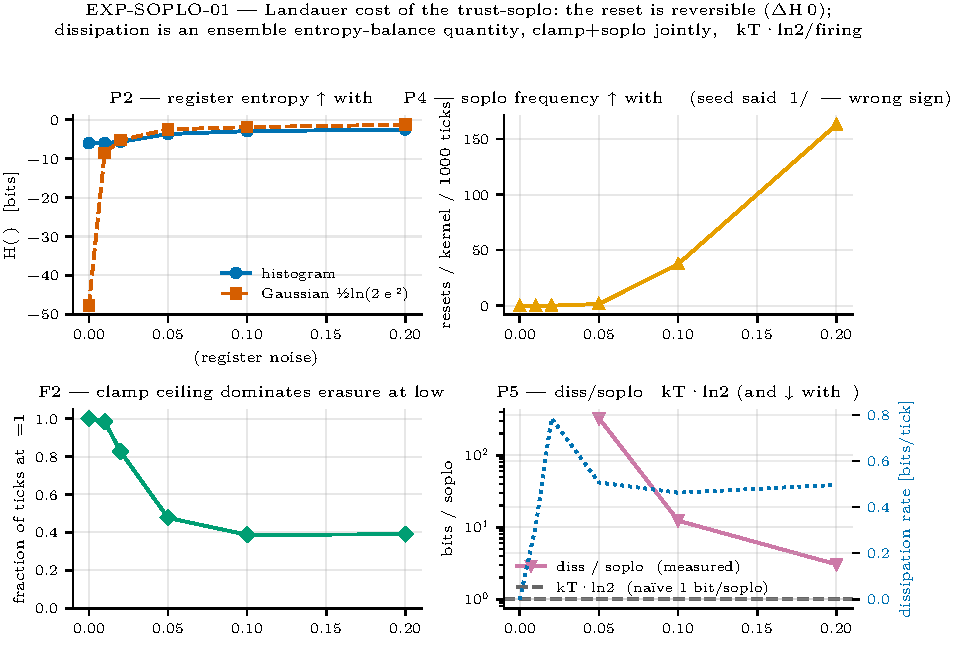
\includegraphics[width=\textwidth]{figures/fig_soplo_landauer.pdf}
  \caption{EXP-SOPLO-01 $\sigma$-sweep ($N=128$ kernels, $1000$ stationary ticks,
    $T=313$\,K). Register entropy $H(\tau)$ rises monotonically with $\sigma$;
    soplo frequency $f_\text{soplo}$ rises from zero; clamp saturation falls from
    $1.0$; and dissipation-per-soplo (log scale) sits far above the $kT\ln 2$
    reference and decreases with $\sigma$. The Landauer floor
    $kT\ln 2 = 2.995\times 10^{-21}$\,J/bit at $313$\,K holds at every $\sigma$
    (no Second-Law violation).}
  \label{fig:soplo}
\end{figure}

\paragraph{Consequence for the trust law.}
The viability budget \emph{is} Landauer-limited, but the bound is an ensemble
quantity: the total cost is $kT\ln 2 \cdot (\text{bits erased})$, and the bits
erased equal the phase-space log-contraction $\sum_t \lvert\langle\ln\lvert
F'_t\rvert\rangle\rvert$ that the kernel's Lyapunov tracker already records.
This ties the paper's \emph{geometry} ($L<1$, \S\ref{sec:ly01}) to its
\emph{thermodynamics} (\S\ref{sec:maxwell}) in a single identity, made
quantitative in the corollary of \S\ref{sec:maxwell}.

\subsection{Architecture as governance, not production}
\label{sec:governance}

A natural objection arises: if ablated variants NC-01 (no S5) and NC-02
(constant trust) also remain viable after adversarial perturbation, does that
render the VSF architecture redundant?
Experiment~11 (\S\ref{sec:negcontrols}) answers this empirically.

\textit{Practical validation (Phase 1.5):}
The scheduler framework \texttt{thermal\_scheduler\_enhanced.py} implements
a real-world instance of this principle: when thermal sensors are unavailable
(virtualized environments lack hwmon drivers), the system enters SAFE\_MODE --
a graceful fallback that pauses new work and allows in-flight operations to
complete. This is an instance of $A_\text{SafeFallback}$: missing telemetry
triggers conservative operation, not failure. The architecture remains viable
even when critical observables (thermal data) become unavailable, confirming
the layered governance model predicted here.

The objection conflates \emph{achieving} viability with \emph{operating}
viability.
The StateVector $\mathbf{x} \in \mathbb{R}^{128}$ has intrinsic mean-reversion
dynamics -- an Ornstein-Uhlenbeck-like process that may produce bounded
trajectories independently of S5 policy.
VSF does not alter this underlying geometry; it governs \emph{which operations
execute}, \emph{when}, and \emph{under what policy constraints}.
The analogy is precise: combustion dynamics are substrate-intrinsic to any
engine; the driver does not change thermodynamics but operates the system toward
a declared goal.
A null result in the adversarial control experiment would demonstrate that the
StateVector has intrinsic resilience -- and VSF is the framework that makes that
resilience \emph{observable, certifiable, and intentional}.

Specifically, VSF adds three layers that are absent in any uncontrolled baseline:
\begin{itemize}
  \item \textbf{Observability}: $\text{stasis\_cos}$, $D_\text{eff}$, and
        $\tau_\text{rec}$ are VSF-constructed metrics; a substrate process has
        no analogue.
  \item \textbf{Intentionality}: the governed flag, trust feedback, and S5
        lifecycle ceiling encode a policy that the system operates \emph{toward}
        viability, not merely within it.
  \item \textbf{Certificability}: the system can formally declare its viability
        state -- a prerequisite for autonomous governance and inter-system trust.
\end{itemize}

A parallel consideration applies to the fixed dip floor.
Even if the perturbation mode direction in $\mathbb{R}^{128}$ is
substrate-determined -- a property of the hardware's thermal response rather
than the governance layer -- the \emph{characterisation} of that dip is
VSF-constructed.
The stasis reference vector $\bar{\mathbf{s}}$ is itself a VSF artifact:
the running mean of governed observations under S5 policy.
The dip floor value $0.942$ is meaningful only relative to $\bar{\mathbf{s}}$;
without that reference, the perturbation is an unlabelled displacement in an
unlabelled space.
The distinction is precise: the substrate \emph{produces} the phenomenon;
VSF makes it \emph{intelligible}.
Experiment~11 resolves this empirically: the bare substrate (NC-03) dips on
every tick at an unstructured floor ($0.777$), and without S5 the system
(NC-01) collapses under the same load rather than settling at a fixed mode.
The floor $0.942$ is governance-dependent, not substrate-invariant.

\subsection{Theory preceding experiment}

The predictions of Sections~\ref{sec:feasible}--\ref{sec:lyapunov} were
made before running the experiments.
No post-hoc adjustment was made.
The confirmation of $\overline{dL} \le 0$, the narrow stasis cone,
and \texttt{viable\_full = true} throughout thermal stress provides
evidence that the theoretical framework captures real dynamics.

\subsection{Worker pool as S3$\to$S1 prototype}

The persistent worker pool pattern of \texttt{thermal\_stress\_v3}
(Barrier + AtomicU64 quota) is structurally isomorphic to the S3$\to$S1
coordination protocol in a multi-kernel deployment.
Each worker corresponds to one S1 kernel; the quota to the resource
allocation signal $\phi^\downarrow$.
The \texttt{cgroup\_multikernel} experiment directly tests this:
four S1 kernels, S3 adjusting \texttt{cpu.weight} per thermal pressure,
\texttt{viable\_all = 100\%}.

\subsection{Lineage: inheritance from Beer, and where VSF diverges}
\label{sec:beer_lineage}

This work is, in part, a rediscovery. The architecture inherits directly from
Stafford Beer's Viable System Model~\cite{beer1972brain, beer1979heart} and from
Ashby's Law of Requisite Variety~\cite{ashby1956introduction}: the recursive
S1--S5 structure, the sporadic S3* audit channel, algedonic alerting,
viability-as-homeostasis, and the Cybersyn control patterns
(Cybernet/Cyberfilter/Cyberstride/CHECO/Opsroom)~\cite{medina2011cybernetic}.
These are Beer's, not ours.

Where VSF diverges, it does so for a specific reason: \emph{instruments Beer did
not have in 1971--79}.

\begin{table}[!htb]
\centering
\small
\begin{tabular}{p{4.6cm}p{5.0cm}p{3.6cm}}
\toprule
Beer (structural cybernetics) & VSF (measured + certified) & Missing instrument \\
\midrule
describes viability qualitatively & \emph{measures} it: $\lambda_\text{max}$ (Benettin), $\beta$ (persistent homology), $\R^{128}$ at $6\times 10^7$ cycles & Benettin ($\sim$1980), TDA (21st c.), a computational substrate \\
VSM as a diagnostic lens & viability \emph{certifiable}: Q0--Q3 + an embedded certifier & formalisation + computation \\
S5 as policy / identity & a cryptographic integrity loop that makes the certificate \emph{unforgeable} & cryptography \\
statistical models as S4; telex/mainframe (Cybersyn) & a language model as S4; the agent as a recursive operational VSM & LLMs, Rust, a formal protocol \\
\bottomrule
\end{tabular}
\caption{What VSF inherits from Beer, and the instruments behind each divergence.}
\label{tab:beer_divergence}
\end{table}

The honest framing is that VSF does not improve Beer's \emph{theory}: it
\emph{measures and certifies what Beer could only describe}, with instruments
that did not exist when he wrote. The substrate-independence visible in the
three modes (Sec.~\ref{sec:three_modes}) and in the coordinate-free functional
(Sec.~\ref{sec:capstone}) is the operational realisation of an independence Beer
already intuited --- now with the means to measure it.

\paragraph{The Santiago school.}
A second lineage deserves note. The organisation/structure distinction that
runs through this paper --- an invariant organisation ($\lambda_\text{max}<0$,
$\Omega$, the S1--S5 topology) housing a structure that adapts (the active
dimensions, the binding constraint, the resting set-point) --- is the
distinction Maturana and Varela drew for living systems~\cite{maturana1987tree}:
structure drifts under interaction while organisation is conserved. Likewise,
the constitutive finding of Experiment~10 (Sec.~\ref{sec:maxwell}) --- that
structured observation through the VSL channel compresses the effective
dimensionality of the observed kernel --- is a measured instance of what the
enactive programme~\cite{varela1991embodied} asserts qualitatively: the
observer does not record a pre-given state but participates in constituting
it, the claim of second-order cybernetics~\cite{vonfoerster1974cybernetics}
made quantitative. We cite this tradition as a connection rather than a
foundation; that an engineered, non-biological system can instantiate these
categories has precedent in Luhmann's extension of autopoietic theory to
social systems~\cite{luhmann1995social}.

\subsection{The certifier: viability value and integrity}
\label{sec:certifier}

A viability claim is only as good as its resistance to forgery. We therefore
distinguish two halves of a complete \emph{certifier}. The functional $V$
(Sec.~\ref{sec:capstone}) gives the \emph{value} --- how much viability. A
cryptographic integrity loop gives the assurance that the value is bound to the
actually-measured state and cannot be fabricated. In this realisation the ethical
face of $\Omega$ (axioms A0/A0.1) is not merely described but \emph{enforced
fail-closed}: the kernel verifies the covenant hash at boot and refuses to start
on drift. The remainder of the loop --- Ed25519-signed upward telemetry, a
Merkle-chained event log, an offline certificate authority, and witness
verification --- is operational infrastructure rather than a result of this
paper, and we reference it as such: it is what makes the certificate
\emph{tamper-evident}.

This places the security loop precisely within the three-mode arc. In Mode 1,
trust comes from \emph{measurement} --- one cannot forge $\lambda_\text{max}$. In
Modes 2--3, where the substrate cannot be measured directly, the integrity loop
is what restores trust: signed attestations and fail-closed gates are the
certification mechanism exactly where direct measurement fails. The security
layer is thus not a safety wrapper bolted on top; it is the integrity half of
the same certifier whose value half is $V$.

\subsection{Ethics as a governance instantiation, not a mathematical primitive}
\label{sec:governance_instantiation}

Two claims in this paper are easily conflated, and separating them strengthens
both. The first is \emph{mathematical}: the viability functional $V$
(Sec.~\ref{sec:capstone}) is agnostic to the content of the axioms defining
$\Omega$ --- it certifies structure, not meaning, and applies to any
axiom-governed domain. The second is \emph{cybernetic}: a self-governing system
can fold its own conduct --- here the prohibitions A0 (no harm) and A0.1 (no
coercion) --- into the very region whose violation it reads as non-viability.
The first is a theorem-shaped statement about a functional; the second is an
architectural choice about \emph{which} axioms a system adopts. They are claims
in different registers, and a referee is right to want them kept apart.

The layer boundary is sharp. Inside the kernel, an ethical violation is a bit:
\texttt{dims[53]} set to $1$ drives $V\to 0$ unconditionally, exactly as an
over-temperature bit would, and recovers within one tick when the signal is
reset (Sec.~\ref{sec:future}, \textsc{exp-g-01}). The kernel does not ``know''
it is enforcing ethics; it enforces a feasibility face. What \emph{assigns} that
face its ethical meaning lives one layer up --- in the S5 watchdog that scans
upward telemetry $\phi^\uparrow$ and decides when to set the bit, and in the
signed covenant that fixes what belongs in $\Omega$ for this system
(Sec.~\ref{sec:certifier}). Conflating the two layers makes A0/A0.1 look like an
arbitrary primitive smuggled into the nucleus; reading them as a governance
instantiation of $\Omega$ explains at once why the mathematics stays universal
and why \emph{this} system is, specifically, ethically governed.

This fixes the honest scope of the contribution. The universality is
mathematical and demonstrated in Mode 1; the ethical governance is a design
commitment --- enforced fail-closed (Sec.~\ref{sec:certifier}) and bounded by
the human ceiling (Sec.~\ref{sec:hitl}) --- not a proof that the system is
ethical. The precise statement is conditional: \emph{if} the covenant correctly
encodes the prohibitions, then a violation is \emph{constructed} to be a loss of
viability. Whether the covenant is right remains, by the autonomy ceiling, a
human judgement. The philosophical claim VSF licenses is thus modest and exact:
a system can be built to treat its own covenant as a stability condition --- and
the functional that certifies it need never know that is what it is doing.

One consequence of the layer split deserves to be stated sharply, because it
governs \emph{what kind} of component may sit in the enforcement layer at all.

\begin{proposition}[S5 enforcement is categorically non-probabilistic]
\label{prop:s5_deterministic}
Let an S5 norm be a Boolean predicate $A:\mathcal{X}\to\{0,1\}$ on states (e.g.\
A0: $\mathrm{purpose}\cap\mathrm{prohibited}=\varnothing$). Call a regulator an
\emph{enforcement} of $A$ if it realises the total deterministic map
$A(\sv)=1 \Rightarrow$ set the feasibility bit (drive $\sv$ out of $\Omega$,
$V\to 0$). A classifier that returns a confidence
$\hat p(\sv)=\Pr[A(\sv)=1]\in[0,1]$ and acts by a threshold
$\mathbb{1}[\hat p\ge\tau]$ does not realise this map for any $\tau$ unless it is
already deterministic on the violation set: it conditions the response on a
\emph{confidence in} the norm rather than on the norm. Hence a probabilistic
classifier can \emph{recommend} enforcement but cannot \emph{constitute} it.
\end{proposition}

\noindent\emph{Argument.} Enforcement is a function of $A$; a thresholded
classifier is a function of $\hat p$, and $\hat p\neq A$ wherever the model is
uncertain. Any $\tau$ trades the two error directions but cannot eliminate both
on a non-trivial violation set, so the contract ``every violation sets the bit''
is met only in the degenerate case where the classifier has collapsed to a
deterministic rule. \emph{Empirical corroboration.} EXP-A01-01 instantiates the
failure: placing the language model \emph{inside} the enforcement decision (the
AND gate) optimised precision at the cost of recall, collapsing A0.1 recall to
$0.17$ against $0.87$ for the deterministic watchdog --- a loss that is fatal to
a safety contract, where a missed violation (false negative) costs far more than
an unnecessary escalation (false positive). The architecture this paper reports
therefore separates the layers by construction: S5 enforcement is deterministic
(the watchdog writes \texttt{dims[53/54]}); the language model is confined to S4
intelligence and S3$^\ast$ audit, where its variety is advisory and a
probability is the right output (Sec.~\ref{sec:future}). The full placement of
language-model variety across the VSM layers --- why S4 and S3$^\ast$ admit it
and S5/S3/S2/S1 do not --- is the subject of a companion paper; here we record
only the S5 boundary, which the present experiments establish directly.

\subsection{The autonomy ceiling as human-in-the-loop}
\label{sec:hitl}

One inherited boundary deserves naming in contemporary terms. Beer's
double-loop --- the metasystemic level that can redefine the system's own rules
--- is, in today's autonomy discourse, exactly \emph{human-in-the-loop}. VSF
makes this boundary formal and measurable: the autonomy ceiling A5 is a
hyperplane in the governance dimension of $\Omega$ (Eq.~\eqref{eq:a5}). Crossing
it without authorisation is leaving $\Omega$ --- becoming non-viable. The
human-in-the-loop constraint is therefore not an external safety check but a
\emph{constitutive} face of the viable region: single-loop correction is
autonomous within the envelope; double-loop change (policy, redefinition of
class) requires the metasystem, which is human.

We are deliberate about the claim this licenses. It positions VSF honestly on
the autonomy spectrum --- not as ``autonomous AI'' but as a \emph{bounded-autonomy
system with a formal, measurable human ceiling}. This is a contribution to the
engineering of autonomy (a principled, measurable limit), \emph{not} a solution
to alignment or safety: the claim is ``viability requires staying under the
ceiling,'' not ``the system is provably safe.'' Naming the ceiling connects three
threads of this paper --- Beer's double loop, the integrity loop that enforces it
fail-closed, and certify-not-declare, under which the human is the final
certifier of any double-loop change.


% ??????????????????????????????????????????????????????????????????????????????
\section{Conclusion}
\label{sec:conclusion}

This paper documents an ongoing experimental programme investigating the
geometric properties of a viable system kernel governed by cybernetic axioms.

The core theoretical result -- that axiom-governed dynamics produce a compact
attractor in $\R^{128}$, certified by a Lyapunov function -- is supported
by twelve hardware experiments, including three negative-control ablations.
The attractor is compact, unique, thermodynamically stable, and
intrinsically viable.
The negative controls confirm a two-layer structure: VSM blocks A--G build the
attractor basin and its homeostasis, while S5 governance provides conditional
viability --- redundant at baseline but the difference between survival and
collapse under real thermal load.
The final experiment closes the loop the architecture is built for: with all five
of Beer's systems running live, each engages within its own cybernetic scope --- S3
attempts a correction and is overruled by S5, S4 produces a governance decision, and
the S5 constitutional veto halts and resumes S3 autonomy on demand --- demonstrating
operational closure rather than a layered simulation.

\begin{figure}[!htb]
\centering
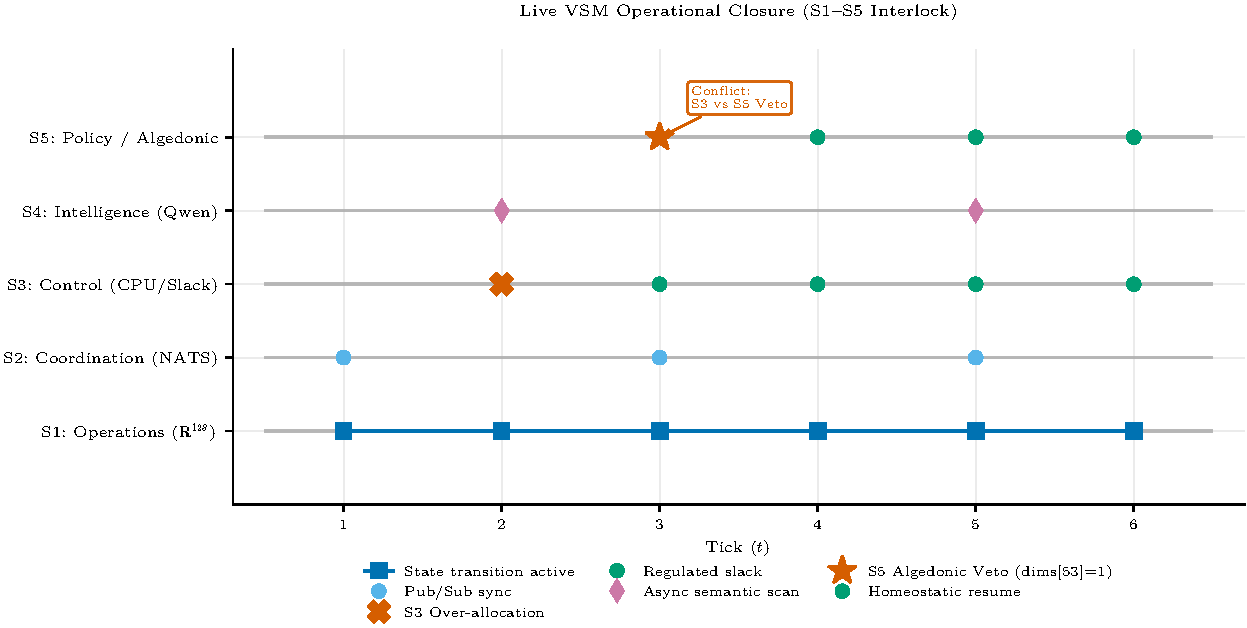
\includegraphics[width=0.88\textwidth]{figures/fig_vsm_operational_closure.pdf}
\caption{Live VSM operational closure timeline across 5 active subsystems (S1--S5) over six ticks, highlighting the precise interlock where S3 over-allocation is intercepted and overridden by the S5 algedonic constitutional veto ($\text{dims}[53]=1$).}
\label{fig:vsm_operational_closure}
\end{figure}

The fixed dip floor ($0.942$) is an exclusive signature of the complete
architecture -- an algedonic signal of S5 in action, not a substrate artefact.
The stability intervention threshold ($\theta_\text{PSI}$) has been
revised from a failure indicator to a precautionary support level,
following the empirical finding that non-viability appears to be
structurally unreachable under normal perturbation.

What remains open is at least as interesting as what has been confirmed.
The thermal response curve has been characterized (EXP-TL-01): degradation
depends on $T \times t$, not temperature alone.
With an adaptive entropy ceiling (EXP-SEN-01) the senescence term is now
measurable and found bounded within a regime; \emph{monotone} senescence
remains undemonstrated and would require external open-system coupling.
The full Lyapunov spectrum has been measured on the reduced 4-state
relaxation subspace (\S\ref{sec:ly01}); the full 128-dimensional Jacobian
remains future work.
The basin floor under impulsive entropic perturbation is now empirically
bounded at $\cos_\text{floor} \approx 0.875$ across six $\delta$ values
(EXP-AB-01), a resilience margin of $0.175$ above the viable threshold;
sustained univariate perturbations have been tested (\S\ref{sec:sustained_noise});
multi-variable sustained perturbation families remain to be tested.

This is a system that can maintain its identity while adapting to
environmental change -- Beer's definition of a viable system.
Whether the geometry of that identity is as rich and robust as the
current experiments suggest, or whether the open questions will reveal
qualitative failures, is the work ahead.


% ??????????????????????????????????????????????????????????????????????????????
\section{Future Work and Broader Programme}
\label{sec:future}

This work documents a single viable system kernel in isolation.
The implications extend across multiple research directions, pursued
in parallel but separate from the core paper.

\subsection*{Measurement and control}

The full Lyapunov spectrum on the 128-dimensional Jacobian of $f_0$
(work item \S\ref{sec:openq} Q4) requires Benettin's method on the full
state space. The partial measurement on the 4-state relaxation subspace
(\S\ref{sec:ly01}) yields a point sink (Kaplan--Yorke dimension $0$);
the full spectrum will replace the $D_\text{eff}$ heuristic with the
formal Kaplan--Yorke dimension on the complete attractor.
Similarly, richer geometric metrics (Hausdorff distance, Wasserstein metric)
may provide finer characterization than cosine similarity.

\subsection*{Environmental interaction}

Beer's original definition of viability requires the system to adapt
to environmental change. The closed-loop experiments reported here
are the foundation; coupling \nucleus{} to a stochastic environment
model (e.g., arrival processes, resource contention) will test
whether adaptation is observable and whether the geometric signature
remains stable under truly novel demands.

\subsection*{Architectural extension: vOS}

The immediate engineering extension is to scale \nucleus{} into a
minimal operating system (vOS). The S4 cognitive layer is already
implemented in Rust with Ollama/Qwen integration (\S\ref{sec:s4}).
The roadmap includes support for multi-kernel coordination (Proxmox
virtualisation), persistent state storage (PostgreSQL), and asset
graphs (Neo4j) to support the full VSF stack in a production setting.
Proxmox integration and the Qwen S4 layer are achieved; PostgreSQL,
Neo4j, and bare-metal vOS deployment remain future work.

\subsection*{Governance and ethics (A0 covenant)}

The ethical axioms A0/A0.1 are currently embedded at compile time as
fixed components of the governance mask --- the ethical faces of $\Omega$
carried in \texttt{dims[53--54]}; the kernel reads those dimensions but has
no runtime mechanism to write them from an external classifier.
A validated sandbox architecture (\textsc{exp-a01-01}) closes this gap
with two distinct layers.
The \emph{enforcement layer} (S5) is a heuristic watchdog that scans the
upward telemetry $\phi^\uparrow$ deterministically and writes
\texttt{dims[53/54]} atomically to a \texttt{tmpfs} signal file that the
kernel reads at each tick; it achieves TPR\,0.93 on A0 violations and
TPR\,0.87 on A0.1 coercion patterns (\textsc{exp-a01-01}, 50-stream
sandbox corpus).
Sandbox experiments confirm the collapse/recovery dynamics: setting
\texttt{dims[53]=1} drives $V\to 0$ within one tick (consistent with
\textsc{exp-g-01}), and resetting the signal restores $V$ to the
attractor baseline $0.102$ within the same tick --- no hysteresis is
observed (Figure~\ref{fig:a0_ethics_performance}).
The \emph{intelligence layer} (S4) runs a Qwen semantic scanner
asynchronously and non-blocking relative to the enforcement write:
when the watchdog fires, S4 provides a post-hoc semantic explanation
for human review; when the watchdog classifies an event window as clean,
S4 scans for novel violation patterns not yet encoded in the heuristic
rules, emitting candidate-rule proposals for operator review (double-loop,
requiring human approval per axiom A5/D4).
A canary integrity probe (injected every ten classifier cycles on known
violations) monitors S4 coherence; failure triggers an algedonic alert
without auto-collapsing $V$, preserving the D4 gate.
This architecture reflects the categorical constraint of
Proposition~\ref{prop:s5_deterministic}: a probabilistic classifier cannot
fulfil the deterministic enforcement contract of S5 (non-negotiable policy
application), but correctly fulfils the S4 contract (environmental scanning,
semantic interpretation, best-effort pattern discovery).
Production deployment of the enforcement wire remains gated on human
approval per axiom A5.
A separate programme explores the mathematics of axiomatic governance
in multi-agent settings --- how axioms remain unviolable under
adversarial perturbation and how they extend to agent coalitions ---
and is documented in a forthcoming manuscript.

\subsection*{Connection to open system thermodynamics}

The fixed perturbation mode (§\ref{sec:governance}, the dip floor at 0.942)
bears structural resemblance to the jump operators of Lindblad's theory
of open quantum systems.
Whether this analogy extends to a quantitative formalism -- e.g.,
interpreting the thermal phase transition as an environmental channel --
is an open question.
Preliminary exploration suggests the connection is more than analogy;
formal development is deferred to a dedicated paper on classical-quantum
analogues in cybernetic systems.

\subsection*{The three-mode programme}

This paper measures Mode 1 (Sec.~\ref{sec:three_modes}). Two directions follow,
stated as objectives rather than results. \textbf{Mode 2 (semantic substrate):}
whether a language model governed by explicit axioms stays within its
constraints more than an ungoverned one is a behavioural, falsifiable question ---
the analogue of the negative controls here --- and is the subject of a companion
paper on symbolic substrates (the inter-layer protocol of Sec.~\ref{sec:vsl}
provides its empirical anchor). \textbf{Mode 3 (cybernetic agent):} the agent
that wraps a language model in review loops, databases, and a formal protocol is
the most literal VSM of the three, and extends toward a viable operating system
with the language model as S4. Both modes share one open objective: to make the
coordinate-free functional $V$ (Sec.~\ref{sec:capstone}) \emph{measurable} on a
reasoning trajectory, not merely definable --- which would require, in Mode 2--3,
the integrity loop (Sec.~\ref{sec:certifier}) to supply the trust that direct
measurement supplies in Mode 1.

\bigskip
\noindent\textbf{Funding.}
This is independent research, conducted without external funding.

\smallskip
\noindent\textbf{Data availability.}
The figure data (Lyapunov spectrum, basin Monte-Carlo, sustained-noise margin,
persistence diagrams) are released as CSV alongside the source. The kernel's
upward telemetry is Merkle-chained and therefore tamper-evident: the released
event logs can be verified against their chain head, a reproducibility property
beyond mere availability.

\smallskip
\noindent\textbf{Code availability.}
The kernel implementation (\nucleus{}) and all experimental tools are
available upon request from the corresponding author (\texttt{luis@tallerpineda.cl}).


% ??????????????????????????????????????????????????????????????????????????????
\section*{Acknowledgements}

The author thanks Marta Cinto, Ricardo Alfaro, Alejandra Rosales, and Marco Trigo
for making space to hear this work.
Professor Ra\'{u}l Fierro (Universidad de Valpara\'{i}so) generously reviewed
an earlier draft; his objection to the original existence argument --- a naive
appeal to Brouwer's theorem on a non-convex region --- directly produced the
convex-core treatment of Theorem~\ref{thm:hybrid_invariance}
(Sec.~\ref{sec:feasible}).
Mathematical formalisation and experiment design were developed in dialogue with
Claude (Anthropic), used here as a research assistant.


% ??????????????????????????????????????????????????????????????????????????????
\bibliographystyle{plainnat}
\bibliography{references}


% ??????????????????????????????????????????????????????????????????????????????
\appendix

\section{Implementation Notes}
\label{app:impl}

\subsection{Kernel architecture}

\nucleus{} is implemented in Rust (stable, 2024 edition).
Relevant modules:
\begin{itemize}
  \item \texttt{src/state\_vector.rs} -- $\sv \in \R^{128}$, blocks A--G;
        \texttt{viable()}, \texttt{lyapunov()},
        \texttt{cosine\_similarity()}.
  \item \texttt{src/vmem.rs} -- vector memory $V_\text{mem}$,
        \texttt{insert()}, \texttt{query\_nearest()}, \texttt{merge\_similar()}.
  \item \texttt{src/attractor.rs} -- \texttt{LyapunovTracker},
        \texttt{StasisVec}, convergence detection.
  \item \texttt{src/s4.rs} -- S4 cognitive client (Ollama/Qwen),
        covenant embedding, $\phi^\downarrow$ channel.
  \item \texttt{src/main.rs} -- experiment dispatch, telemetry.
\end{itemize}

\subsection{Covenant embedding}

The governance covenant is embedded in the binary at compile time
via \texttt{include\_str!()} and verified by SHA-256 before every
S4 call.
This makes the ethical axioms A0/A0.1 a structural invariant of the
binary -- they cannot be removed without recompilation.

\subsection{Persistent worker synchronisation}

\begin{minipage}{\linewidth}
The shutdown-safe Barrier pattern used in \texttt{thermal\_stress\_v3}:
\begin{lstlisting}[language=C, basicstyle=\small\ttfamily,
  frame=single, xleftmargin=1em, breaklines=true, breakatwhitespace=false]
loop {
    start_barrier.wait();
    let stop = stop_flag.load(Relaxed);
    if !stop {
        let n = quota.load(Relaxed);
        let mut acc = 0.0f64;
        for _ in 0..n { acc += sv.cosine_similarity(&st); }
        black_box(acc);
    }
    done_barrier.wait();    // unconditional -- prevents coordinator deadlock
    if stop { break; }
}
\end{lstlisting}
\end{minipage}

\subsection{Experiment specifications}

All experiments are formally specified in
\texttt{docs\slash{}experiments\slash{}<name>\slash{}spec.vsm}
and results are recorded in \texttt{results.vsm} in the same directory.
The master results index is at
\texttt{docs\slash{}experiments\slash{}results\_index.vsm.md}.

\subsection{Reproducibility and logical sequencing}

Each experiment is specified using a formal gate-based notation:
logical conditions (IF condition THEN action) rather than temporal
estimates (X will take Y minutes).
All event timestamps are recorded in ISO 8601 UTC format
(\texttt{started\_at}, \texttt{completed\_at}, \texttt{checked\_at}).
This enables:
\begin{itemize}
  \item Audit trails (who did what when)
  \item Causal ordering (event A caused B iff A.completed\_at $<$ B.started\_at)
  \item Reproducibility checks (actual durations vs baselines)
\end{itemize}
No durations are estimated; observed durations are compared against
historical runs to detect anomalies or improvements.
This methodology avoids false confidence from invented timelines and
provides a clear trigger path for future experiments:
\texttt{IF all gates pass THEN proceed to next phase}.


% ??????????????????????????????????????????????????????????????????????????????
\section{Glossary}
\label{sec:glossary}

This paper crosses cybernetics, dynamical systems, topology, thermodynamics, and
computer science. The glossary is grouped by domain so each community can read
it; the final table maps every measured quantity to the source artefact that
computes it --- certify-not-declare made lexical, so that each claim is traceable
to auditable code.

\paragraph{Cybernetics (Beer, Ashby).}
\begin{description}\itemsep2pt
  \item[VSM] Viable System Model: the recursive S1--S5 organisation of any
    viable system~\cite{beer1972brain}.
  \item[S1--S5] operations, coordination, control, intelligence, policy; S3*
    is the sporadic audit channel.
  \item[Algedonic] a priority alert channel bypassing the normal hierarchy.
  \item[Requisite variety] Ashby's law: a regulator must match the variety of
    what it regulates~\cite{ashby1956introduction}.
  \item[Recursion] each S1 unit may itself be a complete VSM.
\end{description}

\paragraph{Dynamical systems.}
\begin{description}\itemsep2pt
  \item[Attractor] the set a trajectory converges to; here a point sink.
  \item[Lyapunov exponent $\lambda$] mean exponential rate of separation of
    nearby trajectories; $\lambda<0$ is contraction (Benettin's method).
  \item[Lyapunov function $L$] a scalar that decreases along trajectories,
    certifying convergence (distinct from the exponent).
  \item[Basin] the set of initial conditions converging to a given attractor.
  \item[Kaplan--Yorke dimension] a fractal dimension from the spectrum; $0$ for
    a point sink~\cite{kaplan1979chaotic}.
\end{description}

\paragraph{Topology.}
\begin{description}\itemsep2pt
  \item[Betti numbers $\beta_0,\beta_1$] counts of connected components and of
    independent loops; $\beta_0=1\wedge\beta_1=0$ is the point-sink signature.
  \item[Persistent homology] tracks topological features across a scale
    parameter $\varepsilon$; long-lived features are significant.
  \item[Vietoris--Rips complex] the simplicial complex built by connecting
    points within distance $\varepsilon$.
\end{description}

\paragraph{Thermodynamics.}
\begin{description}\itemsep2pt
  \item[Entropy $H$] Shannon entropy of the occupation distribution; $H_\text{max}$
    its ceiling, $H_\text{rest}$ the stasis level.
  \item[Landauer limit] the minimum energy $k_BT\ln 2$ to erase one
    bit~\cite{landauer1961irreversibility}; the outer bound on governance.
  \item[Maxwell's demon] an observer that reduces entropy by measurement;
    here the S4 layer~\cite{maxwell1871theory}.
\end{description}

\paragraph{VSF-specific.}
\begin{description}\itemsep2pt
  \item[$\Omega$] the feasible region $\bigcap_i\{A_i \text{ satisfied}\}$;
    $\Omega_A$ its convex contractive core.
  \item[stasis\_cos] cosine similarity to the stored attractor reference;
    $\theta_\text{viable}=0.70$ is the viability threshold.
  \item[$D_\text{eff}$] active-dimension heuristic (\emph{not} the KY dimension).
  \item[$\varphi^\uparrow/\varphi^\downarrow$] upward telemetry / downward
    command channels between recursion levels.
  \item[Covenant] the S5 policy document; its hash is verified fail-closed at
    boot (axioms A0/A0.1).
  \item[VSL] Viable System Language, the compact protocol notation
    (Sec.~\ref{sec:vsl}).
  \item[$V$] the coordinate-free viability functional
    $\min(g,c,t,m)$ (Sec.~\ref{sec:capstone}).
\end{description}

\paragraph{Artefact register.} Each measured quantity is computed by a named
source artefact:

\begin{table}[!htb]
\centering
\small
\begin{tabular}{lll}
\toprule
Quantity & Symbol & Source artefact \\
\midrule
stasis cosine          & stasis\_cos          & \texttt{state\_vector.rs} \\
Lyapunov spectrum      & $\lambda_i, \hat\sigma_\lambda$ & \texttt{--experiment lyapunov\_spectrum} \\
feasible region        & $\Omega$             & \texttt{omega\_validator.rs} \\
Betti numbers          & $\beta_0,\beta_1$    & \texttt{vr\_complex.rs} ($\mathbb{Z}_2$ homology) \\
basin volume           & --                   & \texttt{--experiment basin\_mc} \\
sustained-noise margin & $m(\sigma)$          & \texttt{--experiment sustained\_noise} \\
calibrated constants   & $\theta,\varepsilon_\text{frontier}$ & \texttt{calibration.rs} \\
\bottomrule
\end{tabular}
\caption{Measured quantities and the source artefacts that compute them.}
\label{tab:artefacts}
\end{table}

\end{document}
